

\documentclass{article}

% Language setting
% Replace `english' with e.g. `spanish' to change the document language
\usepackage[english]{babel}

% Set page size and margins
% Replace `letterpaper' with `a4paper' for UK/EU standard size
\usepackage[a4paper,top=2cm,bottom=2cm,left=3cm,right=3cm,marginparwidth=1.75cm]{geometry}

% Useful packages
\usepackage{amsmath}
\usepackage{amsfonts}
\usepackage{amssymb}   % \checkmark for the coverage table
\usepackage{longtable} % multi-page species coverage table
\usepackage{graphicx}
\usepackage{mathtools}
\usepackage{booktabs}
\usepackage{caption}
\usepackage{subcaption}
\usepackage{braket}

\usepackage{algorithm}
\usepackage{algpseudocode}

\usepackage{tikz}
\usepackage{pgfplots}
\pgfplotsset{compat=1.18}

\usepackage{booktabs}
\usepackage{array}
\usepackage{xcolor}

\usepackage{pdfpages}

\usetikzlibrary{positioning, fit, backgrounds, arrows.meta, calc}

\usepackage[superscript]{cite}

\usepackage[colorlinks=true, allcolors=blue]{hyperref}

% For indentation
\usepackage{parskip} %http://ctan.org/pkg/parskip

% For comments
\usepackage{comment}
\newcommand{\horrule}[1]{\rule{\linewidth}{#1}}
\author{Bob Schreiner}

\begin{document}
\begin{titlepage}
  \centering
  %\vspace*{1cm}
  
\includegraphics[width=0.8\textwidth,height=0.15\textheight,keepaspectratio]{eth-logo-pos.png}

  \horrule{0.5pt} \\[0.4cm] % Thin top horizontal rule
  
\includegraphics[width=0.8\textwidth,height=0.15\textheight,keepaspectratio]{HY__LD02_LogoFV_EN_B3____BW.png}

  \horrule{0.5pt} \\[0.4cm] % Thin top horizontal rule
  \Huge Electronic structure with atomic orbitals on general-purpose
  graphics processing units \\
  \horrule{2pt} \\[0.5cm] % Thick bottom horizontal rule

  \Large{Master thesis in Computational Science and Engineering
  \\ \textit{submitted by}}
  \vspace*{1\baselineskip}

  \LARGE \textbf{Bob Schreiner} \\
  Student number: 20-944-450
  \vspace*{1\baselineskip}

  \Large{\textit{supervised by:} \\ Prof. Dr. Markus Reiher \\}
  \Large{\textit{scientific advisor:} \\ Dr. Susi Lehtola \\}
  \vspace*{2\baselineskip}
  \today

\end{titlepage}
\newpage

\begin{abstract}

  The shift of the computational landscape
  toward general-purpose graphics processing
  units (GPGPUs) for scientific computations, has reopened the
  discussion over established approaches across disciplines. In this
  thesis we provide
  the foundation for a reusable library, capable of harnessing the
  computational power of GPGPUs to perform electronic structure
  calculations in atomic orbital basis sets. The NuKEXC library builds on
  top of the Kokkos ecosystem, which consists of
  performance-portable C++ libraries. NuKEXC
  assembles Fock and Kohn--Sham matrices for any atomic
  orbital basis, including Gaussian-type, Slater-type and numerical atomic
  orbitals. The two-electron terms are approximated via density fitting
  and evaluated by quadrature on grids built with Becke's fuzzy
  Voronoi partitioning
  scheme. We evaluate exchange-correlation terms of the local density
  approximation (LDA) and the generalized gradient approximation
  (GGA) with the same quadrature grids. We show that our quadrature
  schemes deliver total energies
  converged to the \(\mu E_\mathrm{h}\) level, and we benchmark the library on
  the W4-11 test set using Slater-type orbitals. The mean absolute
  deviation of the B3LYP atomization energies improves systematically
  with basis size and settles at the intrinsic accuracy of the
  functional. We also lay out a roadmap towards larger systems and
  the integration of meta-GGA functionals.

\end{abstract}
\tableofcontents

\section{Introduction}\label{sec:intro}
In 1929 John Lennard-Jones formalized the idea to use a linear
combination of atomic orbitals (LCAO) to construct molecular orbitals
(MO).\cite{LennardJones1929}
Twenty years later, Clemens Roothaan used LCAO as a
technique to solve the Hartree--Fock equations computationally for a
general molecule.\cite{Roothaan1951} From this point onward atomic
orbital basis sets have formed the backbone of modern
quantum chemistry programs. The two-electron terms in the
assembly of the Fock matrix posed a major challenge to the early
development of these basis sets. Due to the need
for computational efficiency, the computational chemistry
community almost exclusively used Gaussian-type orbitals (GTOs). The
Gaussian product theorem~\cite{Boys1950} allows for analytic
integration of the two-electron terms and a massive academic effort has been
poured into their efficient evaluation.\cite{King1976, McMurchie1978,Obara1986}

The Hohenberg--Kohn theorems were published in
1964~\cite{Hohenberg1964}, followed shortly by Kohn--Sham density
functional theory (DFT).\cite{Kohn1965} The assembly of the Kohn--Sham
matrix requires the integration of a non-linear functional based on
the electron density. Given the
complexity of the integrand the computational chemistry community was
again in need of computationally efficient schemes that would
allow for the further development of functionals and their
integration. In 1988 Axel Becke proposed
his scheme of fuzzy Voronoi partitioning~\cite{Becke_1988} of the
integration domain.
The partitioning yielded computationally tractable quadrature
schemes that overcame the limitations of earlier approaches to
quantum mechanical calculations.

Curiously, Becke's scheme not only allowed for the efficient
integration of exchange-correlation functionals, but in combination
with a technique called density-fitting it also
delivered a new method, based on quadratures, to evaluate the
two-electron terms in the Fock assembly.\cite{Cohen2002, Watson2003}
While programs that did not use GTOs as their underlying basis set,
such as the Amsterdam density functional (ADF)~\cite{VanLenthe2003,
Franchini2013} program, adapted Becke's
partitioning scheme to
evaluate the two-electron terms, the vast majority of programs used
far more efficient recurrence relations to evaluate those integrals
with GTOs.\cite{Ahlrichs2006}

In recent years the computational landscape has started to
change. Scientific computation has shifted away from personal
computers towards high-performance computing
clusters.\cite{Gavini2023} With the
recent rise of general-purpose graphics processing units (GPGPU) and
the advent of the exascale computing era, computational codes that
were once regarded as state-of-the-art are dwarfed by programs that can
harness the computational power of
GPGPUs.\cite{GalvezVallejo2023, Stocks_2025, WilliamsYoung2021} In
light of this paradigm
shift, computations that were unthinkable thirty years ago are now
within reach.

Much functionality is duplicated across the computational chemistry
programs in use today, partly for reasons of optimization, but also
because the source code of many industry-grade programs is not freely
available. In 2023 Susi Lehtola published a
paper called \emph{A call to arms: Making the case for more reusable
libraries}~\cite{Lehtola2023c}, in which he argues that open source
reusable libraries are necessary to avoid aging and unmaintainable
code bases. Open source codes help researchers reproduce literature
results, and they allow the community to grow and optimize libraries
collectively.

With this work we lay the foundation of a reusable open source
library for the evaluation of the one- and two-electron integrals
constituting the Fock matrix. We also provide the infrastructure to
compute exchange-correlation integrals based on the local density
approximation (LDA) and the generalized gradient
approximation (GGA) necessary to build Kohn--Sham matrices. Our aim is
to make the library as reusable as possible across different basis
sets and hardware providers. We especially target algorithms that are
efficient on modern GPGPUs, but which can also run on local CPUs with
lower accuracy.

This work is organized as follows. Section~\ref{sec:theory}
includes the necessary theory to understand how Fock and Kohn--Sham
matrices are assembled as well as reviewing atomic orbital basis
sets. Section~\ref{sec:comp_methods} reviews the
computational methods that enable us to turn theory into computation,
notably Becke's fuzzy Voronoi partitioning, quadrature schemes and
density fitting.
Section~\ref{sec:Implementation} provides a detailed explanation of
the most crucial
implementations and GPU kernels provided by this work.
Section~\ref{sec:results} shows the convergence properties of our
implementation
as well as how they perform on the W4-11~\cite{Karton11w411} dataset
in terms of accuracy
and wall time. Section~\ref{sec:conclusion} briefly summarizes this
work's results and contributions. Section~\ref{sec:further_research}
gives an outlook on further research opportunities building on this work.

\section{Theory}\label{sec:theory}

We will assume a non-relativistic framework, in which the Schrödinger
equation governs the dynamics of the system. A system consists of
$N_{\text{nuc}}$ nuclei, each of which has a charge $Z_I$, and
$N_{\text{el}}$ electrons, each of which has charge $-1$.
Furthermore, we apply the Born--Oppenheimer approximation, which lets
us separate the Schrödinger equation into an electronic and a
nuclear part. In the remainder we will focus only on the electronic
Schrödinger equation and assume that the nuclei are point
particles, fixed in space. Their coordinates are given by the set
$\{\mathbf R_1, \cdots ,\mathbf{R}_{N_{\text{nuc}}}\}$. We also
assume all basis functions and molecular orbitals to be real-valued
and omit their complex conjugates.

The electronic Schrödinger equation is then given by
\begin{equation}
  \mathbf{\hat H} \mathbf \Psi(\mathbf r_1, \mathbf r_2, \cdots
  ,\mathbf r_{N_{\text{el}}}) = E\mathbf \Psi(\mathbf r_1,
  \mathbf r_2, \cdots ,\mathbf r_{N_{\text{el}}})
  \label{eq:SE}
\end{equation}

$\mathbf{\hat H}$ denotes the electronic Hamiltonian, $\mathbf
\Psi(\mathbf r_1, \mathbf r_2, \cdots ,\mathbf r_{N_{\text{el}}})$ the
many-electron wave function, $E$ the electronic energy, and the set
$\{\mathbf r_1, \cdots ,\mathbf{r}_{N_{\text{el}}}\}$ the coordinates
of the electrons.

\subsection{Hartree--Fock Theory}\label{subsec:HF}

Following the procedure of Roothaan and Hall \cite{Roothaan1951,
Hall1951} to solve the Hartree--Fock equations, we approximate the
electronic wave function $\Psi$ with the anti-symmetrized product of
one-electron functions $\varphi$, called molecular orbitals (MO)

\begin{equation}
  \Psi(\mathbf r_1, \mathbf r_2,\cdots, \mathbf
  r_{N_{\text{el}}}) =
  \frac{1}{\sqrt{N_{\text{el}}!}}\det[\varphi_1\varphi_2 \cdots
  \varphi_{N_{\text{el}}}]  .
  \label{eq:Wavefunction}
\end{equation}

We further approximate the molecular orbitals of spin $\sigma \in
\{\uparrow , \downarrow  \}$ by a linear combination of atomic orbitals $\chi$
\begin{equation}
  \varphi_i^\sigma(\mathbf r) = \sum_{\mu = 1}^{N_{\text{bf}}}
  C^\sigma_{\mu i}\chi_\mu(\mathbf r),
  \label{eq:AO}
\end{equation}

and obtain a generalized eigenvalue problem for each value of $\sigma$
\begin{equation}
  \mathbf F^\sigma  \mathbf C^\sigma =\mathbf S \mathbf
  C^\sigma \mathbf \epsilon^\sigma,
  \label{eq:GenEig}
\end{equation}
where $\mathbf{F}$ is the Fock matrix, $\mathbf{C}$ holds the MO
coefficients, $\mathbf{S}$ is the overlap matrix and
$\mathbf{\epsilon}$ is a diagonal matrix holding the orbital energies.
Since \( \mathbf F^\sigma \) depends on \( \mathbf C^\sigma \) the
generalized eigenvalue problem is non-linear and does not allow for a
closed form solution. The
standard practice of solving this equation is through updating the
matrix \( \mathbf C^\sigma  \) until
self-consistency is reached. The design of
self-consistent field (SCF) solvers is an ongoing research topic,
which is outside of the scope of this work, since we rely on
available reusable implementations.\cite{Lehtola2025}

The Fock matrix can be decomposed into one and two-electron components
\begin{equation}
  F^\sigma_{\mu\nu} = T_{\mu\nu} + V_{\mu\nu}^{\text{nuc}} +
  J_{\mu\nu} - K^\sigma_{\mu\nu},
  \label{eq:FockComponents}
\end{equation}
where

\begin{equation}
  T_{\mu\nu} = -\frac{1}{2} \bra{\mu} \nabla^2 \ket{\nu} =
  \frac{1}{2}\int \nabla\chi_\mu(\mathbf r) \cdot
  \nabla\chi_\nu (\mathbf r) \mathrm d ^3\mathbf r
  \label{eq:kinetic}
\end{equation}

\begin{equation}
  V^{\text{nuc}}_{\mu\nu}
  = -\left \langle \mu \middle |
  \sum_{I=1}^{N_{\text{nuc}}} \frac{Z_I}{|\mathbf{r}-\mathbf
  R_I|} \middle | \nu \right \rangle
  =\sum_{I=1}^{N_{\text{nuc}}}  -Z_I\int
  \frac{\chi_\mu(\mathbf r) \chi_\nu (\mathbf r)}{|\mathbf r -
  \mathbf R_I|} \mathrm d ^3\mathbf r
  \label{eq:nuc}
\end{equation}
are the one-electron contributions and

\begin{equation}
  J_{\mu\nu} =
  \sum_{\lambda\tau}D^\text{tot}_{\lambda\tau}(\mu \nu |
  \lambda \tau) =\sum_{\lambda\tau}D^\text{tot}_{\lambda\tau}
  \iint \frac{\chi_\mu(\mathbf r) \chi_\nu (\mathbf r)
  \chi_\lambda(\mathbf r') \chi_\tau   (\mathbf r')}{|\mathbf r
  - \mathbf{r}'| }  \mathrm d ^3\mathbf r'  \mathrm d ^3\mathbf r
  \label{eq:coulomb}
\end{equation}

\begin{equation}
  K^\sigma_{\mu\nu} =
  \sum_{\lambda\tau}D^\sigma_{\lambda\tau}(\mu \lambda | \nu
  \tau   ) =\sum_{\lambda\tau   }D^\sigma_{\lambda\tau   }
  \iint \frac{\chi_\mu(\mathbf r) \chi_\lambda (\mathbf r)
  \chi_\nu(\mathbf r') \chi_\tau   (\mathbf r')}{|\mathbf r -
  \mathbf{r}'| } \mathrm d^3\mathbf r' \mathrm d^3\mathbf r
  \label{eq:exchange}
\end{equation}

are the two-electron contributions. $D^\sigma_{\lambda\tau}$ is the
density matrix and is defined as

\begin{equation}
  D^\sigma_{\lambda\tau} =
  \sum_{i=1}^{N_\text{occ}}f_iC^\sigma_{\lambda
  i}C^\sigma_{\tau i},
  \label{eq:density_matrix}
\end{equation}
where $f_i$ is the occupation number, with $0 \leq f_i \leq 1$, and
$D^\text{tot}_{\lambda\tau} = D^\uparrow_{\lambda\tau} +
D^\downarrow_{\lambda\tau}$.

\begin{equation}
  S_{\mu\nu} =  \braket{\mu | \nu} = \int \chi_\mu(\mathbf r)
  \chi_\nu (\mathbf r) \mathrm d ^3 \mathbf r
  \label{eq:overlap}
\end{equation}
is the overlap between the basis functions $\chi_\mu$ and $\chi_\nu$.

\subsection{Density Functional Theory}\label{subsec:DFT}

Within Kohn--Sham DFT, the two-electron exchange term of
\eqref{eq:exchange} is replaced by an exchange-correlation (xc)
energy functional $E_{xc}[\rho^\sigma]$, evaluated on the density
$\rho^\sigma(\mathbf r)$ defined by

\begin{equation}
  \rho^\sigma(\mathbf r) =
  \sum_{\mu\nu}D^\sigma_{\mu\nu}\chi_\mu(\mathbf r) \chi_\nu(\mathbf r).
  \label{eq:density}
\end{equation}

Unlike the Coulomb and exact exchange integrals, $E_{xc}[\rho]$ is in
general a nonlinear functional of the density and therefore admits no
analogous two-electron integral representation.

The contribution of the xc term to the Kohn--Sham Fock matrix is
\begin{equation}
  V^{xc}_{\mu\nu} = \int \chi_\mu(\mathbf r)\, v_{xc}(\mathbf
  r)\, \chi_\nu(\mathbf r)\, \mathrm d^3 \mathbf r,
  \label{eq:xc-matrix}
\end{equation}
where $v_{xc}(\mathbf r)$ is the xc potential, obtained from the
functional derivative of $E_{xc}$ with respect to the density,
\begin{equation}
  v_{xc}(\mathbf r) = \frac{\delta E_{xc}[\rho^\sigma]}{\delta
  \rho^\sigma(\mathbf r)}.
  \label{eq:xc-potential}
\end{equation}

For hybrid functionals, $E_{xc}$ additionally contains a fraction
$c_x$ of exact Hartree--Fock exchange,
\begin{equation}
  E_{xc}^{\text{hyb}} = c_x E_x^{\text{HF}} + (1-c_x) E_x^{\text{DFT}}
  + E_c^{\text{DFT}},
  \label{eq:hybrid-xc}
\end{equation}
where $E_x^{\text{HF}}$ is built from $K^\sigma_{\mu\nu}$.

Collecting these contributions, the Kohn--Sham matrix assembled during
each SCF cycle reads
\begin{equation}
  F^\sigma_{\mu\nu} = T_{\mu\nu} + V^{\text{nuc}}_{\mu\nu} + J_{\mu\nu}
  + V^{xc}_{\mu\nu} - c_x K^\sigma_{\mu\nu},
  \label{eq:ks-matrix}
\end{equation}
which reduces to the Hartree--Fock matrix \eqref{eq:FockComponents} for
$c_x = 1$ and $V^{xc}_{\mu\nu} = 0$, and to a pure Kohn--Sham matrix for
$c_x = 0$.

\subsection{Basis Sets}\label{subsec:basis_sets}

Basis sets are almost as old as the field of quantum chemistry
itself. In equation \eqref{eq:AO}, we stated that molecular orbitals
are approximated by a linear combination of atomic orbitals, but we
never specified the exact nature of those atomic orbitals. This is
because the expansion is not unique, in contrary there exists  a
whole zoo of atomic orbital basis set expansions. In each
of the following subsections we will give an overview of one family
of atomic basis set expansions.

\subsubsection{Slater-Type Orbitals}\label{subsubsec:sto}
Normalized Slater-type orbitals (STOs) can be defined as
\begin{equation}
  \mathcal S_\mu (\mathbf r ) = \mathcal S(\zeta,
  n,l,m;r,\theta,\phi) =
  \frac{(2\zeta)^{n+\frac{1}{2}}}{[(2n)!]^\frac{1}{2}} r^{n-1}
  e^{-\zeta r}Y_{lm}(\theta,\phi),
\end{equation}
where $\zeta$ is a positive real number, $n$ is their principal quantum
number, $l$ is their angular momentum and $m$ is their magnetic
quantum number. The restrictions on the quantum numbers are
$n>l\geq0$ and $-l\leq m \leq l$. $Y_{lm}(\theta,\phi)$ are the real
spherical harmonics defined as
\begin{equation}
  Y_{lm}(\theta,\phi) =
  \left(\frac{(2l+1)(l-|m|)!}{2\pi(l+|m|)!}\right)^{1/2} \times
  \begin{cases}
    \cos(|m|\phi) P_l^{|m|}(\cos\theta) & l \geq m > 0 \\[2mm]
    \dfrac{1}{\sqrt{2}} P_l^0(\cos\theta) & m = 0 \\[2mm]
    \sin(|m|\phi) P_l^{|m|}(\cos\theta) & -l \leq m < 0.
  \end{cases}
  \label{eq:spherical_harm}
\end{equation}

$P^m_l$ are the associated Legendre
functions.\cite{Cohen2002,Chong2004, Chong2005}

STOs are arguably the most straightforward guess for a basis set
when doing molecular calculations in the LCAO framework, because STOs
are modeled after the analytical solutions to the hydrogen
atom.\cite{Slater1930} It is only when being faced with the
challenges of computing the two-electron integrals \eqref{eq:coulomb}
and \eqref{eq:exchange}, that STOs prove problematic. Since
the numerical evaluation of the two-electron integrals is
computationally very expensive for
STOs,~\cite{Weniger2009, FernandezRico1998} researchers have
focused their attention on other basis sets that are not plagued by
the same inefficiencies, namely Gaussian-type
orbitals (GTOs).\cite{Hill2012, Boys1950}

\subsubsection{Gaussian-Type Orbitals}\label{subsubsec:gto}
Normalized GTOs can be defined as
\begin{equation}
  \mathcal G_\mu(\mathbf r ) = \mathcal G(\alpha, l,m;r,\theta,\phi)
  = \sqrt{\frac{2^{l+2} (2\alpha)^{l+\frac{3}{2}}}{(2l+1)!! \sqrt{\pi}}}
  r^{l} e^{-\alpha r^2}Y_{lm}(\theta,\phi),
\end{equation}

where $\alpha$ is a positive real number, $l$ is their angular momentum and
$m$ is their magnetic quantum number. The restrictions on the quantum
numbers are $l \geq 0$ and $-l\leq m \leq l$. $Y_{lm}(\theta,\phi)$
are the real spherical harmonics defined in equation
\eqref{eq:spherical_harm}.\cite{Hill2012}

GTOs are the most popular atom-centered basis set expansion in the
quantum chemistry community,\cite{Hill2012} mainly
because of the Gaussian product theorem.\cite{Boys1950} The theorem
states that the product of two Gaussian functions is
also a Gaussian function, and therefore allows for the analytical
integration of the two-electron integrals defined in equations
\eqref{eq:coulomb} and
\eqref{eq:exchange}. The Gaussian product theorem, combined with
efficient recursive evaluation strategies, such as the Obara--Saika
scheme, has made the evaluation of the two-electron integrals
\eqref{eq:coulomb} and \eqref{eq:exchange} tractable and
efficient.\cite{Obara1986, Ahlrichs2006}

GTOs come with their own set of drawbacks though. GTOs lack certain
properties that one would expect the ``true'' underlying basis set
should fulfill. For example, one would expect the basis functions to
exhibit a cusp at the nucleus; this condition is known as the
Kato-cusp condition.\cite{Kato1957} The radial decay of Gaussian
functions, which is much faster than that of STOs, is another typical
drawback, which makes long-range interactions harder to capture in
molecular calculations.\cite{Hill2012}

The drawbacks of GTOs have not gone unnoticed and the literature is
rich in basis sets that have been developed to lessen the side
effects of GTOs. The usual compromise that is made when using a GTO
basis set is to add more GTOs to the original basis set,
usually doubling or even tripling the original number of basis
functions.\cite{Ditchfield1971, Dunning1989} The speedup gained from
using analytical integration over numerical quadrature has outweighed
the need for more basis functions in the past.

\subsubsection{Numerical Atom-Centered Orbitals}\label{subsubsec:nao}
Numerical atom-centered orbitals (NAOs) can be defined as
\begin{equation}
  \mathcal N_\mu(\mathbf r)= \mathcal N (n,l,m;r,\theta,\phi) =
  \frac{u_{nl}(r)}{r}Y_{lm}(\theta,\phi),
\end{equation}
where $n$ is their principal quantum number, $l$ is their angular
momentum and $m$ is their magnetic quantum number. The restrictions on
the quantum numbers are $n>l\geq0$ and $-l\leq m \leq l$.
$Y_{lm}(\theta,\phi)$ are the real spherical harmonics
defined in equation \eqref{eq:spherical_harm}.\cite{Lehtola2019}

NAOs can be considered a generalization of STOs and GTOs, since we
could replace their radial part by analytical expressions and recover
a particular basis that way.\cite{Lehtola2019b} Using an analytical
expression for $B(r)$ would defy the purpose of using NAOs in the
first place though, so NAOs are usually not defined analytically,
but, as the name suggests, are only available numerically. Generating
NAO basis sets is usually done by solving a simplified radial
differential equation
for an individual atom, utilizing numerical methods such as the finite
element method (FEM) and storing the results
numerically.\cite{Blum_2009,Lehtola2019,Lehtola2019a,Lehtola2023b} In
the case of HelFEM $u_{nl}(r)$ consists of a linear
combination of Lagrange Interpolating Polynomials
(LIP)\cite{Lehtola2019, Lehtola2019a} or Hermite Interpolating
Polynomials (HIP)\cite{Lehtola2023b}, which can be tabulated and passed on to an
integral evaluation routine.

\section{Computational Methods} \label{sec:comp_methods}
In this section we will cover the theory of the computational methods
we used to compute the Fock/KS matrices. The actual implementations
are explained in Section~\ref{sec:Implementation}.

\subsection{Quadratures}\label{subsec:quadratures}
Quadrature schemes are a tool to approximate integrals over a domain
$\Omega$. A quadrature scheme is usually represented by a set of
tuples $\{(\mathbf r_q, w_q)\}_{q=1}^{N_{\text{quad}}}$, where
$\mathbf r_q$ are the quadrature points and $w_q$ are the quadrature
weights. The integral can then be approximated by a weighted sum over
function evaluations

\begin{equation}
  I = \int_\Omega F(\mathbf r) \mathrm d^3 \mathbf r \approx
  \sum_{q=1}^{N_{\text{quad}}}F(\mathbf r_q)w_q \quad.
  \label{eq:global_quadrature}
\end{equation}

The generation of quadrature points and quadrature weights can
differ drastically from one scheme to another and there isn't a
one-size-fits-all solution. It is common that a given quadrature
scheme is specifically designed for a family of integrands $F$ or a
domain $\Omega$ or both.

We chose to implement Becke's quadrature scheme in our integral
evaluation library, since it has stood the test of time and is the
standard integral evaluation tool in most molecular quantum chemistry
programs today.\cite{Becke_1988, Franchini2013}

\subsubsection{Becke's Molecular Partitioning Scheme}
Becke's molecular partitioning scheme,\cite{Becke_1988} also known as
fuzzy Voronoi partitioning, is a method in which the integral we want
to compute is split into a weighted sum of sub-integrals. Each
sub-integral is evaluated in polar spherical coordinates,
centered at a nucleus, by means of traditional quadrature schemes.

The goal of this scheme is to find relative weight functions $p_n$,
one for each nucleus, such that for all $\mathbf r$,

\begin{equation}
  \sum_n p_n(\mathbf r) = 1
  \label{eq:partition_weights_unity}
\end{equation}

and such that $p_n(\mathbf r)$ has value unity in the vicinity of its
own nucleus, but vanishes continuously near any other nucleus.

Our globally defined integrand $F$ can then be decomposed into
single-center components $F_n(\mathbf r)$,

\begin{equation}
  F(\mathbf r) = \sum_n F_n(\mathbf r),
  \label{eq:integrand_decomposed}
\end{equation}
where

\begin{equation}
  F_n(\mathbf r) = p_n(\mathbf r) F(\mathbf r).
  \label{eq:partial-integrand_definition}
\end{equation}

The integral $I$ in equation \eqref{eq:global_quadrature} can then be
rewritten as a sum over single-center integrations $I_n$ over each of
the nuclei in the system

\begin{equation}
  I = \sum_n I_n,
  \label{eq:integral_decomposed}
\end{equation}
where

\begin{equation}
  I_n = \int F_n(\mathbf r)\mathrm d^3\mathbf r.
  \label{eq:partial-integral_definition}
\end{equation}

Given a set of $N_\text{nuc}$ spherical quadrature grids, each with
$n_\text{quad}$ points,
$\{\{(\mathbf r_{nq},
w_{nq})\}_{q=1}^{n_{\text{quad}}}\}_{n=1}^{N_{\text{nuc}}}$, where we
denote $(\mathbf r_{nq},w_{nq})$ the $q$-th quadrature element
generated by the $n$-th quadrature grid, we construct the
partitioning weights by computing the confocal elliptic coordinate
$\mu$ defined as

\begin{equation}
  \mu_{ij} = \frac{r_i - r_j}{R_{ij}},
  \label{eq:mu_ij}
\end{equation}

where $r_i$ denotes the scalar distance between the given quadrature
point $\mathbf r_q$ and the $i$-th nucleus and $R_{ij}$ denotes the
distance between nucleus $i$ and nucleus $j$. Then, we apply a
polynomial smoothing function given as

\begin{align}
  h(\mu)   &= \frac{3}{2} \mu - \frac{1}{2} \mu^3
\end{align}
$k$ times, resulting in

\begin{align}
  f_1(\mu) &= h(\mu) \\
  f_k(\mu) &= h(f_{k-1}(\mu)),
\end{align}

where $f_k$ has a smoothly varying value in the interval $[-1,1]$.
The value of $k$ controls the sharpness of the partition, $k=3$ is
the standard choice in most computer programs\cite{Becke_1988,
Franchini2013}. The result is then linearly mapped into the interval $[0,1]$ by

\begin{align}
  s_k(\mu) &= \frac{1}{2} [1-f_k(\mu)].
\end{align}

Finally we construct the normalized molecular partitioning weights $p_n$
\begin{align}
  P_n(\mathbf r) &= \prod_{j \neq n} s_k(\mu_{nj}) \\
  p_n(\mathbf r) &= \frac{P_n(\mathbf r) }{ \sum_m P_m(\mathbf r)}.
  \label{eq:partition_weight_def}
\end{align}

After constructing the partitioning weights $p_n$, each quadrature
weight $w_{nq}$ gets scaled by its corresponding partitioning function

\begin{equation}
  w'_{nq} = p_n(\mathbf r_{nq}) w_{nq},
  \label{eq:rescaled_weights}
\end{equation}

so that our final integral evaluation reads

\begin{equation}
  I \approx
  \sum_{n=1}^{N_\text{nuc}}\sum_{q=1}^{n_\text{quad}}w'_{nq}F(\mathbf
  r_{nq}).
\end{equation}

The construction of the relative weight functions is not unique
though and improvements have been made over Becke's original
proposal.
Laqua et al. introduced a construction that is close to the
original proposal of Becke, but yields more robust results and has
better screening properties.\cite{Laqua2018} In their construction
$\mu_{ij}$ in equation \eqref{eq:mu_ij} is modified to

\begin{align}
  \mu_{ij}^{\text{mod}} &= \frac{r_i -
  r_j}{\min(R_{\text{cutoff}}, R_{ij})}, \\
  \mu_{ij}^{\text{mod,cutoff}} &=
  \begin{cases}
    -1 , & \mu_{ij}^{\text{mod}} \leq -1 \\
    1 , & \mu_{ij}^{\text{mod}} \geq 1\\
    \mu_{ij}^{\text{mod}}, & \text{otherwise}
  \end{cases}
  \label{eq:mu_mod}
\end{align}

and $\mu_{ij}^{\text{mod,cutoff}}$ is used in all subsequent
computations instead of $\mu_{ij}$. $R_{\text{cutoff}} = 5$ bohr
provided optimal results in their tests.

\subsubsection{Quadrature Grids}
Now that we know how to generate the partitioning weights $p_n$ from
a set of quadrature grids $\{\{(\mathbf r_{nq},
w_{nq})\}_{q=1}^{n_{\text{quad}}}\}_{n=1}^{N_{\text{nuc}}}$, we
examine how the quadrature grids are generated.
Assuming that we are given the position of the center $\mathbf r_n$,
in our case this would be the position of a nucleus, we can rewrite
the single center sub-integral \eqref{eq:partial-integral_definition}
in spherical polar coordinates

\begin{equation}
  I_n = \int_{0}^{2\pi} \int_{0}^{\pi} \int_{0}^\infty
  F_n(r,\theta,\phi)r^2 \sin \theta \,\mathrm dr \, \mathrm d\theta
  \,\mathrm d\phi.
  \label{eq:I_polar}
\end{equation}

Alternatively, employing a quadrature formula for direct
two-dimensional integration on the surface of the unit sphere, we can
rewrite the integral as

\begin{equation}
  I_n = \int_{S^2}\int_0^{\infty} F_n(r,\Omega)r^2  \mathrm dr \,
  \mathrm d\Omega,
  \label{eq:I_solid}
\end{equation}
where $\Omega$ denotes solid angle and $S^2$ is the unit sphere.

The standard approach is then to use separate quadrature schemes for
the angular and radial components. The most commonly employed angular
quadrature grids are the ones derived by Lebedev, since they
integrate the spherical harmonics exactly up to a given order $l$,
just as the Gauss--Legendre quadrature integrates
polynomials up to a given order $n$ exactly.\cite{Lebedev1976, Lebedev1977}

The case is not so clear-cut for the radial quadrature schemes,
because not only do we have to choose an appropriate quadrature
scheme, but we also need to choose a radial transformation that maps
the original radial quadrature points into the interval $[0,\infty)$.
In the following we will have a look at the radial quadrature scheme
proposed by Becke in his original work, and the arguably most used
radial quadrature grid proposed by Treutler and Ahlrichs.
\cite{Becke_1988, Treutler1995}

Becke proposed to use the Gauss--Chebyshev quadrature points in the
interval $x\in [-1,1]$ and use the radial transformation

\begin{equation}
  r = \xi_n\frac{1+x}{1-x},
  \label{eq:Becke_radial}
\end{equation}

where $\xi_n$ stands for half of the Bragg--Slater radius of the
respective nucleus, except for hydrogen, where Becke did not apply
the factor $1/2$.

Treutler and Ahlrichs later reviewed Becke's approach to the
construction of the radial grid and found that the concentration of
the quadrature points was not dense enough around $r_n$ and that too
many points were generated far away from the nucleus leading to a
waste of quadrature points. To mitigate those problems they proposed
the radial transformation

\begin{equation}
  (\text{M3}) : r = \frac{\xi}{\ln 2} \ln \frac{a+1}{1-x}
  \label{eq:M3}
\end{equation}

as well as the extended parametrized version

\begin{equation}
  (\text{M4}) : r = \frac{\xi}{\ln 2} (a+x)^\alpha \ln \frac{a+1}{1-x},
  \label{eq:M4}
\end{equation}

where they stated that $\alpha = 0.6$ yielded the best results in
combination with $a = 1$ and the Chebyshev quadrature of the second
kind, $x\in[-1 ,1]$ .

They also published a table for optimized values of $\xi$ for the
case of the (M4) grid, but it should be noted that their
optimizations were conducted using a Gaussian basis set
(Section~\ref{subsubsec:gto}).

Note that the generation of quadrature grids is an
ongoing research topic and that the literature is rich in different
approaches.\cite{Becke_1988, Gill1993, Murray_1993, Goursot1994,
  Johnson1994, Treutler1995, Mura_1996,
  adaptivenumericalintegratorformolecularintegrals1998, Gill2003,
Efficient2004} The stability of the quadrature grids has been
heavily debated in the past and the consensus in the literature is
that quadrature grids need to be well converged, i.e. have enough
quadrature points, in order to yield meaningful results, especially
when computing energy gradients.\cite{Johnson_1993, Baker1994, Papas2006}

\subsection{Density Fitting \& Resolution of the
Identity}\label{subsec:density_fitting}

The one-electron integrals fit the form of
\eqref{eq:global_quadrature} perfectly. For example, if we wish to
compute $T_{\mu\nu}$ from \eqref{eq:kinetic}, we replace $F(\mathbf
r)$ by $\nabla \chi_\mu (\mathbf r) \cdot \nabla \chi_\nu(\mathbf r)$
and provide a set of quadrature grids. The procedure explained in
Section~\ref{subsec:quadratures} then gives us the corresponding approximation.

In order to compute the Fock matrix though, we need to find a procedure
that lets us approximate the two-electron integrals defined in
\eqref{eq:coulomb} and \eqref{eq:exchange} as well. To achieve this
goal we employ density fitting, also known as the resolution
of the identity, to reduce the two-electron integrals to one-electron
integrals of the form \eqref{eq:global_quadrature}. We closely follow
the procedures described by Cohen and Handy \cite{Cohen2002} for the
Coulomb integral and Watson et al.  \cite{Watson2003}  for the
exchange integral.

Density fitting approximates the density $\rho(\mathbf r)$ as a
linear combination of the auxiliary basis $\tilde \chi_\alpha(\mathbf
r)$ to give the fitted density $\tilde \rho(\mathbf r)$, defined as

\begin{equation}
  \tilde \rho(\mathbf r) =
  \sum_{\alpha}d_{\alpha}\tilde\chi_\alpha(\mathbf r).
  \label{eq:fitted_density}
\end{equation}

The procedure of Cohen and Handy relies on minimizing the Coulomb
energy $E_C$ of the difference density $\Delta\rho(\mathbf r)$.

\begin{align}
  \Delta \rho (\mathbf r) &= \rho(\mathbf r) - \tilde\rho(\mathbf r) \\
  E_C[\Delta \rho] &= \iint \frac{\Delta\rho(\mathbf
  r)\Delta\rho(\mathbf r ')}{|\mathbf r - \mathbf r '|} d
  \mathbf r d \mathbf r '
\end{align}

The minimization yields a set of normal equations for $d_\alpha$

\begin{equation}
  \sum_\beta (\alpha|\beta) d_\alpha =  \sum_{\mu \nu}
  (\mu \nu |\beta)D^{\text{tot}}_{\mu \nu}.
\end{equation}

By substituting $d_\alpha$ back into \eqref{eq:fitted_density}, and
substituting the fitted density into equations \eqref{eq:coulomb} and
\eqref{eq:exchange}, we obtain the following approximations for the
Coulomb and exchange integrals

\begin{equation}
  J_{\mu\nu} \approx \tilde J_{\mu\nu} = \sum_{\alpha \beta \lambda\tau}
  (\mu \nu | \alpha)(\alpha |
  \beta)^{-1}(\beta|\lambda\tau)D^{\text{tot}}_{\lambda\tau}
  \label{eq:coulomb-RI}
\end{equation}

\begin{equation}
  K_{\mu\nu}^\sigma \approx \tilde K_{\mu\nu}^\sigma = \sum_{\alpha
  \beta\lambda\tau}
  (\mu \lambda | \alpha)(\alpha |
  \beta)^{-1}(\beta|\nu\tau)D^\sigma_{\lambda\tau}
  \label{eq:exchange-RI}
\end{equation}

The 3-center integrals can then be expanded as follows

\begin{align}
  (\mu\nu|\alpha) =
  \iint \frac{\chi_\mu(\mathbf r) \chi_\nu (\mathbf r)
  \tilde\chi_\alpha(\mathbf r')}{|\mathbf r - \mathbf{r}'| }
  \mathrm d^3\mathbf r' \mathrm d^3\mathbf r
  = \int \chi_\mu(\mathbf{r})\chi_\nu(\mathbf{r})
  \tilde{V}_\alpha(\mathbf{r})
  \mathrm d^3\mathbf{r},
  \label{eq:3-center-ri}
\end{align}

where we defined $\tilde V_\alpha(\mathbf r)$ as

\begin{align}
  \tilde V_\alpha(\mathbf r) =
  \int \frac{\tilde\chi_\alpha(\mathbf r')}{|\mathbf r -
  \mathbf{r}'| } \mathrm d^3\mathbf r',
  \label{eq:potential-chi}
\end{align}
i.e. the potential of $\tilde\chi_\alpha$. Note that $\tilde V_\alpha$ is
known analytically for STOs \cite{Cohen2002}.

Similarly we can rewrite $(\alpha|\beta)$ as

\begin{align}
  (\alpha|\beta) =
  \iint \frac{\tilde\chi_\alpha(\mathbf
  r)\tilde\chi_\beta(\mathbf r')}{|\mathbf r - \mathbf{r}'| }
  \mathrm d ^3\mathbf r' \mathrm d^3\mathbf r = \int
  \tilde\chi_\alpha(\mathbf{r}) \tilde V_\beta(\mathbf{r}) d\mathbf{r}.
  \label{eq:2-center-ri}
\end{align}

How $(\alpha|\beta)$ is inverted is implementation dependent and will
be covered in Section~\ref{sec:Implementation}.

The integrals \eqref{eq:3-center-ri} and \eqref{eq:2-center-ri} can
then be approximated by the quadrature scheme explained in the previous section.

\section{Implementation Details}\label{sec:Implementation}

This section provides a detailed explanation of our implementations
of the computational methods outlined in section
\ref{sec:comp_methods}. Since we aim to build a reusable library, we
have to be careful when choosing the framework, which we want to
build our library upon. First and foremost we should check if a
similar reusable library already exists and can be extended to our needs.

During our literature research we examined the reusable library GauXC
\cite{WilliamsYoung2021, WilliamsYoung2020}. GauXC is indeed a
strong candidate; the library provides a broad set of functionality
to create quadrature grids, evaluate Becke's partitioning scheme and
integrate Gaussian basis sets with excellent scaling on GPGPUs. The
main drawback of GauXC is that its code base is split into
multiple programming languages. The authors chose to write the main library
interface in C++, and the GPU kernels in CUDA and HIP.

While it is standard practice for a low level library to have a
hardware specific implementation, we deem this paradigm to be
unmaintainable for a scientific computing library, whose aim it is
to be reused across different programs. If a change is made to one
kernel on the CUDA side, after having tested and optimized this
kernel, it needs to be rewritten and re-optimized in HIP and
vice versa. While there exist tools like hipify, which promise to
take care of this task, they only work for simple kernels,
where a one to one correspondence between functions exists. For
complex tasks the functionalities that CUDA and HIP provide are
drastically different and the hard truth is that in research codes a
kernel will actually only be implemented in one framework and the
other one will be ignored. We came to the conclusion that in order to build a
maintainable and truly reusable library, we would have to take a
different approach, where the implementations themselves remain
hardware agnostic.

\subsection{Kokkos}\label{subsec:Kokkos}

The Kokkos ecosystem provides a performance portable solution to
write modern C++ in a hardware agnostic way. The ecosystem consists
of three main parts, Kokkos Core \cite{CarterEdwards2014, Trott2022},
Kokkos Kernels, \cite{Rajamanickam2021} and Kokkos Tools
\cite{Hammond2018}. Kokkos Core provides the base functionality to
write parallel algorithms in C++. During the compilation step, Kokkos
can then map an algorithm onto the desired target architectures
according to architecture-specific rules to achieve best performance.
Kokkos Kernels is a highly optimized software library for linear
algebra and graph algorithms. The library provides native Kokkos
kernels as well as the option to use third party implementations.
Kokkos Tools is a software interface consisting of profiling and
debugging tools. The tools are lightweight and are meant to
cause minimal friction with Kokkos applications while providing
valuable insights into the Kokkos kernels.

Although Kokkos sounds like it would solve all of our problems, we
observed clear drawbacks during the design and testing of our
library. For example, the software developer is only able to write the
kernels according to Kokkos' patterns, which means the developer has
less explicit control over the data management and scheduling than
one would have in a language like CUDA or HIP. The Kokkos kernels also
provide a broad range of linear algebra functionality, but they fall
far short of supporting all BLAS and LAPACK routines. As we will
show later, in Section~\ref{subsubsec:dense_la_rij_rik} we needed to adapt an
algorithm that originally made use of a Cholesky decomposition to
instead use a singular value decomposition, because the Cholesky
decomposition subroutine of a general symmetric positive definite
matrix is not implemented in Kokkos Kernels at the time of writing.

Table~\ref{tab:kokkos_hw_mapping} summarizes how the Kokkos
abstractions used throughout this work map onto the underlying GPU
hardware.

\begin{table}[H]
  \centering
  \caption{Correspondence between Kokkos abstractions and GPU
  hardware components.}
  \label{tab:kokkos_hw_mapping}
  \begin{tabular}{@{}l l@{}}
    \toprule
    Kokkos abstraction & Hardware component \\
    \midrule
    \texttt{DefaultHostExecutionSpace}      & Host \\
    \texttt{parallel\_for} / \texttt{parallel\_reduce}
    launch & Thread Processor (grid/work distributor) \\
    Team (\texttt{TeamPolicy} league member) & One
    resident thread block on one SM \\
    \texttt{TeamThreadRange} / \texttt{TeamVectorRange} &
    Stream Processors within an SM \\
    \texttt{team\_scratch} / \texttt{PerTeam} scratch &
    Shared Memory (per SM) \\
    \texttt{team\_barrier()}                & Instruction
    Fetch/Dispatch (block-level sync) \\
    Plain \texttt{View} (global memory)     & L1 / L2
    cache $\to$ FB (device DRAM) \\
    \texttt{MemoryTraits<RandomAccess>} \texttt{View} &
    Texture Fetch unit \\
    \bottomrule
  \end{tabular}
\end{table}

\subsection{Grid Construction}\label{subsec:grid_construction}

We construct the quadrature grid based on the positions of the nuclei
$\{\mathbf R_i\}_{i=1}^{N_\text{nuc}}$. For each nucleus we construct
a spherical quadrature grid with \texttt{IntegratorXX}~\cite{IntegratorXX}, and
then shift these quadrature grids such that they are centered at their specific
parent nucleus. We then flatten the quadrature points and weights into one
dimensional \texttt{Kokkos::View}s of size $N_\text{nuc}\cdot
n_\text{quad}$. Note that the number of quadrature points generated
around one nucleus could be adjusted based on its charge. This would
allow, for example,
heavier nuclei to have more quadrature points surrounding them.
To keep track of which quadrature point was generated around which nucleus we
create a \texttt{Kokkos::View} called
\textit{owner} of size $N_\text{nuc}\cdot
n_\text{quad}$.

Now that we have fixed the positions of the quadrature points, we can move on to
step two of our grid construction and compute the partitioning
weights. To compute Becke's partitioning scheme we make use of
Kokkos' Data Parallelism
paradigm as well as Kokkos' Hierarchical Parallelism paradigm.
The entire control-flow is schematically represented in Figure
\ref{fig:becke_team_flow} and all memory allocations are documented
in Table~\ref{tab:becke_team_memory_allocations}.

First we compute the matrix $R_{ij}$, denoting the distance between
nucleus $i$ and nucleus $j$, and store it in a global
\texttt{Kokkos::View}, accessible by
all threads. Then we create one
\texttt{Kokkos::Team} for each quadrature point in $\{\{(\mathbf r_{nq},
w_{nq})\}_{q=1}^{n_{\text{quad}}}\}_{n=1}^{N_{\text{nuc}}}$. Each
team allocates two arrays of scratch memory in the L1 cache, one for
the distances from the quadrature points to the nuclei $r_i$ and one for
the partitioning weights $P_i$. Each team then executes the following GPU kernel
simultaneously.

Each team launches a
$\texttt{Kokkos::TeamVectorRange}$ parallel region, where each thread
fills one entry in the $r_i$ cache. After the team has finished
filling the scratch, they proceed to calculate $\mu_{ij}$ and
$P_i$ according to Equations~\eqref{eq:mu_ij} and
\eqref{eq:partition_weight_def}, again using a
$\texttt{Kokkos::TeamVectorRange}$ parallel region. Next the
threads compute the normalization constant $Z = \sum_m
P_m(\mathbf{r}_{nq})$ with a parallel reduce over all nuclei
and each team computes the normalized partitioning weight
$p_n(\mathbf{r}_{nq})$. Finally
each team scales its quadrature point's original weight by the normalized
partitioning weight, according to
\eqref{eq:rescaled_weights}.

\begin{figure}[H]
  \centering
  % --- Vertical flowchart: the pipeline reads top to bottom. Height-bounded
  % (not width-bounded) so the column keeps a legible box size. ---
  \resizebox{!}{0.50\textheight}{%
    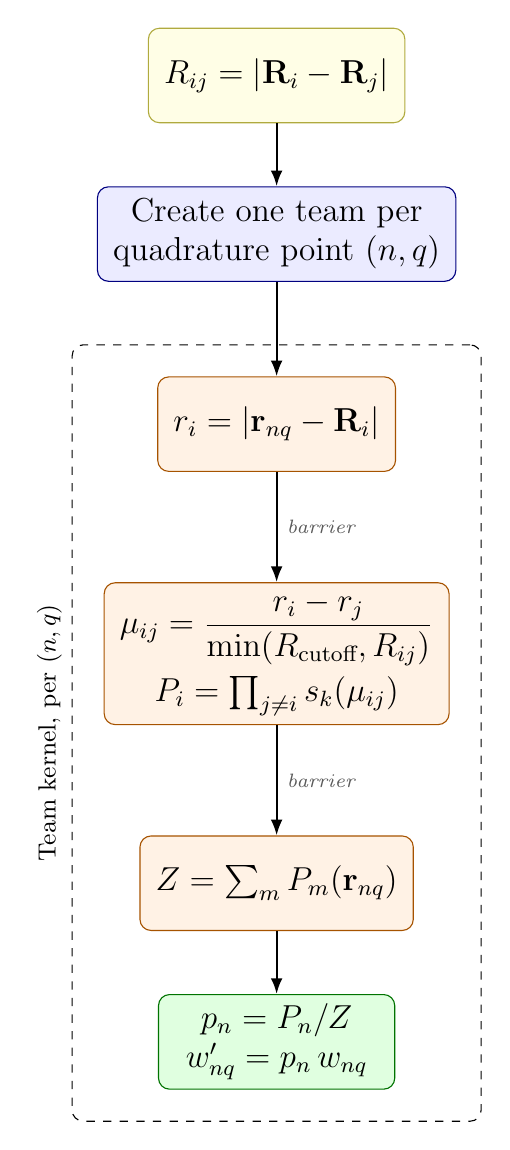
\begin{tikzpicture}[
        node distance=8mm,
        box/.style={draw, rounded corners,
          minimum height=12mm,
          minimum width= 30mm,
        align=center, font=\large, inner xsep=2mm},
        hostbox/.style={box, fill=blue!8,
        draw=blue!50!black},
        databox/.style={box, fill=yellow!10,
        draw=yellow!65!black},
        threadbox/.style={box,
        fill=orange!10, draw=orange!65!black},
        teambox/.style={box, fill=green!12,
        draw=green!45!black},
        arr/.style={-{Latex[length=2mm]}, thick},
        barrierlabel/.style={font=\scriptsize\itshape,
        text=gray!70!black}
      ]
      % Setup phase
      \node[databox] (dist) {
      $R_{ij} = | \mathbf R_i - \mathbf R_j|$};
      \node[hostbox, below=of dist] (policy)
      {Create one team per\\ quadrature point $(n,q)$};
      \draw[arr] (dist) -- (policy);
      % Team kernel phase
      \node[threadbox, below=12mm of policy] (cache)
      {$r_i = |\mathbf{r}_{nq} - \mathbf R_i|$};
      \node[threadbox, below=14mm of cache] (weights)
      {$\mu_{ij} = \dfrac{r_i - r_j}{\min(R_\text{cutoff},
        R_{ij})}$\\[1mm]
      $P_i = \prod_{j\neq i} s_k(\mu_{ij})$};
      \node[threadbox, below=14mm of weights] (reduce)
      {$Z = \sum_m P_m(\mathbf{r}_{nq})$};
      \node[teambox, below=of reduce] (write)
      {$p_n = P_n / Z$\\ $w'_{nq} = p_n\, w_{nq}$};
      \draw[arr] (policy) -- (cache);
      \draw[arr] (cache) -- (weights)
      node[midway, right, barrierlabel] {barrier};
      \draw[arr] (weights) -- (reduce)
      node[midway, right, barrierlabel] {barrier};
      \draw[arr] (reduce) -- (write);
      % Dashed team-kernel region, labelled down its side so the label costs
      % height rather than width.
      \begin{scope}[on background layer]
        \node[draw, dashed, rounded corners,
          fit=(cache)(weights)(reduce)(write),
          inner sep=4mm,
          label={[font=\small, rotate=90, anchor=south]left:{Team
        kernel, per $(n,q)$}}] {};
      \end{scope}
  \end{tikzpicture}}

  \vspace{6mm}

  % --- Table, full width ---
  {\small
    \begin{tabular}{@{}l l l l l@{}}
      \toprule
      Allocation & Type & Size & Symbol & Cache scope \\
      \midrule
      \texttt{atom\_centers}      &
      \texttt{View<Point*>}
      & $N_\text{nuc}$ &  $\mathbf{R}_i$            & --- \\
      \texttt{quadrature\_points} &
      \texttt{View<Point*>}
      & $N_\text{nuc}\cdot n_\text{quad}$ & $\mathbf{r}_{nq}$         & --- \\
      \texttt{weights}            &
      \texttt{View<double*>}
      & $N_\text{nuc}\cdot n_\text{quad}$   & $w_{nq} \to w'_{nq}$
      & --- \\
      \texttt{owner}            &
      \texttt{View<int*>}
      & $N_\text{nuc}\cdot n_\text{quad}$    & ---       & --- \\
      \texttt{R\_ij}              &
      \texttt{View<double**, RandomAccess>}
      & $N_\text{nuc}\times N_\text{nuc}$  & $R_{ij}$                  & --- \\
      \texttt{r\_cache}           &
      \texttt{View<double*,
      scratch\_memory\_space>} & $N_\text{nuc}$ & $r_i$
      & Per team \\
      \texttt{P\_cache}           &
      \texttt{View<double*,
      scratch\_memory\_space>} & $N_\text{nuc}$ & $P_i$
      & Per team \\
      \bottomrule
    \end{tabular}
    \captionof{table}{Memory allocations in
    \texttt{partition\_becke\_team}.}
  \label{tab:becke_team_memory_allocations}}

  \caption{Control-flow of the team-batched Becke partitioning
    routine, annotated
    with the underlying equations. Boxes are colored by
    execution scope: blue for
    host/serial setup, yellow for work distributed across
    GPU threads with data
    parallelism (via \texttt{Kokkos::RangePolicy}),
    orange for work distributed
    across GPU threads within a team (via
      \texttt{Kokkos::TeamVectorRange} or
    \texttt{Kokkos::TeamThreadRange}), and green for the
    single per-team write
  (via \texttt{Kokkos::single(PerTeam(\ldots))}).}
  \label{fig:becke_team_flow}
\end{figure}

Throughout this section \( n_\text{quad} \) denotes the number of
quadrature points generated per nucleus. The total number of quadrature
points, used in the remainder of this work, is therefore
\( N_\text{quad} = n_\text{quad} \cdot N_\text{nuc} \).

\subsection{Integral Routines}\label{subsec:integral_routines}

The integral routines computing the three- and two-center integrals of
the form $(\mu \nu|\alpha)$ and $(\alpha | \beta )$ are arguably
the most important implementations. We implemented two different
versions of each term contributing to the
Fock/Kohn--Sham matrix. The first relies
solely on dense linear algebra kernels and is therefore perfectly suited for
running on GPUs. The second relies on locally dense linear algebra
kernels and takes advantage of the local support of atom centered
orbitals. Each version comes with its specific advantages and
drawbacks, which we will analyze in the following subsections.

\subsubsection{Dense Linear Algebra RI-J and RI-K
schemes}\label{subsubsec:dense_la_rij_rik}

The dense linear algebra kernel relies on the idea that GPUs are
extremely good at doing dense general matrix-matrix (GEMM) and dense
general matrix-vector (GEMV) multiplications. Indeed, when applying
our quadrature rule given by \eqref{eq:global_quadrature} to
equations $\eqref{eq:coulomb-RI}$ and $\eqref{eq:exchange-RI}$ we can
rewrite them entirely with matrix-matrix multiplications. The schemes
we use to compute the Coulomb and the exchange matrices are commonly
known as the RI-J and RI-K schemes.

Since $\tilde J_{\mu \nu}$ and $\tilde K_{\mu \nu}$ both depend on
the density matrix $D_{\mu \nu }$, we need to recompute these
matrices during each SCF cycle. Nevertheless we are able to
pre-compute some quantities that can be reused within the schemes. We call
$\Phi_{\mu g} = \chi_\mu(\mathbf r_g)$ the basis collocation matrix,
$\tilde \Phi_{\alpha g} = \tilde \chi_\alpha(\mathbf r_g)$ the
auxiliary basis collocation matrix and
$\tilde V_{\alpha g} = \tilde V_\alpha(\mathbf r_g)$ the Coulomb
collocation matrix.

Another quantity which we can pre-compute is \( (\alpha | \beta )
^{-1} \). We proceed by first computing the overlap matrix in the
Coulomb metric

\begin{align}
  (\alpha | \beta )
  &= \int \tilde \chi _ {\alpha }(\mathbf r)
  \tilde{V}_\beta(\mathbf r)\mathrm d^3\mathbf r \\
  &= \sum_g w_g \tilde \chi _ {\alpha }(\mathbf r_g)
  \tilde{V}_\beta(\mathbf r_g) \\
  &= \sum_g w_g \tilde \Phi_{\alpha g}
  \tilde{V}_{\beta g}
\end{align}

and then use a singular value decomposition (SVD) to diagonalize the
matrix \( (\alpha | \beta ) = U S V^T = U S U^T\), where \( U \) and
\( V \) are orthonormal matrices and \( S \) is a diagonal matrix.
Since \( (\alpha | \beta ) \) is a symmetric positive definite matrix
we also know that \( U = V \).  We can then define the square-root
factor \( X^{\frac{1}{2}} = U S^{\frac{1}{2}} \) s.t. \(
X^{\frac{1}{2}}(X^{\frac{1}{2}})^T = (\alpha | \beta) \).
To enhance numerical stability we are also reducing the linear
dependence of the auxiliary basis functions by truncating the inner
dimension of the SVD to only contain the $K$ largest singular values.
Another way to think about this procedure is as a preconditioning
step, where we remove all singular values below a certain threshold
to lower the condition number of the inverted matrix. This procedure is known
as Löwdin's canonical orthogonalization.

The final inverse reads

\begin{align}
  (\alpha | \beta )^{-1}
  &= \sum_k (X^{-\frac{1}{2}})_{\alpha
  k}(X^{-\frac{1}{2}})_{\beta k }\\
  (X^{-\frac{1}{2}})_{\alpha k}
  &= U_{\alpha k} (S_k)^{-\frac{1}{2}}
\end{align}

Another, more computationally efficient, way to compute \(
X^{-\frac{1}{2}} \) is with a pivoted
Cholesky factorization of \( (\alpha | \beta  )\). We chose the SVD
method because the Cholesky factorization is, as of the writing of
this work, not implemented in the Kokkos Kernels library, whereas
third-party library calls of the SVD to LAPACK, CUDA and HIP exist natively in
Kokkos Kernels. One should
also note that the diagonalization step in the startup phase is negligible
compared to the overall SCF runtime.

Having precomputed all of the quantities above we are ready to tackle
the SCF cycles. During each SCF cycle we provide the Fock matrix to
an external SCF library, in our case we chose the reusable open source library
\texttt{OpenOrbitalOptimizer} \cite{Lehtola2025}. The SCF subroutine in
return provides us with the density matrix \( D_{\mu \nu } = \sum_i
f_i C_{\mu}^iC_{\nu }^i\), where \( f_i \) are the orbital occupation
numbers and \( C_{\mu}^i \) are the molecular-orbital coefficients
of the i-th occupied orbital. We then rebuild the Coulomb and
exchange contributions based on the new set of orbital coefficients.
For ease of notation we dropped the
dependence on the spin \( \sigma \), but in the case of an
unrestricted calculation we get one density matrix for each possible
spin value.

To avoid notation clutter we drop the upper bounds for
the summation indices. In all the following equations
\( (\mu,  \nu ,\lambda, \tau) \in [1,N_\text{bf}] \),
\( (\alpha,\beta) \in [1,N_\text{aux}] \),
\( g \in [1,N_{\text{quad}}] \),
\( i \in [1,N_{\text{occ}}] \),
\( k \in [1,K] \), where
\( N_\text{bf} \) is the number of basis functions in the
standard basis set,
\( N_\text{aux} \) is the number of basis functions in the
auxiliary basis set,
\( N_\text{quad} \) is the total number of quadrature points,
\( N_\text{occ} \) is the number of occupied orbitals and
\( K \) is the number of linearly independent auxiliary basis
functions, as explained above.

The RI-J scheme essentially tries to factorize the sums and collapse
the summation indices as
early as possible. To see how this is done we can rearrange the terms
in \eqref{eq:coulomb-RI} to obtain
\begin{equation}
  \tilde J_{\mu  \nu } = \sum_{\alpha}
  (\mu \nu | \alpha)\sum_{\beta}(\alpha |
  \beta)^{-1} \sum_{\lambda
  \tau}(\beta|\lambda\tau)D_{\lambda\tau}
  \label{eq:coulomb_rearranged}
\end{equation}

We can then compute a vector \( y \) that stores the
intermediate coefficients. We can do this efficiently by computing
the electron density \( \rho
\) on every quadrature point and doing a GEMV of \( \tilde V_{\beta
g} \) with \( (\rho_g w_g ) \).

\begin{align}
  y_\beta
  &= \sum_{\lambda
  \tau}(\beta|\lambda\tau)D^{\text{tot}}_{\lambda\tau}\\
  &= \int \sum_{\lambda \tau}
  \chi_\lambda(\mathbf{r})\chi_\tau(\mathbf{r})
  D^{\text{tot}}_{\lambda\tau} \tilde V_\beta(\mathbf{r})
  \mathrm d^3\mathbf{r}\\
  &= \int \rho(\mathbf r) \tilde V_\beta(\mathbf{r})
  \mathrm d^3\mathbf{r}\\
  &\approx   \sum_{g}\tilde{V}_\beta(\mathbf r_g) w
  (\mathbf r_g)\rho(\mathbf r_g) \\
  &= \sum_{g}\tilde{V}_{\beta g} w_g \rho_g
\end{align}

We then do two applications of \( X^{-\frac{1}{2}} \) via GEMV again
to obtain \( z_\alpha \).
\begin{align}
  z_\alpha
  = \sum_{\beta}(\alpha|\beta)^{-1}y_\beta
  \approx \sum_k (X^{-\frac{1}{2}})_{\alpha k} \sum_\beta
  (X^{-\frac{1}{2}})_{\beta k} \ y_\beta
\end{align}

We compute \( v_g =  \sum_{\alpha }
\tilde V_{\alpha g} z_\alpha  \) and scale the columns of \(
\Phi_{\mu g} \) by \( w_g v_g \). Finally we compute the result by
doing a GEMM of the scaled and the unscaled collocation matrices.

\begin{align}
  \tilde{J}_{\mu  \nu }
  &= \sum_{\alpha } (\mu \nu |\alpha ) z_\alpha \\
  &= \int \chi_\mu(\mathbf r) \chi_\nu(\mathbf r) \sum_{\alpha }
  \tilde V_\alpha(\mathbf r) z_\alpha \mathrm d^3 \mathbf r \\
  &\approx   \sum_{g}\chi_\mu(\mathbf{r}_g)
  \chi_\nu(\mathbf{r}_g) w(\mathbf{r}_g)  v(\mathbf{r}_g)\\
  &= \sum_g \Phi_{\mu g} w_g v_g \Phi_{\nu g}
\end{align}

This scheme has an asymptotic runtime of \( \mathcal O(N_\text{bf}^2 \times
N_\text{quad} )\) ( \( \approx \mathcal O(N_\text{bf}^3)\), if we assume that
\( N_\text{quad} \) scales linearly with \( N_\text{bf}  \)), where the
most expensive operation is the final GEMM.

The RI-K scheme is unfortunately not as factorizable as the RI-J
scheme, but we can still take advantage of the low-rank expansion of
the density matrix in order to get some factorizations. The
factorization then reads \( (\mu i | \alpha ) =  \sum_\lambda
C^i_{\lambda}(\mu \lambda |\alpha ) \). The RI-K scheme then boils
down to computing these 3-center integrals and applying \(
X^{-\frac{1}{2}} \) with a GEMM to obtain a matrix \( T^i_{\mu k} \).
We then perform a GEMM for each \( T^i_{\mu k} \) and scale the
result by \( f_i \), before adding the term to our final matrix.

\begin{align}
  \tilde K_{\mu  \nu }
  &= \sum_i f_i \sum_{\alpha \beta \lambda \tau}
  C_{\lambda}^i
  (\mu \lambda  | \alpha)(\alpha |
  \beta)^{-1} (\beta|\nu\tau) C_{\tau }^i \\
  &= \sum_i f_i \sum_{\alpha \beta }
  (\mu i | \alpha)(\alpha |
  \beta)^{-1} (\beta|\nu i)  \\
  &\approx \sum_i f_i \sum_{\alpha \beta }
  (\mu i | \alpha) \sum_k (X^{-\frac{1}{2}})_{\alpha k}
  (X^{-\frac{1}{2}})_{\beta k} (\beta|\nu i) \\
  &\approx \sum_i f_i \sum_k T^{i}_{\mu  k }  T^{i}_{\nu  k }
  \label{eq:exchange_rearranged}
\end{align}

The explicit computation of \( T^i_{\nu k } \) looks as follows
\begin{align}
  T^i_{\nu k }
  &=  \sum_\alpha (X^{-\frac{1}{2}})_{\alpha k}\, (\nu i | \alpha ) \\
  &=  \sum_\alpha (X^{-\frac{1}{2}})_{\alpha k}\, \int \chi_\nu(\mathbf r)
  \left(\sum_\lambda \chi_\lambda(\mathbf r)C_{\lambda}^i \right)
  \tilde V_\alpha(\mathbf r) \mathrm d^3 \mathbf r \\ 
  &= \sum_\alpha (X^{-\frac{1}{2}})_{\alpha k}\, \int
  \chi_\nu(\mathbf r) c^i(\mathbf r)
  \tilde V_\alpha(\mathbf r) \mathrm d^3 \mathbf r \\
  &\approx \sum_\alpha (X^{-\frac{1}{2}})_{\alpha k}\, \sum_g
  \Phi_{\nu g} w_ g c^{i}_{g}
  \tilde V_{\alpha g}
\end{align}

The most expensive operation being again a GEMM, but compared to the
RI-J scheme we need to do \( N_\text{occ} \) GEMMs. We end up with
a total asymptotic runtime of
\( \mathcal O(N_\text{occ} \times N_\text{bf}^2 \times
N_\text{quad}) \approx \mathcal O (N_\text{bf}^4) \).

Looking at this implementation we identify the GEMMs to be the
bottleneck. Given that we are planning to run on a GPU we are in an
ideal scenario since we have third-party library implementations
available to us in Kokkos Kernels, which are designed to be able to take full
advantage of our hardware.

The drawback of this implementation is its memory footprint. As stated
above, we pre-compute and store the basis collocation matrix
\(\Phi_{\mu g}\), the auxiliary collocation matrix \(\tilde\Phi_{\alpha g}\)
and the Coulomb collocation matrix \(\tilde V_{\alpha g}\). Each is a dense
matrix of size \(N_\text{bf}\times N_\text{quad}\) or
\(N_\text{aux}\times N_\text{quad}\), so the total number of stored
entries is \( M = (N_\text{bf} + 2\,N_\text{aux})\,N_\text{quad} \).

As a concrete example, we examine a moderately sized molecule with
\(N_\text{nuc}=100\) nuclei, a quadruple-\(\zeta\) Slater-type basis
(\(n_\text{bf}\approx 30\) functions per nucleus) with an auxiliary basis
of \(n_\text{aux}\approx 55\) functions per nucleus, and a medium-to-high
resolution grid of \(n_\text{quad}=10^4\) points per nucleus. This yields
\(N_\text{quad}=10^6\) quadrature points, so the basis collocation matrix
alone holds \(N_\text{bf}\times N_\text{quad}=3\times10^9\) entries, i.e.
\(24\,\text{GB}\) in double precision. Adding the two auxiliary matrices
(\(5.5\times10^9\) entries, \(44\,\text{GB}\) each) brings the collocation
data to roughly \(112\,\text{GB}\), well beyond the memory of a single GPU.
Since \(\tilde\Phi_{\alpha g}\) is only needed to assemble
\((\alpha|\beta)\) during setup, the persistent per-cycle footprint is
\(\Phi_{\mu g}\) and \(\tilde V_{\alpha g}\) (\(\approx 68\,\text{GB}\)).

The complete control-flow of the dense RI-J and RI-K routines, split
into the one-time startup phase and the operations repeated in every
SCF cycle, is summarized schematically in Figure
\ref{fig:dense_ri_flow}.

\begin{figure}[H]
  \centering
  % --- Vertical flowchart: the startup phase runs down the left, and the SCF
  % cycle runs top to bottom as two parallel branches (RI-J | RI-K) that
  % rejoin at the Fock assembly. ---
  \resizebox{\textwidth}{!}{%
    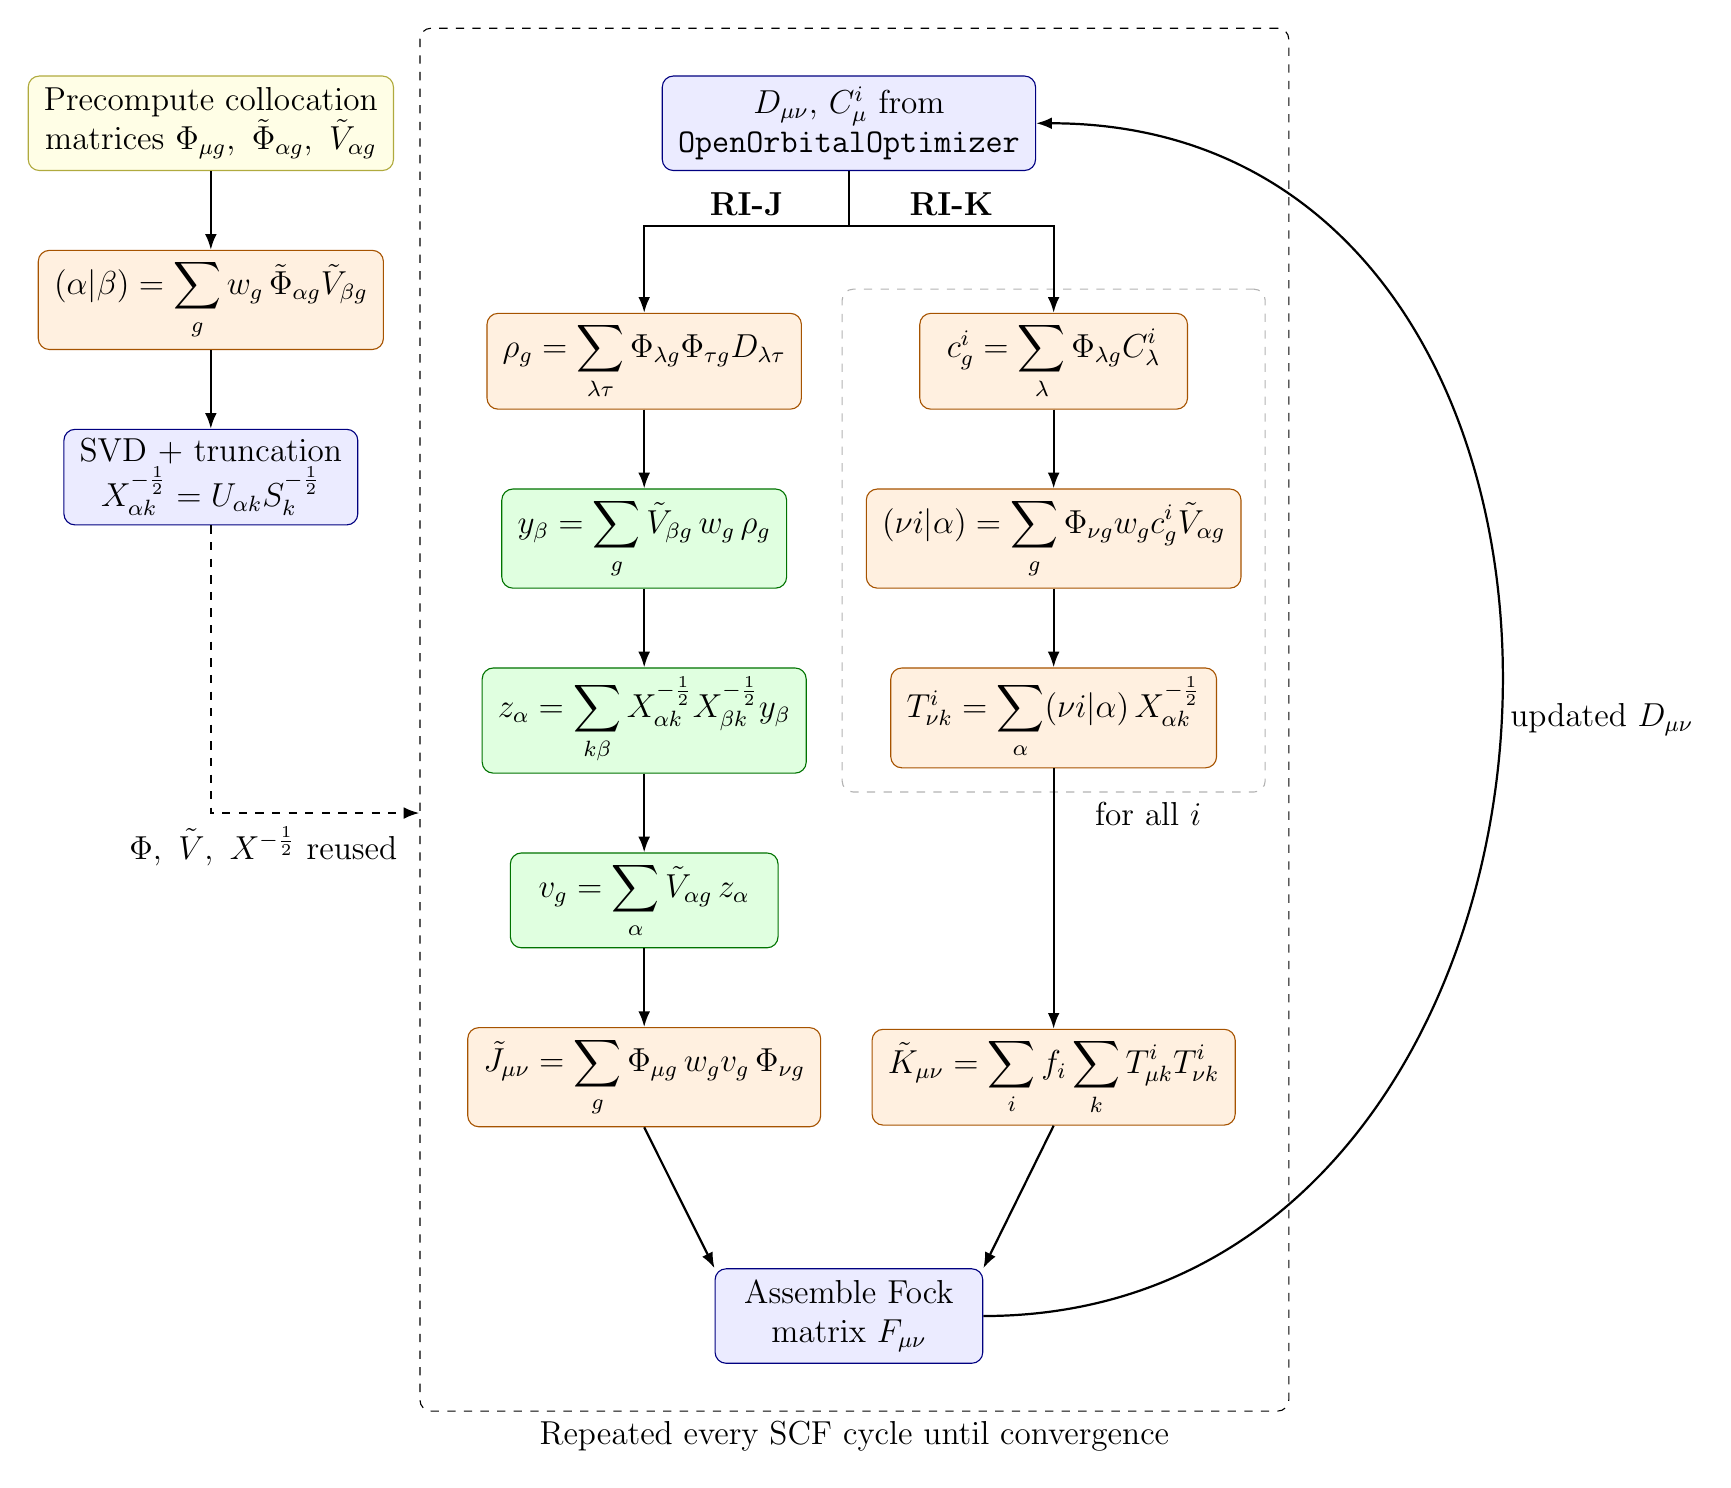
\begin{tikzpicture}[
        node distance=10mm,
        box/.style={draw, rounded corners,
          minimum height=12mm, minimum width=34mm,
        align=center, font=\large, inner xsep=2mm},
        hostbox/.style={box, fill=blue!8, draw=blue!50!black},
        databox/.style={box, fill=yellow!10, draw=yellow!65!black},
        gemmbox/.style={box, fill=orange!12, draw=orange!65!black},
        gemvbox/.style={box, fill=green!12, draw=green!45!black},
        arr/.style={-{Latex[length=2mm]}, thick},
        branchlabel/.style={font=\large\bfseries, text=black},
        looplabel/.style={font=\large, text=black!70!black}
      ]
      % --- Startup phase: its own column, top-left ---
      \node[databox] (colloc)
      {Precompute collocation\\matrices
      $\Phi_{\mu g},\ \tilde\Phi_{\alpha g},\ \tilde V_{\alpha g}$};
      \node[gemmbox, below=of colloc] (metric)
      {$(\alpha|\beta)=\displaystyle\sum_g w_g\,
      \tilde\Phi_{\alpha g}\tilde V_{\beta g}$};
      \node[hostbox, below=of metric] (svd)
      {SVD $+$ truncation\\
      $X^{-\frac12}_{\alpha k}=U_{\alpha k}S_k^{-\frac12}$};
      \draw[arr] (colloc) -- (metric);
      \draw[arr] (metric) -- (svd);

      % --- SCF entry, centred over the two branches ---
      \node[hostbox, right=34mm of colloc] (dens)
      {$D_{\mu\nu},\,C^i_\mu$ from\\\texttt{OpenOrbitalOptimizer}};

      % --- RI-J branch (left column) ---
      \node[gemmbox, below=18mm of dens, xshift=-26mm] (rho)
      {$\rho_g=\displaystyle\sum_{\lambda\tau}
      \Phi_{\lambda g}\Phi_{\tau g}D_{\lambda\tau}$};
      \node[gemvbox, below=of rho] (yb)
      {$y_\beta=\displaystyle\sum_g \tilde V_{\beta g}\,w_g\,\rho_g$};
      \node[gemvbox, below=of yb] (za)
      {$z_\alpha=\displaystyle\sum_{k\beta}
      X^{-\frac12}_{\alpha k}X^{-\frac12}_{\beta k}y_\beta$};
      \node[gemvbox, below=of za] (vg)
      {$v_g=\displaystyle\sum_\alpha \tilde V_{\alpha g}\,z_\alpha$};
      \node[gemmbox, below=of vg] (jmn)
      {$\tilde J_{\mu\nu}=\displaystyle\sum_g
      \Phi_{\mu g}\,w_g v_g\,\Phi_{\nu g}$};

      % --- RI-K branch (right column); K lands level with J ---
      \node[gemmbox, below=18mm of dens, xshift=26mm] (cig)
      {$c^i_g=\displaystyle\sum_\lambda \Phi_{\lambda g}C^i_\lambda$};
      \node[gemmbox, below=of cig] (mia)
      {$(\nu i|\alpha)=\displaystyle\sum_g
      \Phi_{\nu g}w_g c^i_g\tilde V_{\alpha g}$};
      \node[gemmbox, below=of mia] (tik)
      {$T^i_{\nu k}=\displaystyle\sum_\alpha
      (\nu i|\alpha)\,X^{-\frac12}_{\alpha k}$};
      \node[gemmbox] (kmn) at (cig |- jmn)
      {$\tilde K_{\mu\nu}=\displaystyle\sum_i f_i
      \sum_k T^i_{\mu k}T^i_{\nu k}$};

      % --- Fock assembly: where the two branches rejoin ---
      \node[hostbox, anchor=north]
      (fock) at ($(jmn.south)!0.5!(kmn.south)+(0,-18mm)$)
      {Assemble Fock \\matrix $F_{\mu\nu}$};

      % --- Arrows: split out of the density, rejoin at the Fock build ---
      \coordinate (split) at ($(dens.south)+(0,-7mm)$);
      \draw[thick] (dens.south) -- (split);
      \draw[arr] (split) -| (rho.north)
      node[pos=0.25, above, branchlabel] {RI-J};
      \draw[arr] (split) -| (cig.north)
      node[pos=0.25, above, branchlabel] {RI-K};
      \draw[arr] (rho) -- (yb);
      \draw[arr] (yb) -- (za);
      \draw[arr] (za) -- (vg);
      \draw[arr] (vg) -- (jmn);
      \draw[arr] (cig) -- (mia);
      \draw[arr] (mia) -- (tik);
      \draw[arr] (tik) -- (kmn);
      \draw[arr] (jmn.south) -- (fock.north west);
      \draw[arr] (kmn.south) -- (fock.north east);
      \draw[arr] (fock.east) to[out=0, in=0, looseness=1.4]
      node[midway, right, looplabel] {updated $D_{\mu\nu}$}
      (dens.east);

      % --- Background: dashed regions ---
      \begin{scope}[on background layer]
        \node[draw, dashed, rounded corners, inner sep=6mm,
          fit=(dens)(rho)(yb)(za)(vg)(jmn)(cig)(mia)(tik)(kmn)(fock),
          label={[looplabel]below:{Repeated every SCF cycle until
        convergence}}] (scf) {};
        \node[draw, dashed, rounded corners, draw=gray!60, inner sep=3mm,
          fit=(cig)(mia)(tik),
        label={[looplabel, xshift=12mm]below:{for all $i$}}] {};
      \end{scope}

      % --- Startup quantities reused each cycle. Routed down the left margin
      % and in between two branch rows, so the label sits in clear space
      % instead of on top of the SVD box. ---
      \coordinate (reuse) at ($(za.south)!0.5!(vg.north)$);
      \draw[arr, dashed] (svd.south) |- (scf.west |- reuse)
      node[pos=1, anchor=south east, yshift =-8mm , xshift=-1.5mm, looplabel]
      {$\Phi,\ \tilde V,\ X^{-\frac12}$ reused};
  \end{tikzpicture}}

  \caption{Control-flow of the dense RI-J and RI-K integral routines,
    annotated with the underlying equations. The boxes in the left-hand
    column form the one-time startup phase; everything inside the outer
    dashed region is re-evaluated in every SCF cycle, as two parallel
    branches that rejoin at the Fock build. Boxes are colored by
    operation type: blue for host orchestration and interaction with
    the external SCF library, yellow for pre-computed data held in
    device memory, orange for dense matrix--matrix products (GEMM), and
    green for matrix--vector products (GEMV) and element-wise scaling.
    The inner dashed box marks the loop over occupied orbitals in the
  RI-K scheme. The Fock/Kohn--Sham assembly is drawn schematically.}
  \label{fig:dense_ri_flow}
\end{figure}

\subsubsection{Dense Linear Algebra XC integrals}\label{subsubsec:dense_la_xc}

In order to do a DFT calculation we also need to compute the contributions
of the exchange-correlation (xc) functional to the Kohn--Sham matrix.
We will focus the discussion on our implementation of the functionals
that belong to the generalized gradient approximation level of theory;
the local density approximation is recovered as the special case of a
functional that does not depend on the density gradient, for which
\( \varepsilon_\gamma = 0 \) below and the gradient collocation
matrices are never needed. Our implementation closely follows the
algorithm described by Stocks and Barca~\cite{Stocks_2025}.

We write the xc energy as an integral over an energy density,
\begin{equation}
  E_\text{xc}^\text{GGA} = \int \varepsilon_\text{xc}^\text{GGA}
  \big(\rho(\mathbf r), \gamma(\mathbf r)\big)\,\mathrm d ^3 \mathbf r,
  \qquad \gamma(\mathbf r) = |\nabla \rho(\mathbf r)|^2,
  \label{eq:E_xc_gga}
\end{equation}
where \( \varepsilon_\text{xc}^\text{GGA} \) is the energy per unit
volume rather than per particle. With that convention the
abbreviations
\( \varepsilon_\rho = \partial \varepsilon_\text{xc}^\text{GGA} /
\partial \rho \) and
\( \varepsilon_\gamma = \partial \varepsilon_\text{xc}^\text{GGA} /
\partial \gamma \), used throughout this section, are precisely the two
quantities a functional library returns.

The contribution to the Kohn--Sham matrix reads \cite{Stocks_2025}
\begin{equation}
  V_{\mu \nu }^{\text{GGA}} = \frac{\partial
  E_\text{xc}^{\text{GGA}}}{\partial D_{\mu \nu }} =
  \int \Big( \chi_\mu(\mathbf r) Z_\nu(\mathbf r) + \chi_\nu(\mathbf r)
  Z_\mu(\mathbf r) \Big)\, \mathrm d ^3 \mathbf r,
  \label{eq:V_xc_gga}
\end{equation}

where \(  V_{\mu \nu }^{\text{GGA}}\) is the GGA version of
\(V^{xc}_{\mu\nu}\) from Equation~\eqref{eq:xc-matrix} and

\begin{equation}
  Z_\nu(\mathbf r) = \frac{1}{2} \chi_\nu(\mathbf r)
  \varepsilon_\rho(\mathbf r) + 2\big(\nabla \rho(\mathbf r)
  \cdot \nabla \chi_\nu(\mathbf r)\big)\, \varepsilon_\gamma(\mathbf r).
  \label{eq:Z_gga}
\end{equation}

Because of the symmetry of Equation~\eqref{eq:V_xc_gga} we need only
compute one term and symmetrize the result afterwards,

\begin{equation}
  V_{\mu \nu }^{\text{GGA}} = \bar V_{\mu \nu }^{\text{GGA}} +
  \bar V_{\nu \mu }^{\text{GGA}},
\end{equation}
where
\begin{equation}
  \bar V_{\mu \nu }^{\text{GGA}} = \int \chi_\mu(\mathbf r)
  Z_\nu(\mathbf r)\,  \mathrm d ^3 \mathbf r.
\end{equation}

Applying our quadrature schemes we obtain the following equations,
which we implemented again using the dense linear algebra routines
provided by the Kokkos Kernels library. Note that the dense scheme now
needs three more precomputed matrices,
\( \nabla_x\Phi_{\mu g} = \nabla_x\chi_{\mu}(\mathbf r_g) \),
\( \nabla_y\Phi_{\mu g} = \nabla_y\chi_{\mu}(\mathbf r_g) \) and
\( \nabla_z\Phi_{\mu g} = \nabla_z\chi_{\mu}(\mathbf r_g) \).

First we evaluate \( \rho \), \( \nabla\rho \) and \( \gamma  \) on the
grid. Differentiating \( \rho(\mathbf r) = \sum_{\lambda \tau}
D_{\lambda \tau}\chi_\lambda(\mathbf r)\chi_\tau(\mathbf r) \) produces
two terms that are equal by the symmetry of \( D \), which is where the
factor of two originates in equation \eqref{eq:diff_rho},

\begin{align}
  \rho_g &= \sum_{\lambda  \tau } \Phi_{\lambda g} \Phi_{\tau g}
  D_{\lambda  \tau}  \\
  \nabla_k\rho_g &= 2\sum_{\lambda  \tau } \nabla_k\Phi_{\lambda g}
  \Phi_{\tau g} D_{\lambda  \tau}, \qquad k \in \{x,y,z\} \label{eq:diff_rho} \\
  \gamma_g &= \nabla\rho_g \cdot \nabla\rho_g .
\end{align}

Evaluating these expressions as written would cost
\( \mathcal O(N_\text{bf}^2 \times N_\text{quad}) \). Since the density
is built from the occupied orbitals alone, we instead transform the
collocation matrices into the molecular orbital basis with four GEMMs,

\begin{equation}
  \Phi^\text{MO}_{i g} = \sum_\mu C_{\mu i}\Phi_{\mu g},
  \qquad
  \nabla_k\Phi^\text{MO}_{i g} = \sum_\mu C_{\mu i}\nabla_k\Phi_{\mu g},
\end{equation}

and contract over the occupied orbitals instead,

\begin{align}
  \rho_g &= \sum_i f_i \big(\Phi^\text{MO}_{i g}\big)^2 \\
  \nabla_k\rho_g &= 2\sum_i f_i \nabla_k\Phi^\text{MO}_{i g}
  \Phi^\text{MO}_{i g}.
\end{align}

The transforms scale as \( \mathcal O(N_\text{occ} \times N_\text{bf}
\times N_\text{quad}) \) and the contraction as \( \mathcal
O(N_\text{occ} \times N_\text{quad}) \), which is the same reduction we
already exploit in the RI-K scheme.

Then we pass \( \rho_g  \) and \( \gamma_g \) to
Libxc~\cite{Lehtola2018libxc}, which evaluates
\( \varepsilon_\rho(\mathbf r_g) \) and
\( \varepsilon_\gamma(\mathbf r_g)  \). Note that we have to evaluate
the functional on the CPU since we used Libxc Version 7.0.0 at the time of
writing the kernels. Libxc Version 7.1.0 is able to evaluate functionals
also on GPGPUs and we plan to implement kernels that do not have to
switch between GPGPU and CPU computations in future work.

We then move the evaluated functionals back to the GPU, where we
construct \( Z_{\mu g} \). We launch one team per quadrature point, and
each team launches one thread per basis function, so that each thread
computes one entry of \( Z_{\mu g} \). The quadrature weight is folded
in at this point, i.e. we store \( Z_{\mu g} = w_g Z_\mu(\mathbf r_g)
\), which avoids a separate pass to scale the collocation matrix.

Finally we perform one GEMM to compute
\begin{equation}
  \bar V_{\mu \nu } = \sum_g \Phi_{\mu g} Z_{\nu g}
\end{equation}

and symmetrize the result, \( V = \bar V + \bar V^T \).

A spin-unrestricted GGA functional depends on the two spin densities
\( \rho^\sigma \) and on the gradient invariants that can be built from
them,

\begin{equation}
  E_\text{xc}^\text{GGA} = \int \varepsilon_\text{xc}^\text{GGA}
  \big( \{\rho^\sigma\}, \{\gamma^{\sigma \sigma'}\} \big)\, \mathrm
  d^3 \mathbf r,
  \qquad
  \gamma^{\sigma \sigma'}(\mathbf r) = \nabla\rho^\sigma(\mathbf r)
  \cdot \nabla\rho^{\sigma'}(\mathbf r).
  \label{eq:E_xc_gga_polarized}
\end{equation}

Because the dot product is symmetric, \( \gamma^{\sigma \sigma'} =
\gamma^{\sigma' \sigma} \), only three of the four invariants are
independent, which is why a functional library exposes three of them.

Each spin channel now carries its own density matrix, so there is one
Kohn--Sham matrix per channel,
\( V^{\sigma}_{\mu \nu} = \partial E_\text{xc}^\text{GGA} / \partial
D^{\sigma}_{\mu \nu} \). Writing \( \sigma' \) for the opposite
channel, the chain rule runs over all five arguments of
\eqref{eq:E_xc_gga_polarized}, but two of them drop out: the opposite
spin density \( \rho^{\sigma'} \) does not depend on
\( D^{\sigma}_{\mu \nu} \), and neither does the invariant
\( \gamma^{\sigma' \sigma'} \), which is built from
\( \nabla \rho^{\sigma'} \) alone. Three terms therefore survive,

\begin{equation}
  V^{\sigma}_{\mu \nu} = \int \bigg(
    \varepsilon_{\rho^\sigma}
    \frac{\partial \rho^\sigma}{\partial D^{\sigma}_{\mu \nu}}
    + \varepsilon_{\gamma^{\sigma \sigma}}
    \frac{\partial \gamma^{\sigma \sigma}}{\partial D^{\sigma}_{\mu \nu}}
    + \varepsilon_{\gamma^{\sigma \sigma'}}
    \frac{\partial \gamma^{\sigma \sigma'}}{\partial D^{\sigma}_{\mu \nu}}
  \bigg)\, \mathrm d^3 \mathbf r,
  \label{eq:V_xc_chain_polarized}
\end{equation}

with \( \varepsilon_{\rho^\sigma} = \partial
\varepsilon_\text{xc}^\text{GGA} / \partial \rho^\sigma \) and
\( \varepsilon_{\gamma^{\sigma \sigma'}} = \partial
\varepsilon_\text{xc}^\text{GGA} / \partial \gamma^{\sigma \sigma'} \).
The three derivatives are

\begin{align}
  \frac{\partial \rho^\sigma}{\partial D^{\sigma}_{\mu \nu}}
  &= \chi_\mu \chi_\nu, \\
  \frac{\partial \gamma^{\sigma \sigma}}{\partial D^{\sigma}_{\mu \nu}}
  &= 2\, \nabla\rho^\sigma \cdot \nabla(\chi_\mu \chi_\nu), \\
  \frac{\partial \gamma^{\sigma \sigma'}}{\partial D^{\sigma}_{\mu \nu}}
  &= \nabla\rho^{\sigma'} \cdot \nabla(\chi_\mu \chi_\nu),
  \label{eq:gamma_derivatives}
\end{align}

where \( \nabla(\chi_\mu \chi_\nu) = \chi_\mu \nabla\chi_\nu + \chi_\nu
\nabla\chi_\mu \). The factor of two in the same-spin invariant appears
because \( \gamma^{\sigma \sigma} \) is quadratic in
\( \nabla \rho^\sigma \), whereas the cross invariant
\( \gamma^{\sigma \sigma'} \) is only linear in it and therefore carries
no such factor. This asymmetry is the one feature of the unrestricted
case that has no analogue in \eqref{eq:Z_gga}.

Substituting \eqref{eq:gamma_derivatives} into
\eqref{eq:V_xc_chain_polarized} and collecting the two gradient terms
into a single vector per channel,

\begin{equation}
  \mathbf v^\sigma(\mathbf r) = 2\, \varepsilon_{\gamma^{\sigma
  \sigma}}(\mathbf r)\, \nabla\rho^\sigma(\mathbf r)
  + \varepsilon_{\gamma^{\sigma \sigma'}}(\mathbf r)\,
  \nabla\rho^{\sigma'}(\mathbf r),
  \label{eq:v_sigma}
\end{equation}

gives

\begin{equation}
  V^{\sigma}_{\mu \nu} = \int \Big( \varepsilon_{\rho^\sigma}
    \chi_\mu \chi_\nu + \mathbf v^\sigma \cdot
  \nabla(\chi_\mu \chi_\nu) \Big)\, \mathrm d^3 \mathbf r,
\end{equation}

which has exactly the structure of the restricted expression and can be
split the same way, \( V^{\sigma}_{\mu \nu} = \bar{V}^{\sigma}_{\mu
\nu} + \bar V^{\sigma}_{\nu \mu} \), with

\begin{equation}
  Z^\sigma_\nu(\mathbf r) = \frac{1}{2} \chi_\nu(\mathbf r)\,
  \varepsilon_{\rho^\sigma}(\mathbf r) + \mathbf v^\sigma(\mathbf r)
  \cdot \nabla \chi_\nu(\mathbf r).
  \label{eq:Z_gga_polarized}
\end{equation}

Comparing \eqref{eq:Z_gga_polarized} with \eqref{eq:Z_gga} shows that
the restricted scheme is recovered by setting \( \mathbf v = 2
\varepsilon_\gamma \nabla\rho \), i.e. by dropping the cross term.

We evaluate \( \rho^\sigma \) and
\( \nabla\rho^\sigma \) once per channel with the orbital-based
contraction above, form the three invariants, and interleave them into
the layout the library expects, which stores the two densities and the
three invariants consecutively per grid point. A single call then
returns \( \varepsilon_{\rho^\sigma} \) and
\( \varepsilon_{\gamma^{\sigma \sigma'}} \) for every grid point, which
we de-interleave and use to build the two vectors
\eqref{eq:v_sigma} in one pass over the grid. From that point on the
two channels are independent: the kernel that builds \( Z^\sigma_{\mu g}
\), the GEMM and the symmetrization are the same routine as in the
restricted case, invoked once per channel with its own
\( \varepsilon_{\rho^\sigma} \) and \( \mathbf v^\sigma \). Only the
construction of \( \mathbf v^\sigma \) is new, so the unrestricted path
costs one extra grid pass and a second assembly.

The complete control-flow of the unrestricted routine is summarized in
Figure~\ref{fig:gga_lsda_flow} and all memory allocations are listed in
Table~\ref{tab:gga_lsda_memory}.

\begin{figure}[H]
  \centering
  % --- Vertical flowchart. The two spin channels run as parallel columns
  % that join twice: once to form the cross invariant and call the
  % functional, and once more for the energy. ---
  \resizebox{!}{0.74\textheight}{%
    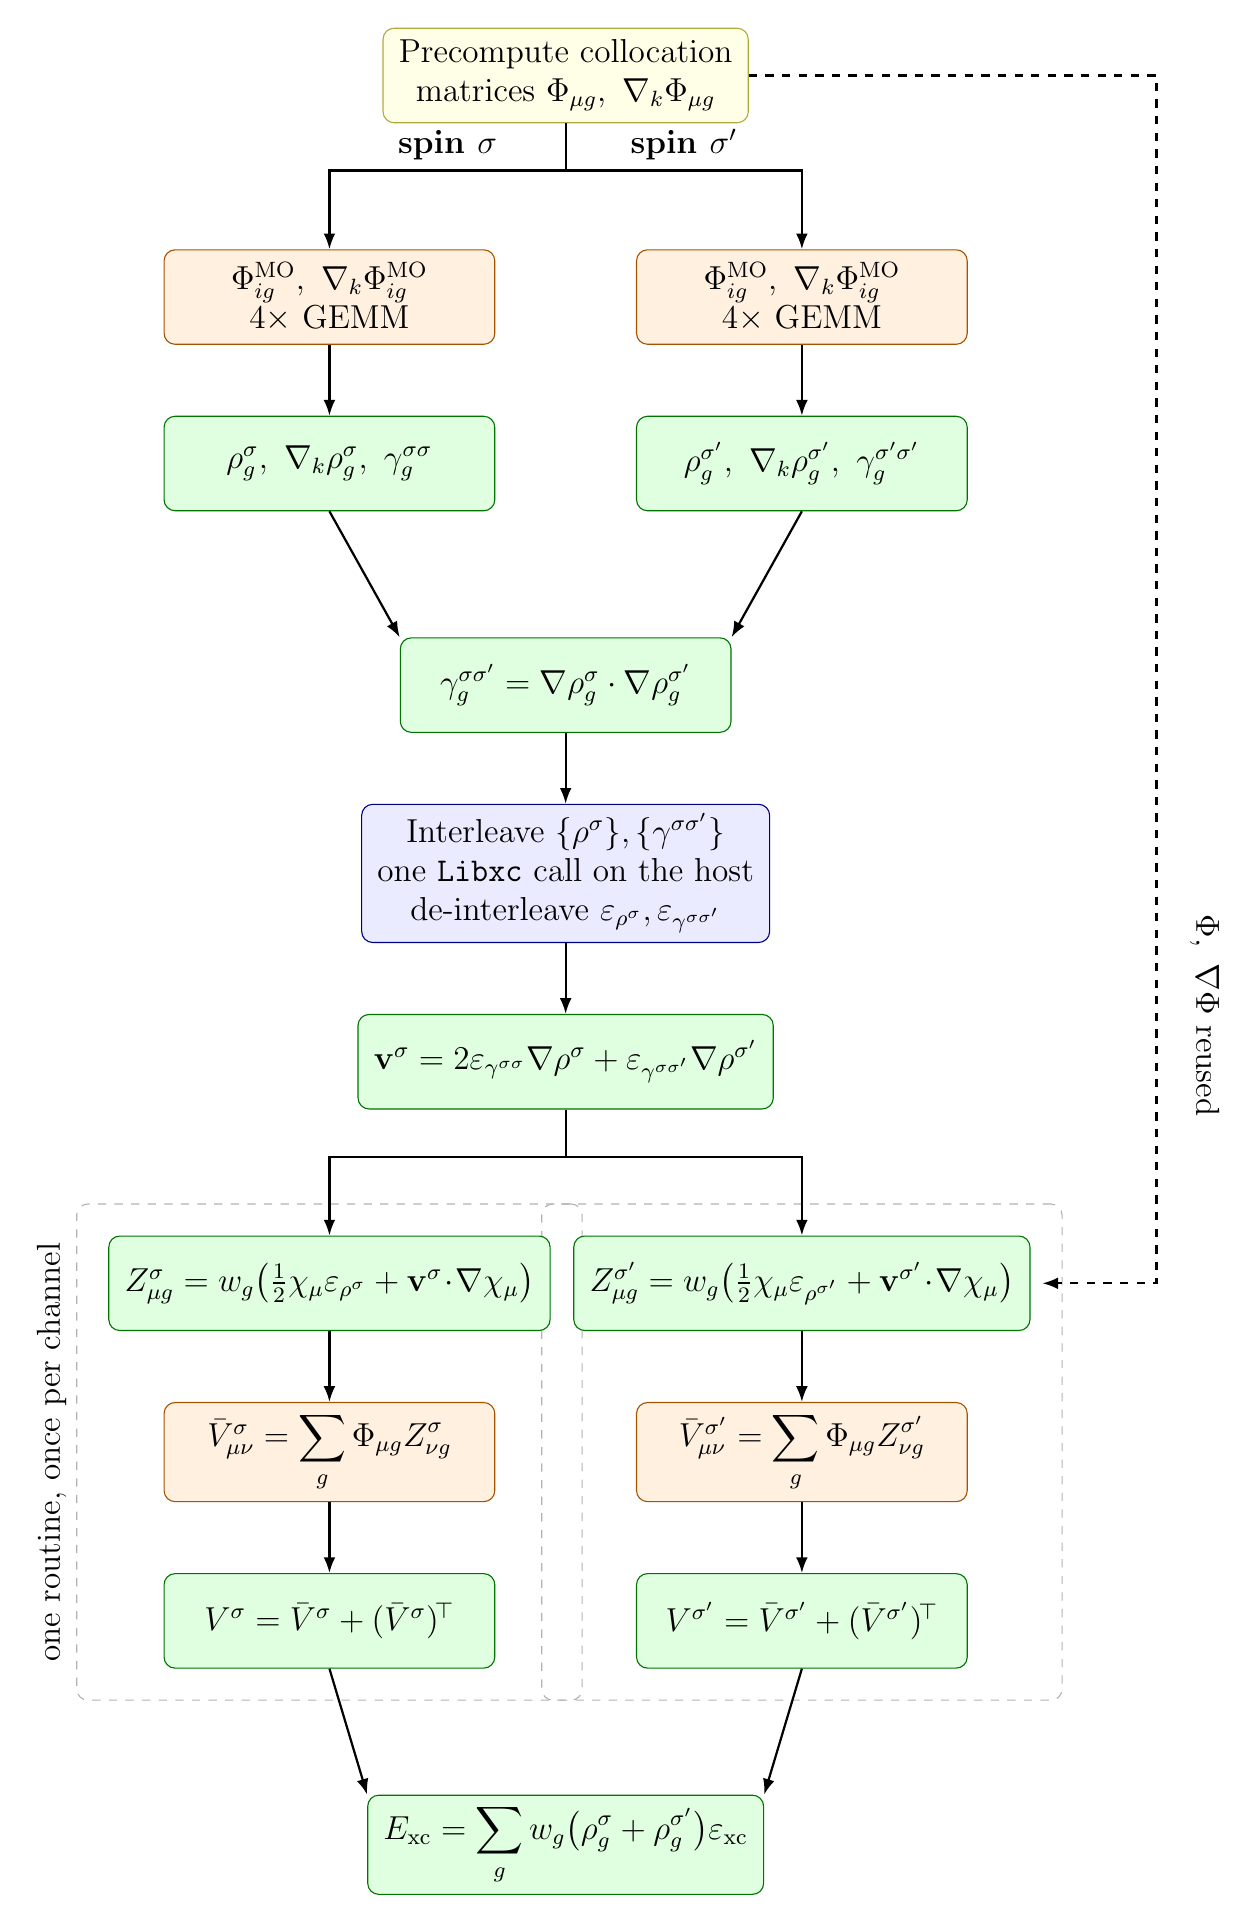
\begin{tikzpicture}[
        node distance=9mm,
        box/.style={draw, rounded corners,
          minimum height=12mm, minimum width=42mm,
        align=center, font=\large, inner xsep=2mm},
        hostbox/.style={box, fill=blue!8, draw=blue!50!black},
        databox/.style={box, fill=yellow!10, draw=yellow!65!black},
        gemmbox/.style={box, fill=orange!12, draw=orange!65!black},
        teambox/.style={box, fill=green!12, draw=green!45!black},
        arr/.style={-{Latex[length=2mm]}, thick},
        branchlabel/.style={font=\large\bfseries, text=black},
        looplabel/.style={font=\large, text=black!70!black}
      ]
      % --- Startup data, shared by both channels ---
      \node[databox] (colloc)
      {Precompute collocation\\matrices
      $\Phi_{\mu g},\ \nabla_k\Phi_{\mu g}$};

      % --- Channel columns ---
      \node[gemmbox, below=16mm of colloc, xshift=-30mm] (moa)
      {$\Phi^\text{MO}_{ig},\ \nabla_k\Phi^\text{MO}_{ig}$\\$4\times$ GEMM};
      \node[gemmbox, below=16mm of colloc, xshift=30mm] (mob)
      {$\Phi^\text{MO}_{ig},\ \nabla_k\Phi^\text{MO}_{ig}$\\$4\times$ GEMM};
      \node[teambox, below=of moa] (dena)
      {$\rho^\sigma_g,\ \nabla_k\rho^\sigma_g,\
      \gamma^{\sigma\sigma}_g$};
      \node[teambox, below=of mob] (denb)
      {$\rho^{\sigma'}_g,\ \nabla_k\rho^{\sigma'}_g,\
      \gamma^{\sigma'\sigma'}_g$};

      % --- First join: cross invariant, then the functional on the host ---
      \node[teambox, anchor=north]
      (cross) at ($(dena.south)!0.5!(denb.south)+(0,-16mm)$)
      {$\gamma^{\sigma\sigma'}_g=\nabla\rho^\sigma_g\cdot
      \nabla\rho^{\sigma'}_g$};
      \node[hostbox, below=of cross] (libxc)
      {Interleave $\{\rho^\sigma\},\{\gamma^{\sigma\sigma'}\}$\\
        one \texttt{Libxc} call on the host\\
        de-interleave $\varepsilon_{\rho^\sigma},
      \varepsilon_{\gamma^{\sigma\sigma'}}$};
      \node[teambox, below=of libxc] (vfield)
      {$\mathbf v^\sigma=2\varepsilon_{\gamma^{\sigma\sigma}}
        \nabla\rho^\sigma+\varepsilon_{\gamma^{\sigma\sigma'}}
      \nabla\rho^{\sigma'}$};

      % --- Second split: per-channel assembly, identical routine ---
      \node[teambox, below=16mm of vfield, xshift=-30mm] (za)
      {$Z^\sigma_{\mu g}=w_g\big(\tfrac12\chi_\mu
      \varepsilon_{\rho^\sigma}+\mathbf v^\sigma\!\cdot\!\nabla\chi_\mu\big)$};
      \node[teambox, below=16mm of vfield, xshift=30mm] (zb)
      {$Z^{\sigma'}_{\mu g}=w_g\big(\tfrac12\chi_\mu
          \varepsilon_{\rho^{\sigma'}}+\mathbf v^{\sigma'}\!\cdot\!
      \nabla\chi_\mu\big)$};
      \node[gemmbox, below=of za] (va)
      {$\bar V^\sigma_{\mu\nu}=\displaystyle\sum_g
      \Phi_{\mu g}Z^\sigma_{\nu g}$};
      \node[gemmbox, below=of zb] (vb)
      {$\bar V^{\sigma'}_{\mu\nu}=\displaystyle\sum_g
      \Phi_{\mu g}Z^{\sigma'}_{\nu g}$};
      \node[teambox, below=of va] (syma)
      {$V^\sigma=\bar V^\sigma+(\bar V^\sigma)^{\!\top}$};
      \node[teambox, below=of vb] (symb)
      {$V^{\sigma'}=\bar V^{\sigma'}+(\bar V^{\sigma'})^{\!\top}$};

      % --- Second join: the energy ---
      \node[teambox, anchor=north]
      (energy) at ($(syma.south)!0.5!(symb.south)+(0,-16mm)$)
      {$E_\text{xc}=\displaystyle\sum_g w_g
        \big(\rho^\sigma_g+\rho^{\sigma'}_g\big)
      \varepsilon_\text{xc}$};

      % --- Arrows ---
      \coordinate (split1) at ($(colloc.south)+(0,-6mm)$);
      \draw[thick] (colloc.south) -- (split1);
      \draw[arr] (split1) -| (moa.north)
      node[pos=0.25, above, branchlabel] {spin $\sigma$};
      \draw[arr] (split1) -| (mob.north)
      node[pos=0.25, above, branchlabel] {spin $\sigma'$};
      \draw[arr] (moa) -- (dena);
      \draw[arr] (mob) -- (denb);
      \draw[arr] (dena.south) -- (cross.north west);
      \draw[arr] (denb.south) -- (cross.north east);
      \draw[arr] (cross) -- (libxc);
      \draw[arr] (libxc) -- (vfield);
      \coordinate (split2) at ($(vfield.south)+(0,-6mm)$);
      \draw[thick] (vfield.south) -- (split2);
      \draw[arr] (split2) -| (za.north);
      \draw[arr] (split2) -| (zb.north);
      \draw[arr] (za) -- (va);
      \draw[arr] (zb) -- (vb);
      \draw[arr] (va) -- (syma);
      \draw[arr] (vb) -- (symb);
      \draw[arr] (syma.south) -- (energy.north west);
      \draw[arr] (symb.south) -- (energy.north east);

      % --- The per-channel assembly is one routine, called twice ---
      \begin{scope}[on background layer]
        \node[draw, dashed, rounded corners, draw=gray!60, inner sep=4mm,
          fit=(za)(va)(syma),
          label={[looplabel, rotate=90, anchor=south]left:{one routine,
        once per channel}}] {};
        \node[draw, dashed, rounded corners, draw=gray!60, inner sep=4mm,
        fit=(zb)(vb)(symb)] {};
      \end{scope}

      % --- Collocation matrices are reused by the Z kernels ---
      \coordinate (reusex) at ($(zb.east)+(16mm,0)$);
      \draw[arr, dashed, shorten >=1.5mm] (colloc.east) -| (reusex)
      -- (zb.east);
      \node[looplabel, rotate=-90, anchor=south]
      at ($(reusex)+(3mm,34mm)$) {$\Phi,\ \nabla\Phi$ reused};
  \end{tikzpicture}}

  \caption{Control-flow of the spin-unrestricted GGA routine
    \texttt{compute\_gga\_lsda}, annotated with the underlying
    equations. The two spin channels run as parallel columns and join
    twice: once to form the cross invariant
    $\gamma^{\sigma\sigma'}$, which is the only quantity that couples
    them, and once at the end for the energy. Boxes are colored by
    operation type: blue for host-side orchestration and the functional
    evaluation, which has to run on the CPU; yellow for pre-computed
    data held in device memory; orange for dense matrix--matrix
    products (GEMM); and green for team-parallel kernels over the
    quadrature grid. The two dashed regions mark the per-channel
    assembly, which is a single routine invoked once per spin with its
    own $\varepsilon_{\rho^\sigma}$ and $\mathbf v^\sigma$: only the
    construction of $\mathbf v^\sigma$ above it is specific to the
  unrestricted case.}
  \label{fig:gga_lsda_flow}
\end{figure}

\begin{table}[H]
  \centering
  {\small
    \begin{tabular}{@{}llllc@{}}
      \toprule
      Allocation & Type & Size & Symbol & Space \\
      \midrule
      \texttt{rho\_\{a,b\}}         & \texttt{View<double*>}
      & $N_\text{quad}$ & $\rho^\sigma_g$ & device \\
      \texttt{g\{x,y,z\}\{a,b\}}    & \texttt{View<double*>}
      & $N_\text{quad}$ & $\nabla_k\rho^\sigma_g$ & device \\
      \texttt{sigma\_\{aa,bb\}}     & \texttt{View<double*>}
      & $N_\text{quad}$ & $\gamma^{\sigma\sigma}_g$ & device \\
      \texttt{sigma\_ud}            & \texttt{View<double*>}
      & $N_\text{quad}$ & $\gamma^{\sigma\sigma'}_g$ & device \\
      \midrule
      \texttt{rho\_pol\_h}          & \texttt{View<double*, Host>}
      & $2N_\text{quad}$ & $\{\rho^\sigma_g\}$ interleaved & host \\
      \texttt{sigma\_pol\_h}        & \texttt{View<double*, Host>}
      & $3N_\text{quad}$ & $\{\gamma^{\sigma\sigma'}_g\}$ interleaved & host \\
      \texttt{vrho\_pol\_h}         & \texttt{View<double*, Host>}
      & $2N_\text{quad}$ & $\{\varepsilon_{\rho^\sigma}\}$ interleaved & host \\
      \texttt{vsigma\_pol\_h}       & \texttt{View<double*, Host>}
      & $3N_\text{quad}$
      & $\{\varepsilon_{\gamma^{\sigma\sigma'}}\}$ interleaved & host \\
      \texttt{exc\_h}               & \texttt{View<double*, Host>}
      & $N_\text{quad}$ & $\varepsilon_\text{xc}$ & host \\
      \midrule
      \texttt{exc}                  & \texttt{View<double*>}
      & $N_\text{quad}$ & $\varepsilon_\text{xc}$ & device \\
      \texttt{vrho\_\{up,down\}}    & \texttt{View<double*>}
      & $N_\text{quad}$ & $\varepsilon_{\rho^\sigma}$ & device \\
      \texttt{vsigma\_\{uu,ud,dd\}} & \texttt{View<double*>}
      & $N_\text{quad}$ & $\varepsilon_{\gamma^{\sigma\sigma'}}$ & device \\
      \texttt{vec\{x,y,z\}\_\{up,dn\}} & \texttt{View<double*>}
      & $N_\text{quad}$ & $\mathbf v^\sigma$ & device \\
      \midrule
      \texttt{Z}                    & \texttt{View<double**>}
      & $N_\text{bf}\times N_\text{quad}$ & $Z^\sigma_{\mu g}$ & device \\
      \texttt{V}, \texttt{V\_result} & \texttt{View<double**>}
      & $N_\text{bf}\times N_\text{bf}$ & $\bar V^\sigma,\ V^\sigma$ & device \\
      \bottomrule
  \end{tabular}}
  \caption{Memory allocations in \texttt{compute\_gga\_lsda}. All device
    views use \texttt{Kokkos::LayoutLeft}. The last two rows are
    allocated inside
    the per-channel assembly and therefore exist once per spin. The
    dominant term is $\texttt{Z}$, which matches the collocation matrix
    in size, so the unrestricted GGA build costs one extra
    $N_\text{bf}\times N_\text{quad}$ array on top of the four
    collocation matrices it reads; everything else scales with
    $N_\text{quad}$ alone. The interleaved host buffers are required by
    the functional library's spin-polarized calling
  convention.}
  \label{tab:gga_lsda_memory}
\end{table}

\subsubsection{Locally Dense Linear
Algebra}\label{subsubsec:locally_dense_la}

The locally dense linear algebra implementation of the RI-J and RI-K
schemes tries to overcome the drawbacks of the dense schemes by not
pre-computing the collocation matrices but instead recomputing them
during each SCF cycle. Recomputing the collocation matrices allows us
to take advantage of atomic orbitals locality.

Atomic orbitals are almost always designed in a way that their radial
function decays at least exponentially far away from their originating
nucleus. This exponential decay lets us define a cutoff radius,
after which the contributions to the integrals become negligible.
Concretely, we do not need to evaluate all basis functions at
every quadrature point; instead we perform a pre-screening
step, where we compute a neighbor list, which matches basis functions to
sets of quadrature points.

The construction of the neighbor list proceeds in the following
steps. First, we create bounding boxes around points that are close to
each other in space, i.e. we want to find clusters of points. Second,
we compute bounding boxes around those clusters. Third, we compute a
cutoff radius for each basis function. Lastly, we compute the
intersection of all spheres, generated by taking the origin of a basis
function as the center and the cutoff radius as the radius, with all
bounding boxes. If a sphere intersects a bounding box we add it to the
neighbor list.

Fortunately there exists a reusable open source library, called
\texttt{ArborX} \cite{LebrunGrandie2020, Prokopenko2025}, written
entirely in Kokkos, which we are able to
seamlessly integrate into our routines. Through \texttt{ArborX}'s API
we reorder our quadrature points according to a Z-order. The Z-order
relies on a space filling curve, which on average makes points that
are close to each other in space, also close to each other in
hardware memory. We then build bounding boxes around a pre-defined
number of points, i.e. a box of size \( N_B \) contains exactly \( N_B \)
points. Since we previously ordered our points, we simply define one
box to contain all points with indices \( i \in [nN_B+1, (n+1)N_B]
\). To define the cutoff radii \(  r_\text{cutoff} \) we use a
screening threshold \( \tau_\text{cutoff} \), s.t.
\( r > r_\text{cutoff} \implies B(r) < \tau_\text{cutoff} \).
Lastly, providing \texttt{ArborX} with the
bounding boxes and cutoff radii, it returns the neighbor list.

In the locally dense scheme the RI-J and RI-K algorithms keep the same
structure as their dense counterparts; the difference is that every
operation whose inner dimension was the full set of quadrature points is
replaced by a custom team-batched kernel that only visits the points and
basis functions retained by the neighbor list. We launch one Kokkos team
per box and, following the same hierarchical-parallelism pattern as the
Becke partitioning routine (Figure~\ref{fig:becke_team_flow}), stage the
basis-function evaluations \( \chi_\mu(\mathbf r_g) \) through a fixed-size
neighbor-tile cache in team scratch memory.

The tiled RI-J routine runs as two team kernels separated by a host-side
application of \( (\alpha|\beta)^{-1} \): the first accumulates the
fitted-density coefficients \( y_\alpha \) (rescaled to \( z_\alpha \) by
two GEMVs), the second contracts the fitted potential back onto basis
pairs to assemble \( \tilde J_{\mu\nu} \). Its control-flow is shown in
Figure~\ref{fig:tiled_rij_flow} and its allocations in
Table~\ref{tab:tiled_rij_memory}. The tiled RI-K routine loops over the
occupied orbitals: for each orbital \( i \) it folds \( c^i(\mathbf r_g)
=\sum_\lambda C^i_\lambda \chi_\lambda(\mathbf r_g) \) into the
quadrature weights, builds
the half-transformed three-center integral \( (\nu i|\alpha) \) with the
tiled kernel -- evaluating every neighbor tile of \( \chi_\nu \) once and
reusing it across all auxiliary functions \( \alpha \) -- and then
applies \( X^{-\frac12} \) and accumulates \( \tilde K_{\mu\nu} \) with
two GEMMs. Its control-flow and allocations are given in
Figure~\ref{fig:tiled_rik_flow} and Table~\ref{tab:tiled_rik_memory}.

\begin{figure}[H]
  \centering
  \resizebox{\textwidth}{!}{%
    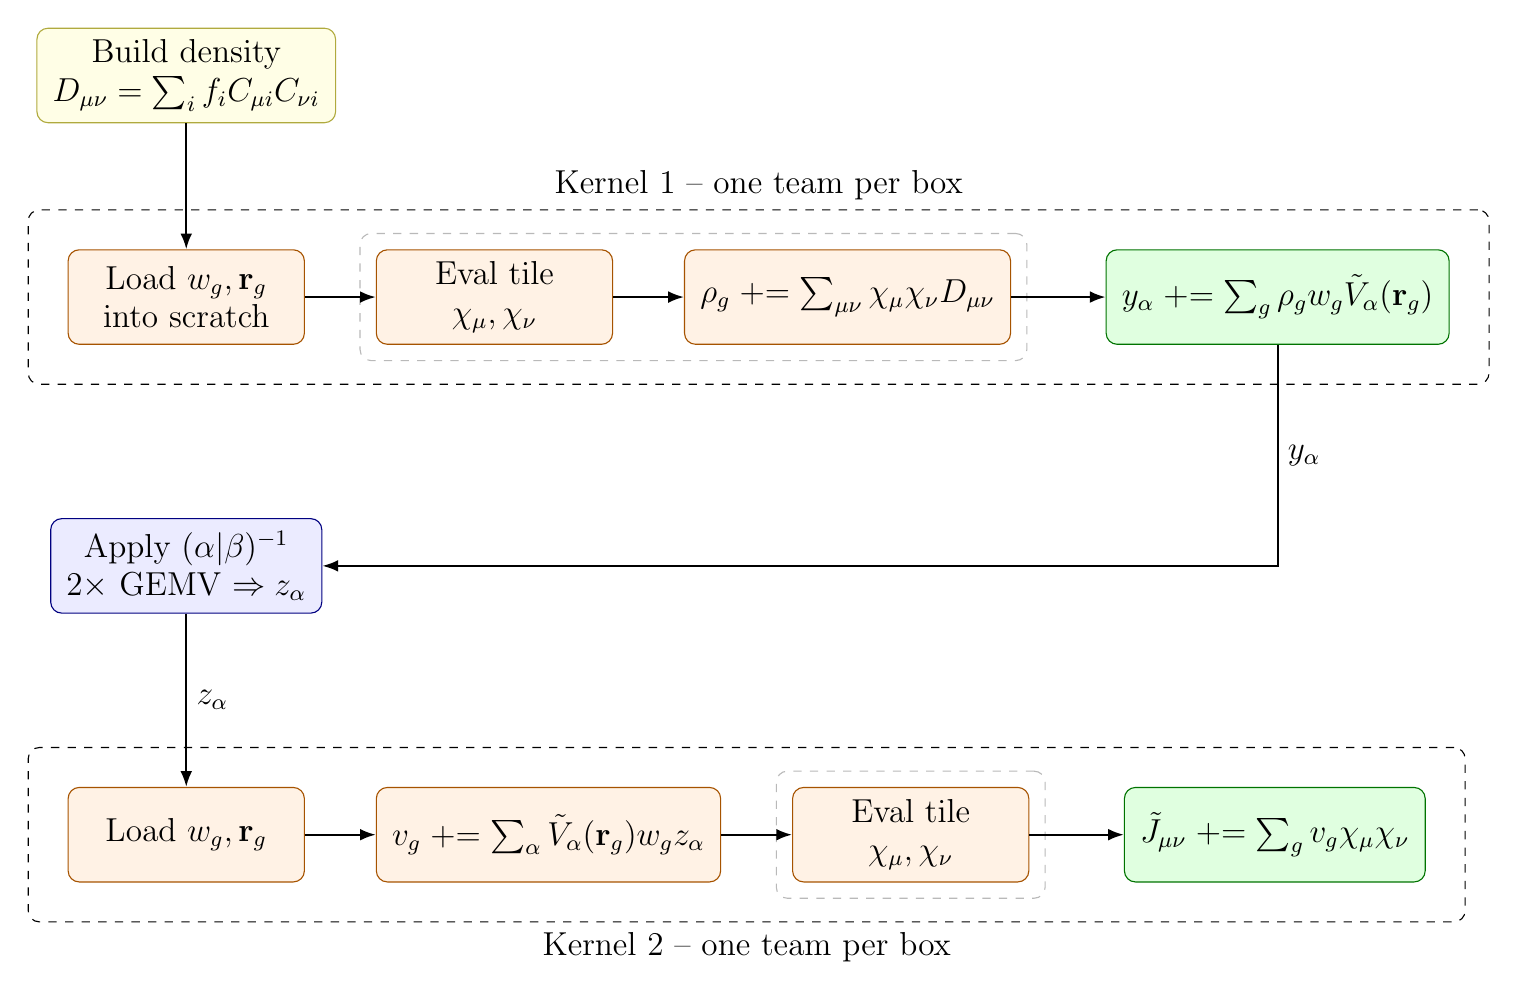
\begin{tikzpicture}[
        node distance=9mm,
        box/.style={draw, rounded corners, minimum height=12mm,
        minimum width=30mm, align=center, font=\large, inner xsep=2mm},
        hostbox/.style={box, fill=blue!8, draw=blue!50!black},
        databox/.style={box, fill=yellow!10, draw=yellow!65!black},
        threadbox/.style={box, fill=orange!10, draw=orange!65!black},
        teambox/.style={box, fill=green!12, draw=green!45!black},
        arr/.style={-{Latex[length=2mm]}, thick},
        looplabel/.style={font=\large, text=black!70!black}
      ]
      \node[databox] (dbuild)
      {Build density\\$D_{\mu\nu}=\sum_i f_i C_{\mu i}C_{\nu i}$};
      \node[threadbox, below=16mm of dbuild] (load1)
      {Load $w_g,\mathbf r_g$\\into scratch};
      \node[threadbox, right=of load1] (phi1) {Eval
      tile\\$\chi_\mu,\chi_\nu$};
      \node[threadbox, right=of phi1] (rho)
      {$\rho_g\mathrel{+}=\sum_{\mu\nu}\chi_\mu\chi_\nu D_{\mu\nu}$};
      \node[teambox, right=12mm of rho] (yalpha)
      {$y_\alpha\mathrel{+}=\sum_g \rho_g w_g \tilde
      V_\alpha(\mathbf r_g)$};
      \node[hostbox, below=22mm of load1] (inv)
      {Apply $(\alpha|\beta)^{-1}$\\$2\times$ GEMV $\Rightarrow z_\alpha$};
      \node[threadbox, below=22mm of inv] (load2) {Load $w_g,\mathbf r_g$};
      \node[threadbox, right=of load2] (vbuild)
      {$v_g\mathrel{+}=\sum_\alpha \tilde V_\alpha(\mathbf r_g)
      w_g z_\alpha$};
      \node[threadbox, right=of vbuild] (phi2) {Eval
      tile\\$\chi_\mu,\chi_\nu$};
      \node[teambox, right=12mm of phi2] (jij)
      {$\tilde J_{\mu\nu}\mathrel{+}=\sum_g v_g \chi_\mu\chi_\nu$};
      \draw[arr] (dbuild) -- (load1);
      \draw[arr] (load1) -- (phi1);
      \draw[arr] (phi1) -- (rho);
      \draw[arr] (rho) -- (yalpha);
      \draw[arr] (yalpha.south) |- (inv.east)
      node[near start, right, looplabel] {$y_\alpha$};
      \draw[arr] (inv) -- (load2) node[midway, right, looplabel]
      {$z_\alpha$};
      \draw[arr] (load2) -- (vbuild);
      \draw[arr] (vbuild) -- (phi2);
      \draw[arr] (phi2) -- (jij);
      \begin{scope}[on background layer]
        \node[draw, dashed, rounded corners, inner sep=5mm,
          fit=(load1)(phi1)(rho)(yalpha),
        label={[looplabel]above:{Kernel 1 -- one team per box}}] {};
        \node[draw, dashed, rounded corners, inner sep=5mm,
          fit=(load2)(vbuild)(phi2)(jij),
        label={[looplabel]below:{Kernel 2 -- one team per box}}] {};
        \node[draw, dashed, draw=gray!55, rounded corners, inner sep=2mm,
        fit=(phi1)(rho)] {};
        \node[draw, dashed, draw=gray!55, rounded corners, inner sep=2mm,
        fit=(phi2)] {};
      \end{scope}
  \end{tikzpicture}}
  \caption{Control-flow of the neighbor-tiled RI-J kernel
    (\texttt{compute\_coulomb\_tiled}). One Kokkos team is launched per
    neighbor-list box. Kernel~1 accumulates the fitted-density
    coefficients $y_\alpha$; a host-side application of
    $(\alpha|\beta)^{-1}$ (two GEMVs) rescales them to $z_\alpha$;
    Kernel~2 assembles $\tilde J_{\mu\nu}$. The inner dashed boxes are
    the lower-triangular neighbor-tile loops, in which $\chi_\mu,\chi_\nu$
    are evaluated once into team scratch and reused. Colors follow
    Figure~\ref{fig:becke_team_flow}: yellow for data-parallel global
    work, orange for team-thread work in scratch, green for atomic
  accumulation into global memory, and blue for host / BLAS calls.}
  \label{fig:tiled_rij_flow}
\end{figure}

\begin{table}[H]
  \centering
  {\small
    \begin{tabular}{@{}l l l l l@{}}
      \toprule
      Allocation & Type & Size & Symbol & Scope \\
      \midrule
      \texttt{density\_matrix}      & \texttt{View<double**>}
      & $N_\text{bf}\times N_\text{bf}$   & $D_{\mu\nu}$ & global \\
      \texttt{expansion\_coeff}     & \texttt{View<double*>}
      & $N_\text{aux}$                    & $y_\alpha\!\to\!z_\alpha$
      & global \\
      \texttt{scaling\_factor}      & \texttt{View<double*>}
      & $K$                               & ---          & global \\
      \texttt{result}               & \texttt{View<double**>}
      & $N_\text{bf}\times N_\text{bf}$   & $\tilde J_{\mu\nu}$ & global \\
      \texttt{weights\_scratch}     & \texttt{View<double*, Scratch>}
      & $P_\text{max}$                    & $w_g$        & per team \\
      \texttt{points\_scratch}      & \texttt{View<Point*, Scratch>}
      & $P_\text{max}$                    & $\mathbf r_g$ & per team \\
      \texttt{\{rho,pot\}\_scratch} & \texttt{View<double*, Scratch>}
      & $P_\text{max}$                    & $\rho_g\,/\,v_g$ & per team \\
      \texttt{phi\_a}               & \texttt{View<double*, Scratch>}
      & $\texttt{tile}\times P_\text{max}$ & $\chi_\mu$ tile & per team \\
      \texttt{phi\_b}               & \texttt{View<double*, Scratch>}
      & $\texttt{tile}\times P_\text{max}$ & $\chi_\nu$ tile & per team \\
      \bottomrule
  \end{tabular}}
  \caption{Memory allocations in \texttt{compute\_coulomb\_tiled}. Both
    kernels share the per-team scratch layout ($\rho_g$ for Kernel~1,
    $v_g$ for Kernel~2). All device views use \texttt{Kokkos::LayoutLeft};
    $P_\text{max}=\texttt{max\_points\_per\_box}$ and
    $\texttt{tile}=\texttt{tile\_size}$ (default 32). The scratch
    footprint $(3+2\,\texttt{tile})\,P_\text{max}$ doubles plus
  $P_\text{max}$ points is independent of the neighbor count.}
  \label{tab:tiled_rij_memory}
\end{table}

\begin{figure}[H]
  \centering
  % --- Vertical flowchart: the per-orbital pipeline reads top to
  % bottom, with
  % the loop-back arc on the right. Height-bounded like Figure
  % \ref{fig:becke_team_flow}. ---
  \resizebox{!}{0.78\textheight}{%
    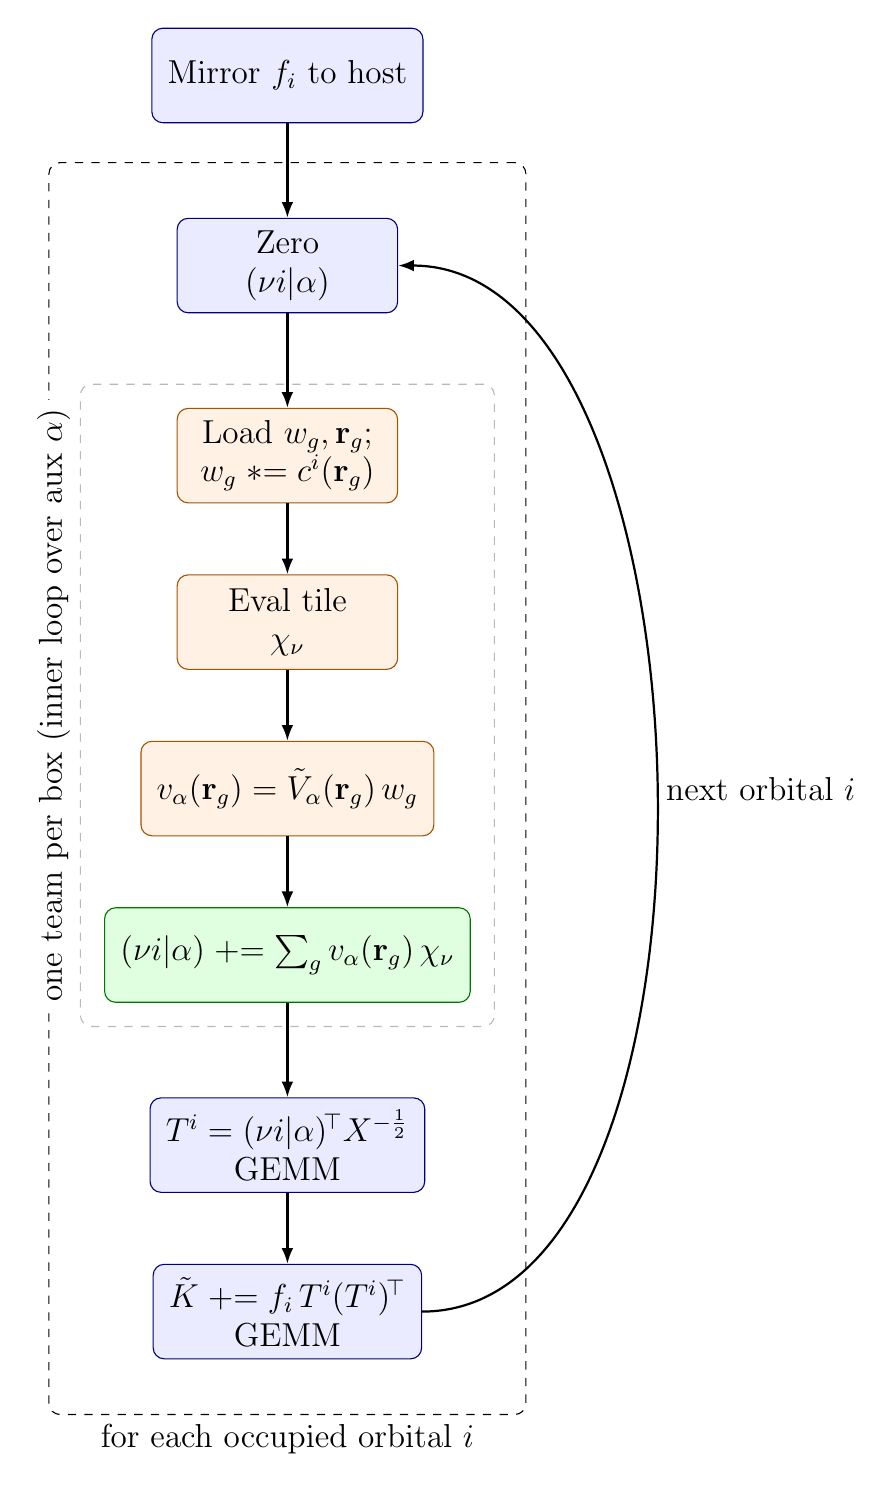
\begin{tikzpicture}[
        node distance=9mm,
        box/.style={draw, rounded corners, minimum height=12mm,
        minimum width=28mm, align=center, font=\large, inner xsep=2mm},
        hostbox/.style={box, fill=blue!8, draw=blue!50!black},
        databox/.style={box, fill=yellow!10, draw=yellow!65!black},
        threadbox/.style={box, fill=orange!10, draw=orange!65!black},
        teambox/.style={box, fill=green!12, draw=green!45!black},
        arr/.style={-{Latex[length=2mm]}, thick},
        looplabel/.style={font=\large, text=black!70!black}
      ]
      \node[hostbox] (mirror) {Mirror $f_i$ to host};
      \node[hostbox, below=12mm of mirror] (zero) {Zero\\$(\nu i|\alpha)$};
      \node[threadbox, below=12mm of zero] (fold)
      {Load $w_g,\mathbf r_g$;\\$w_g\mathrel{*}=c^i(\mathbf r_g)$};
      \node[threadbox, below=of fold] (phi) {Eval tile\\$\chi_\nu$};
      \node[threadbox, below=of phi] (pot)
      {$v_\alpha(\mathbf r_g)=\tilde V_\alpha(\mathbf r_g)\, w_g$};
      \node[teambox, below=of pot] (tci)
      {$(\nu i|\alpha)\mathrel{+}=\sum_g v_\alpha(\mathbf r_g)\,\chi_\nu$};
      \node[hostbox, below=12mm of tci] (gemm1)
      {$T^i=(\nu i|\alpha)^{\!\top}X^{-\frac12}$\\GEMM};
      \node[hostbox, below=of gemm1] (gemm2)
      {$\tilde K\mathrel{+}=f_i\,T^i(T^i)^{\!\top}$\\GEMM};
      \draw[arr] (mirror) -- (zero);
      \draw[arr] (zero) -- (fold);
      \draw[arr] (fold) -- (phi);
      \draw[arr] (phi) -- (pot);
      \draw[arr] (pot) -- (tci);
      \draw[arr] (tci) -- (gemm1);
      \draw[arr] (gemm1) -- (gemm2);
      \draw[arr] (gemm2.east) to[out=0, in=0, looseness=0.8]
      node[midway, right, looplabel] {next orbital $i$} (zero.east);
      \begin{scope}[on background layer]
        \node[draw, dashed, rounded corners, inner sep=7mm,
          fit=(zero)(fold)(phi)(pot)(tci)(gemm1)(gemm2),
        label={[looplabel]below:{for each occupied orbital $i$}}] {};
        \node[draw, dashed, draw=gray!55, rounded corners, inner sep=3mm,
          fit=(fold)(phi)(pot)(tci),
          label={[looplabel, fill=white, rotate=90, anchor=south]left:{one
        team per box (inner loop over aux $\alpha$)}}] {};
      \end{scope}
  \end{tikzpicture}}
  \caption{Control-flow of the neighbor-tiled RI-K kernel
    (\texttt{compute\_exact\_exchange\_tiled}). The occupied orbitals are
    treated one at a time: orbital $i$ is folded into the quadrature
    weights via $c^i(\mathbf r_g)=\sum_\lambda C^i_\lambda
    \chi_\lambda(\mathbf r_g)$, the
    three-center integral $(\nu i|\alpha)$ is built by the tiled team
    kernel (each neighbor tile of $\chi_\nu$ evaluated once and reused
    across all auxiliary functions $\alpha$), and $\tilde K_{\mu\nu}$ is
    accumulated by two host GEMMs applying $X^{-\frac12}$. Colors as in
  Figure~\ref{fig:tiled_rij_flow}.}
  \label{fig:tiled_rik_flow}
\end{figure}

\begin{table}[H]
  \centering
  {\small
    \begin{tabular}{@{}l l l l l@{}}
      \toprule
      Allocation & Type & Size & Symbol & Scope \\
      \midrule
      \texttt{three\_center\_integral} & \texttt{View<double**>}
      & $N_\text{aux}\times N_\text{bf}$ & $(\nu i|\alpha)$ & global \\
      \texttt{\ ..\_scaled}            & \texttt{View<double**>}
      & $N_\text{bf}\times K$            & $T^i_{\nu k}$ & global \\
      \texttt{result}                  & \texttt{View<double**>}
      & $N_\text{bf}\times N_\text{bf}$  & $\tilde K_{\mu\nu}$ & global \\
      \texttt{mo\_coeff\_h}            & host \texttt{View<double*>}
      & $N_\text{occ}$                   & $f_i$ & host \\
      \texttt{weights\_scratch}        & \texttt{View<double*, Scratch>}
      & $P_\text{max}$                   & $w_g\,c^i_g$ & per team \\
      \texttt{points\_scratch}         & \texttt{View<Point*, Scratch>}
      & $P_\text{max}$                   & $\mathbf r_g$ & per team \\
      \texttt{phi\_cache}              & \texttt{View<double*, Scratch>}
      & $\texttt{tile}\times P_\text{max}$ & $\chi_\nu$ tile & per team \\
      \texttt{potential\_scratch}      & \texttt{View<double*, Scratch>}
      & $P_\text{max}$                   & $v_\alpha(\mathbf
      r_g)$ & per team \\
      \bottomrule
  \end{tabular}}
  \caption{Memory allocations in
    \texttt{compute\_exact\_exchange\_tiled}. All device views use
    \texttt{Kokkos::LayoutLeft}; $P_\text{max}=\texttt{max\_points\_per\_box}$
    and $\texttt{tile}=\texttt{tile\_size}$ (default 32). The three
    global device matrices are reused across the loop over occupied
    orbitals; the per-team scratch footprint
    $(2+\texttt{tile})\,P_\text{max}$ doubles plus $P_\text{max}$ points
  is independent of the neighbor count.}
  \label{tab:tiled_rik_memory}
\end{table}

We should note that although this implementation takes advantage of
the locality that atomic orbitals provide, the repeated evaluation of
the basis functions becomes a massive computational cost. Another
thing to keep in mind when comparing the two implementations is that
due to the collocations being pre-computed in the dense linear
algebra version, we could in theory also offload the pre-computation
to another library, whereas in the locally dense version, we need to
be able to evaluate the basis functions within the kernel.

\section{Results}\label{sec:results}

This section contains the results obtained with our implementations.
We analyze convergence as well as timing results, starting with
preliminary studies on small example systems and then
later perform full benchmarks on the W4-11 set of Karton, Daon and
Martin~\cite{Karton11w411}.

\subsection{Convergence}\label{subsec:convergence}

We first need to understand how the choice of the underlying
quadrature grid affects our experiments. We therefore make an
incremental study of how the resolution and geometry of a chosen
quadrature grid affect the HF energies. We start with the hydrogen
atom, then move on to the dihydrogen cation and last
perform SCF computations on the water molecule. Where an exact value is
available in closed form we use it: the hydrogen atom is measured
against the analytic $1s$ energy $E_\mathrm{exact}=-0.5$~\( E_\mathrm
h \) and the
H$_2^+$ overlap against its analytic value. Everywhere else the energy
errors reported in this section are measured against a shared
self-reference, evaluated on a grid far finer than any grid in the
respective sweep, rather than against an exact or basis-set limit
value. Either way the comparison isolates the quadrature error from the
basis-set incompleteness error and lets us compare schemes on an equal
footing.

\subsubsection{The Hydrogen Atom}

The hydrogen atom only consists of one proton and one
electron. This allows us to study the convergence properties of the core
Hamiltonian in isolation. Since there is no two-electron contribution,
the accuracy reached here is a best case: it gives us a floor on the
error we can expect for larger systems, rather than a prediction of it.

We first test how well the radial grids presented in
Section~\ref{subsec:quadratures} compare against each other.
Figure~\ref{fig:conv_radial_h} shows that all three schemes converge
monotonically, with the (M4) grid being the most accurate at every
radial resolution and reaching \( 1.0 \times 10^{-15} \)~\( E_\mathrm
h \). The (M3)
grid is the slowest of the three and still sits at \( 6.4 \times
10^{-12} \)~\( E_\mathrm h \) on the finest grid of the sweep.
Because the reference
here is the analytic $1s$ energy rather than a self-reference, the (M4)
curve keeps descending across the whole sweep and only flattens once it
reaches the double-precision noise floor of the energy itself, at
roughly \( 10^{-15} \)~\( E_\mathrm h \). The full data is tabulated in
Table~\ref{tab:data_radial_h}. We used the QZ4P (ADF
Slater-type)\cite{VanLenthe2003} basis for this experiment.

Becke's proposed radial mapping is the least accurate of the three on
coarse grids, at \( n_\mathrm{rad}=10 \) it is more than two orders of
magnitude worse than (M3), but it overtakes (M3) from \(
n_\mathrm{rad}=40 \) onwards. From there on it sits between the (M3) and
(M4) grids. That it eventually beats (M3) is somewhat surprising, since
the (M3) grid was originally thought of as an improvement over Becke's
proposal.

\begin{figure}[htbp]
  \centering
  
\includegraphics[width=0.72\textwidth]{Visualisations/convergence_radial_h.pdf}
  \caption{We compute the lowest-MO energy of a single hydrogen atom
    for three radial quadrature
    schemes: Becke, Treutler--Ahlrichs (M3) ($\alpha=0$) and (M4)
    ($\alpha=0.6$), both with element scaling $\xi(\mathrm{H})=0.8$.
    As our basis set we chose QZ4P (ADF Slater-type).
    The angular grid is a Lebedev grid fixed
    at order $L=29$ (approx. 302 angular grid points). The radial point count
    is swept over
    $n_\mathrm{rad}\in\{10,20,40,80,160,320,640\}$. The reference is the
    exact non-relativistic $1s$ energy of the hydrogen atom,
    $E_\mathrm{exact}=-0.5$~\( E_\mathrm h \), so the ordinate
  $|E-E_\mathrm{exact}|$ is pure quadrature error.}
  \label{fig:conv_radial_h}
\end{figure}

\subsubsection{The Dihydrogen Cation H$_2^+$}

Before turning to energies, we verify the quadrature against a quantity
for which the exact answer is known in closed form. For two \( 1s \)
Slater functions with \( \zeta = 1 \), one centered on each proton at a
separation of \( R = 1 \)~bohr, the overlap integral is
\begin{equation}
  S_{AB} = e^{-R} \left( 1 + R + \frac{R^2}{3} \right)
  = \frac{7}{3} e^{-1} = 0.858385362733,
\end{equation}
so any deviation of the numerically integrated overlap is pure quadrature
error. Figure~\ref{fig:conv_h2plus} shows two one-dimensional sweeps of
this quantity. The radial sweep reaches an absolute error of \( 2.3
\times 10^{-14} \) at \( n_\mathrm{rad} = 200 \), while the angular sweep
is converged to the \( 10^{-14} \) level already at \( L = 23 \) and
merely fluctuates at that level afterwards. The atomic-centered quadrature
therefore reproduces a genuine two-center integral to essentially machine
precision, which tells us that the larger residual errors we observe below
are a property of the integrands and not of the implementation. The data
is tabulated in Table~\ref{tab:data_h2plus}.

\begin{figure}[htbp]
  \centering
  
\includegraphics[width=\textwidth]{Visualisations/convergence_h2plus.pdf}
  \caption{Convergence of the numerically integrated overlap integral
    $S_{AB}$ of H$_2^+$ towards its exact analytic value
    $S_\mathrm{exact}=\frac{7}{3}e^{-1}=0.858385362733$. The system is two
    $1s$ Slater functions with $\zeta=1$, one on each proton, at a
    separation of $R=1$~bohr. Radial scheme: Treutler--Ahlrichs; angular
    scheme: Lebedev. Left: radial sweep at a fixed angular order
    $L=59$(approx. 2400 angular grid points). Right: angular sweep at
    a fixed radial resolution
    $n_\mathrm{rad}=200$. Unlike the other convergence studies in this
    section, the reference here is exact rather than a self-reference. The
  full data set is listed in Table~\ref{tab:data_h2plus}.}
  \label{fig:conv_h2plus}
\end{figure}

To get a better understanding of the interplay between the radial
schemes and Becke's partitioning scheme, we analyze the convergence
behavior of the (M4) radial mapping and Becke's original radial
mapping. We compute the core Hamiltonian ground state energy of
H$_2^+$, i.e. \( 2 \)
protons and \( 1 \) electron, and perform a \( 2 \)-dimensional sweep
over radial and angular grid resolutions. The results of the \( 2
\)-dimensional sweeps are presented in Figure~\ref{fig:conv_2d} and
are tabulated in Tables~\ref{tab:data_2d_becke} and~\ref{tab:data_2d_m4}.

In Figure~\ref{fig:conv_2d} we can observe that the (M4) radial
mapping attains an error at least as low as Becke's for every grid
combination with \( n_\mathrm{rad} \geq 20 \), and a strictly lower one
wherever the radial rather than the angular quadrature is the limiting
factor. The one systematic exception is the coarsest radial grid, \(
n_\mathrm{rad}=10 \), where Becke's mapping is the better of the two at
every angular order---the same coarse-grid behavior we already observed
for the hydrogen atom. We should note though that for a fixed angular
order \( L \), once the error is dominated by the angular quadrature,
the error plateaus to the same value for both schemes when
increasing the radial grid resolution. Hence we can only expect the
(M4) radial mapping to yield superior results for a high enough
angular quadrature grid. The error is moreover not monotone in \( L \)
at fixed \( n_\mathrm{rad} \): at \( n_\mathrm{rad}=40 \) the (M4) error
grows from \( 7.4 \times 10^{-9} \)~\( E_\mathrm h \) at \( L=17 \)
to \( 1.7 \times
10^{-8} \)~\( E_\mathrm h \) at \( L=23 \), which we attribute to a partial
cancellation between the radial and angular quadrature errors that is
undone as the angular grid is refined. We decided to use the (M4) grid
for all further experiments, since we observed a faster convergence rate
and expect the (M4) grid to be the most cost-efficient choice.

\begin{figure}[htbp]
  \centering
  
\includegraphics[width=\textwidth]{Visualisations/convergence_2d.pdf}
  \caption{Two-dimensional (radial $\times$ angular) grid convergence of
    the H$_2^+$ core-Hamiltonian ground-state (lowest-MO) energy,
    comparing the Becke and Treutler--Ahlrichs (M4) radial schemes on a
    shared Lebedev angular grid. Molecule: H$_2^+$ with protons
    at $x=0$ and $x=1$~bohr; basis: QZ4P. Top left: radial convergence at
    the finest angular order in the sweep ($L=29$). Top right: angular
    convergence at the finest radial grid ($n_\mathrm{rad}=320$). Bottom:
    for each scheme, $|E-E_\mathrm{ref}|$ versus $n_\mathrm{rad}$ with one
    curve per angular order $L\in\{5,9,11,17,23,29\}$, illustrating that
    each radial curve plateaus at a floor set by the angular order (and
    vice versa). The reference is the mean of the two schemes on the
    finest grid ($n_\mathrm{rad}=640$, $L=41$),
    $E_\mathrm{ref}=-1.45175161440473$~\( E_\mathrm h \) (shared
      self-reference; the two
    schemes agree there to $7\times10^{-13}$~\( E_\mathrm h \)). The ordinate is
  $|E-E_\mathrm{ref}|$.}
  \label{fig:conv_2d}
\end{figure}

\subsubsection{Self-Consistent Field Calculations}\label{subsubsec:scf_calc}
Now that we have a clear grasp on how the quadrature grids affect the
convergence of simple systems, we are ready to perform the first full
SCF calculations. We analyze how the unrestricted Hartree--Fock
energy of water (H$_2$O) converges as the radial resolution and the
angular order are increased together. We ran the SCF cycles on an
unpruned grid, with Treutler angular grid pruning~\cite{Treutler1995}
and with Psi4's robust grid pruning~\cite{Smith2020}. The grid pruning
schemes are implemented in \texttt{IntegratorXX}~\cite{IntegratorXX}.

The pruning schemes are best explained by thinking of the quadrature
grid in terms of shells. A shell is defined as the collection of
quadrature points that have the same distance to the nucleus. In the
unpruned quadrature grid all shells have the same amount of points,
i.e. the angular order $L$ is the same for all shells. This approach is
wasteful, because regions close to the nucleus require fewer
quadrature points in order to be integrated accurately, as the
electron density is spherically symmetric inside the atom.
The Treutler pruning scheme fixes the order of the angular
shells closest to the nucleus to $L_\mathrm{inner} = 7$ and the
angular order in the
intermediate region to $L_\mathrm{intermediate} = 11$. The
Psi4's robust pruning scheme fixes
the order of the angular shells in the inner region to
$L_\mathrm{inner} = 7$ and the
angular order in the intermediate region to $L_\mathrm{intermediate}
= L-6$. The total HF-energies are presented in
Figure~\ref{fig:conv_pruning_total} and the energies of the individual
terms are presented in Figure~\ref{fig:conv_pruning_terms}. All
energies are tabulated in Table~\ref{tab:data_pruning}.

Note that the robust pruning scheme tracks the unpruned
scheme so closely that the two have the same error to three significant
figures at every grid level, while using roughly \( 30\% \) fewer
quadrature points
(\( 965\,422 \) instead of \( 1\,383\,454 \) points on the finest
grid). It therefore reduces the cost of the quadrature with no
discernible drawback. The Treutler pruning scheme, in contrast, appears
too aggressive in its pruning, as its total error plateaus above \(
10^{-5} \)~ \( E_\mathrm h \).

The per-term decomposition in Figure~\ref{fig:conv_pruning_terms}
explains both this accuracy floor and the non-monotonicity of the total
error. Both one-electron terms, \( E_\mathrm{kin} \) and \(
E_\mathrm{ne} \), converge one to two orders of magnitude more slowly
than the Coulomb and exchange terms and therefore limit the overall
accuracy, while the total error benefits from a partial cancellation
between the individual contributions and is consequently not monotone in
the grid size.

\begin{figure}[H]
  \centering
  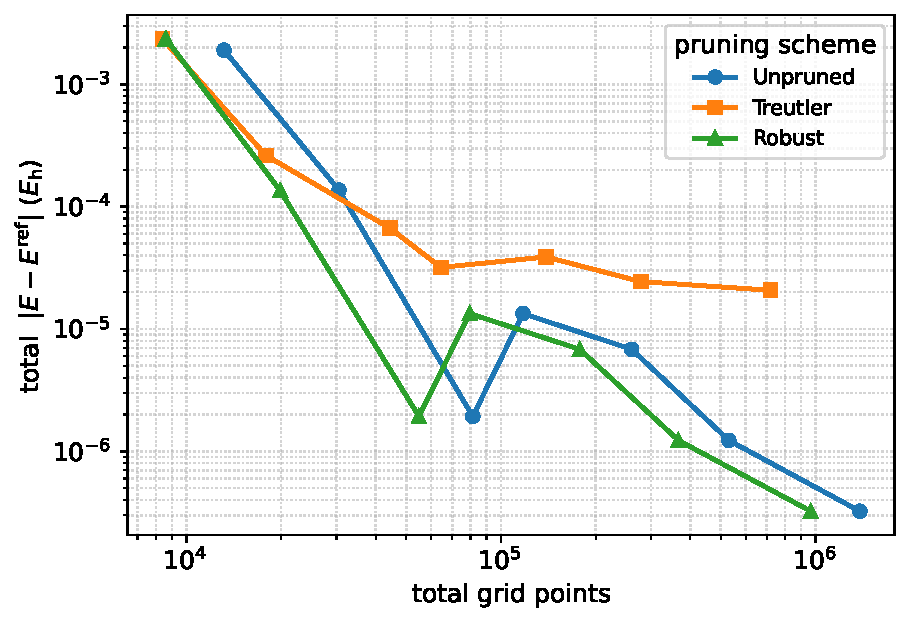
\includegraphics[width=0.72\textwidth]{Visualisations/convergence_pruning_total.pdf}
  \caption{Angular pruning-scheme comparison on water (H$_2$O):
    convergence of the \emph{total} unrestricted Hartree--Fock energy,
    plotted as accuracy per grid point. Schemes: \emph{Unpruned} (full
    Lebedev order on every radial shell), \emph{Treutler} (inner/middle
    shells fixed at Lebedev orders $7/11$) and \emph{Robust} (inner
      order $7$, middle order $\text{base}-6$, which tracks the base
    order). Radial scheme: TA-M4; angular: Lebedev; basis: QZ4P
    with QZ4P fit set; uniform radial sizing. Each grid level grows
    $n_\mathrm{rad}$ and the Lebedev order together, with
    $(n_\mathrm{rad},L)\in\{(40,17),(60,21),(90,28),(130,29),(200,35),
    (300,41),(600,45)\}$. The shared self-reference is a uniform
    unpruned grid with $n_\mathrm{rad}=1000$, $L=50$ ($2\,917\,774$
    points), $E_\mathrm{scf}=-76.0667767173$~ \( E_\mathrm h \). Note
    that the total
    error is not monotone: it results from the cancellation of the
    individual energy terms shown in
    Figure~\ref{fig:conv_pruning_terms}. The full data set is listed in
  Table~\ref{tab:data_pruning}.}
  \label{fig:conv_pruning_total}
\end{figure}

\begin{figure}[H]
  \centering
  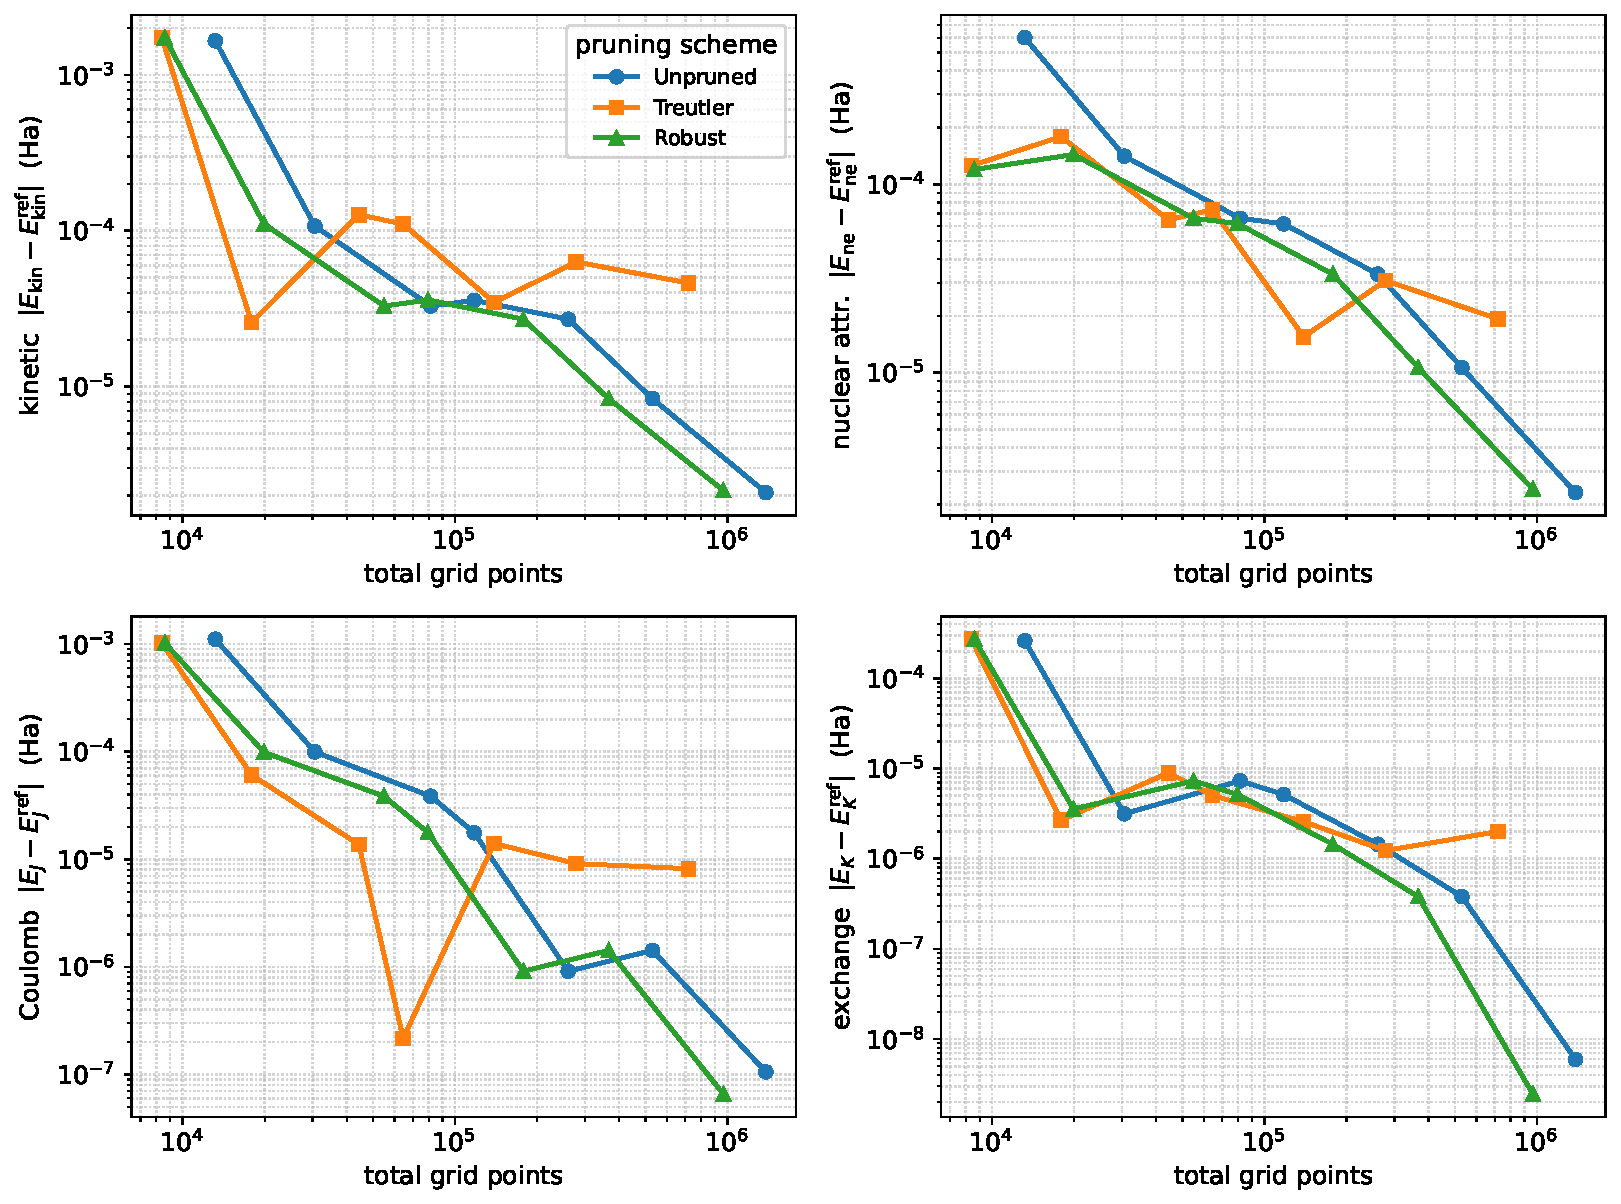
\includegraphics[width=\textwidth]{Visualisations/convergence_pruning_terms.pdf}
  \caption{Per-term decomposition of the angular pruning-scheme
    comparison of Figure~\ref{fig:conv_pruning_total}: absolute errors
    of the kinetic ($E_\mathrm{kin}$), nuclear-attraction
    ($E_\mathrm{ne}$), Coulomb ($E_J$) and exact-exchange ($E_K$)
    contributions to the unrestricted Hartree--Fock energy, against the
    total number of grid points. Systems, schemes, grids and reference
    as in Figure~\ref{fig:conv_pruning_total}; the reference values are
    $E_\mathrm{kin}=75.9976267410$~\( E_\mathrm h \),
    $E_\mathrm{ne}=-199.0472994426 $~\( E_\mathrm h \),
    $E_J=46.7402184304$~\( E_\mathrm h \) and $E_K=-8.9450726577$~\(
    E_\mathrm h \). The two
    one-electron terms converge one to two orders of magnitude more
    slowly than the two-electron terms and therefore limit the overall
    accuracy. The full data set is listed in
  Table~\ref{tab:data_pruning}.}
  \label{fig:conv_pruning_terms}
\end{figure}

\subsection{Benchmarks}\label{subsec:benchmarks}

In the previous section we established that our quadrature converges to
the level of a few $\mu$\( E_\mathrm h \). We now want to benchmark
the complete code
on a realistic workload. We ask two questions: how
well we can reproduce chemical quantities, and
where do our integration routines spend their time.

For both questions we use the W4-11 test set of Karton, Daon and
Martin~\cite{Karton11w411}, which collects $140$ total atomization
energies of small first- and second-row molecules. The reference values
are zero-point exclusive, non-relativistic and defined at clamped
nuclei. This is exactly the quantity that a difference of converged SCF
total energies gives, so no thermochemical or relativistic corrections
are needed. We run the whole set with the B3LYP hybrid
functional~\cite{Becke93b3lyp, Stephens1994} in each of the four ADF
Slater-type basis
sets DZ, TZP, TZ2P and QZ4P.\cite{VanLenthe2003} The set contains
$152$ distinct species,
which amounts to $608$ SCF calculations in total. All calculations use
the Treutler--Ahlrichs (M4) radial grid with $100$ radial points,
a Lebedev angular grid of order $L=35$ with the robust pruning scheme of
Section~\ref{subsubsec:scf_calc}, and the dense algorithm. We used
the superposition of atomic potentials (SAP)\cite{Lehtola2019c,
Lehtola2020} as the initial guess. The
SCF is run with \texttt{OpenOrbitalOptimizer}\cite{Lehtola2025} and
is converged to an orbital gradient of $10^{-6}$. All
timings were measured on a single GH200 GPGPU.

\iffalse
We had quite some trouble converging some of the open shell species.
Changing our initial guess from the core-Hamiltonian one to
the superposition of atomic potentials (SAP) \cite{Lehtola2020} helped but still
left us with a non-negligible amount of unconverged energies.
Therefore we exclude every
reaction that contains such a species rather
than report an unconverged energy, which leaves $139$,
$117$, $99$ and $103$ of the $140$ reactions for DZ, TZP, TZ2P and
QZ4P respectively; Table~\ref{tab:w411_species} lists the
convergence status of every species in the set.
\fi
Two caveats apply to the interpretation of the results. The quantity we
measure is the sum of the basis set incompleteness error and the
intrinsic error of the B3LYP functional. It is not a measure of the
numerical error of the integrator, which the previous section places
three to four orders of magnitude below the deviations reported here.
Furthermore, W4-11 deliberately contains several strongly
multireference species such as C$_2$ and FO$_2$, for which a single
determinant hybrid functional is not expected to work well.

\subsubsection{Energetic Accuracy}

Figure~\ref{fig:w411_violin} shows the distribution of the signed
atomization energy error for each basis set, and
Table~\ref{tab:w411_summary} collects the corresponding summary
statistics. The distributions narrow and shift towards zero
monotonically with growing basis size. The mean absolute deviation
improves from $51.8$~kcal/mol at DZ to $6.7$~kcal/mol at TZP,
$4.4$~kcal/mol at TZ2P and
$3.7$~kcal/mol at QZ4P. The DZ basis carries no polarization
functions at all
and underbinds so severely that it is of no quantitative use. Adding a
single polarization shell at TZP is by far the largest single
improvement, and the remaining progression to TZ2P and QZ4P is
comparatively modest. The QZ4P distribution settles at a mean signed
deviation of $-1.8$~kcal/mol rather than at zero. This residual is the
expected behavior of B3LYP itself and not a deficiency of our
integration, since the functional is known to underestimate atomization
energies.\cite{Bauschlicher1995} We take the agreement of this
progression with the published
behavior of B3LYP as evidence that the full pipeline of grid
construction, density fitting and exchange-correlation quadrature works
correctly on realistic chemistry.

\begin{figure}[H]
  \centering
  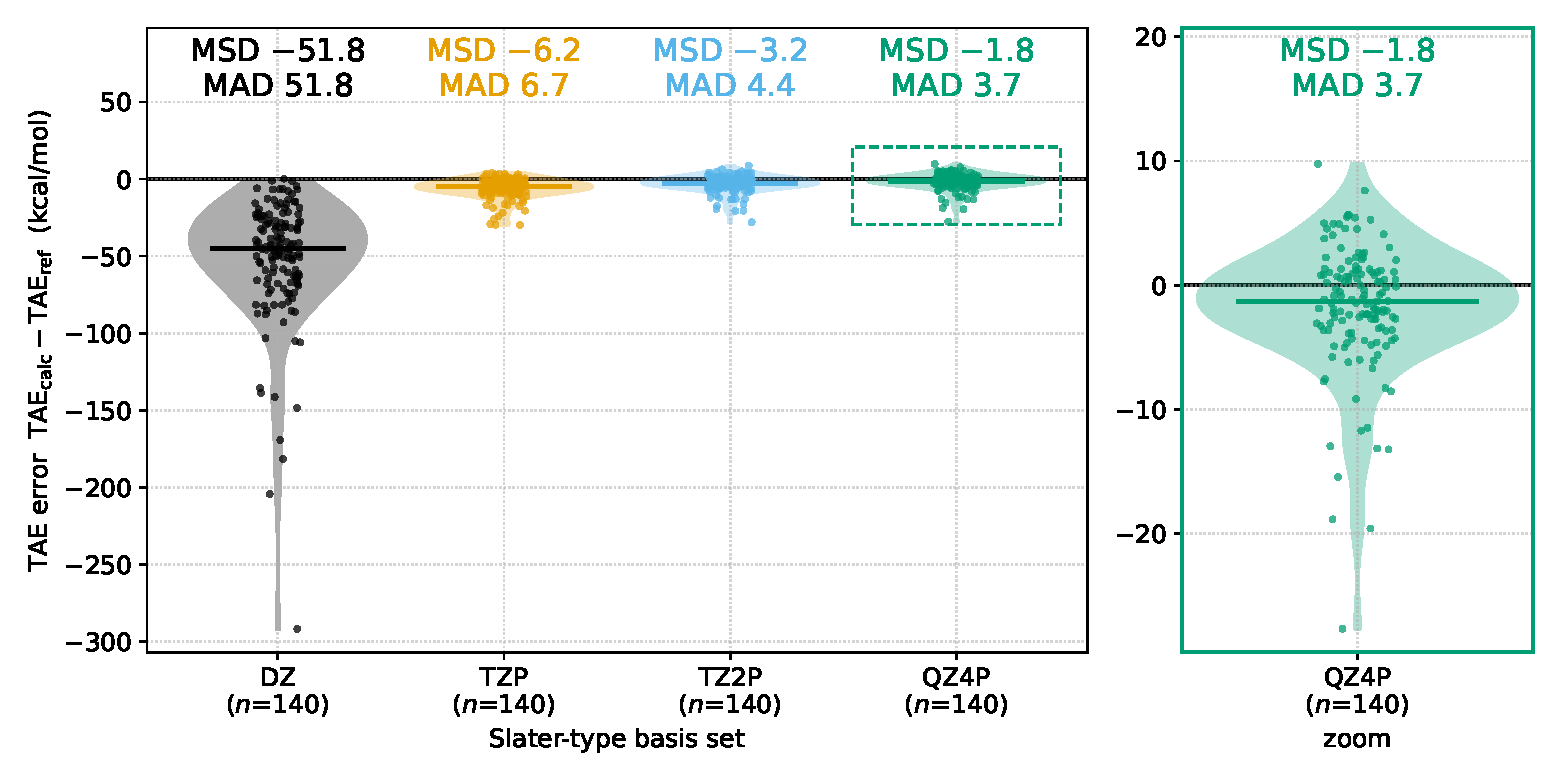
\includegraphics[width=0.78\textwidth]{Visualisations/benchmark_w411_violin.pdf}
  \caption{Distribution of the signed error in the W4-11 total
    atomization energies, one violin per Slater-type basis set, with the
    number of converged reactions given below each label. Method is
    unrestricted B3LYP (\texttt{Libxc}~\cite{Lehtola2018libxc}
    \texttt{hyb\_gga\_xc\_b3lyp}\cite{Stephens1994}) with the dense
    algorithm. The grid
    is TA-M4 radial
    with $n_\mathrm{rad}=100$ and Lebedev order $L=35$ with robust
    pruning and uniform radial sizing. The linear dependence threshold
    of $10^{-6}$ is applied uniformly to all four basis sets. Reference
    values are the zero-point exclusive, non-relativistic,
    clamped-nuclei atomization energies of Ref.~\citenum{Karton11w411}.
    Individual reactions are overlaid as jittered points and the
    horizontal bar marks the median. The summary statistics are given
  in Table~\ref{tab:w411_summary}.}
  \label{fig:w411_violin}
\end{figure}

\begin{table}[H]
  \centering
  \caption{Summary of the W4-11 B3LYP atomization energy errors per
    basis set. Listed are the number of reactions $N_\mathrm{rx}$ for
    which all species converged, the mean number of primary basis
    functions $\overline{N_\mathrm{bf}}$, the mean signed deviation
    (MSD), the mean absolute deviation (MAD), the root mean square
    deviation (RMSD), the largest absolute deviation and the mean wall
    time per species $\overline{t}$. The error statistics average over
    the $N_\mathrm{rx}$ reactions in which every species converged,
    whereas $\overline{N_\mathrm{bf}}$ and $\overline{t}$ average over
    the individual converged species; the two therefore run over
    different populations. Timings from runs that did not converge are
    excluded throughout, since a stalled SCF burns an unbounded number
    of Fock builds and would inflate the mean. Systems,
  method and grid as in Figure~\ref{fig:w411_violin}.}
  \label{tab:w411_summary}
  \small
\begin{tabular}{@{}lrrrrrrr@{}}
  \toprule
  Basis & $N_\mathrm{rx}$ & $\overline{N_\mathrm{bf}}$ & MSD & MAD & RMSD & max & $\overline{t}$ \\
   &  &  & (kcal/mol) & (kcal/mol) & (kcal/mol) & (kcal/mol) & (s) \\
  \midrule
  DZ & 139 & 29 & -52.88 & 52.88 & 66.85 & 293.68 & 1.5 \\
  TZP & 131 & 55 & -8.72 & 8.94 & 11.91 & 55.26 & 2.1 \\
  TZ2P & 118 & 79 & -5.64 & 6.23 & 9.06 & 51.65 & 3.3 \\
  QZ4P & 121 & 138 & -4.04 & 5.13 & 7.42 & 31.82 & 9.9 \\
  \bottomrule
\end{tabular}

\end{table}

\subsubsection{Cost and Time Distribution}

Figure~\ref{fig:w411_scaling} plots the measured wall time against the
number of primary basis functions. The left panel gives the total
runtime and the right panel the cost of a single Fock build. Dividing
by the number of Fock builds removes the variation in how many SCF
iterations each molecule happened to need, so the right panel isolates
the scaling of the integral kernels themselves.

We deliberately do not use the number of quadrature points on the
horizontal axis. With uniform radial sizing the molecular grid contains
$n_\mathrm{atoms}\times n_\mathrm{rad}\times n_\mathrm{ang}$ points
independent of the basis set, so it takes only as many distinct values
as there are molecule sizes in the set and cannot resolve the cost
differences between the four bases.

\begin{figure}[H]
  \centering
  
\includegraphics[width=\textwidth]{Visualisations/benchmark_w411_scaling.pdf}
  \caption{Wall time over the W4-11 set against the number of primary
    basis functions $N_\mathrm{bf}$, on log-log axes. The left panel
    shows the total program runtime including grid construction, basis
    loading and all SCF iterations. The right panel shows the mean wall
    time of one Fock build, that is the total time spent in Fock
    construction divided by the number of builds, which removes the per
    molecule variation in the SCF iteration count. Legend entries give
    the exponent $p$ of a least squares power law
    $t\propto N_\mathrm{bf}^{\,p}$ fitted to each basis set. The gray
    guides are $N^2$, $N^3$ and $N^4$ slopes anchored at the median of
    the data. Systems, method and grid are described in
  Figure~\ref{fig:w411_violin}.}
  \label{fig:w411_scaling}
\end{figure}

Figure~\ref{fig:w411_breakdown} decomposes the runtime into the
individual stages of the calculation, and the outcome is very clear.
In the small DZ basis the exchange-correlation quadrature dominates
with about three quarters of the accounted time. Its absolute cost however
stays nearly constant across the four basis sets, at roughly $0.55$ to
$0.62$~s per molecule, because it is bound by the size of the grid and
not by the size of the basis. The exact exchange build behaves in the
opposite way. It grows from $0.1$~s per molecule at DZ to $4.2$~s at
QZ4P, where it accounts for $82$ percent of the accounted runtime and
leaves grid construction, collocation, the core Hamiltonian, the
auxiliary overlap of the density fitting and the Coulomb build as minor
contributions. This is the expected consequence of evaluating $K$
through the density fitted route of Section~\ref{subsec:density_fitting}
once per spin channel in every iteration, and it identifies the exact
exchange kernel as the component where optimization would pay off most.

\begin{figure}[H]
  \centering
  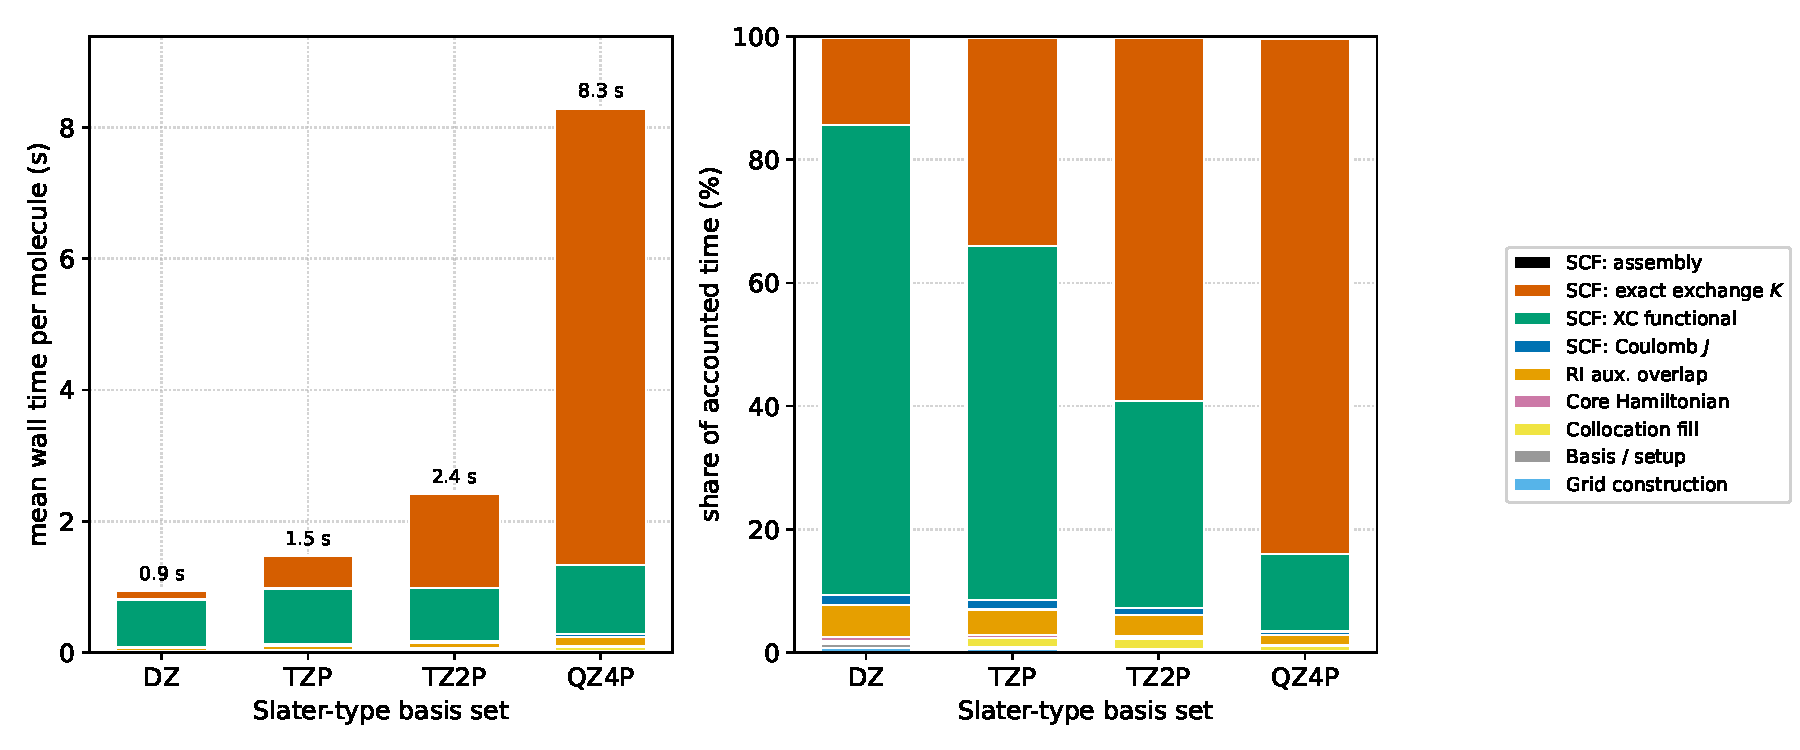
\includegraphics[width=\textwidth]{Visualisations/benchmark_w411_breakdown.pdf}
  \caption{Distribution of wall time over the stages of the
    calculation, averaged over all converged W4-11 species and summed
    over every SCF iteration of each run. The left panel shows the
    absolute mean wall time per species with the total annotated above
    each bar. The right panel shows the same data as a percentage of
    the accounted time, which makes the shift of work into the exact
    exchange build with growing basis size explicit. The first five
    categories are incurred once during start-up and the four labeled
    SCF once per Fock-matrix build. Systems, method and grid as in
  Figure~\ref{fig:w411_violin}. All timings use the dense algorithm.}
  \label{fig:w411_breakdown}
\end{figure}

\section{Conclusion} \label{sec:conclusion}

We found that the (M4) radial grid mapping has better convergence
properties than the (M3) and (Becke) radial mappings. In
Hartree--Fock calculations the error converges to within a few \(
\mu E_\mathrm h\), with the one-electron terms posing the accuracy
bottleneck; the two-electron terms converge to sub-\(\mu E_\mathrm h\)
levels for sufficiently dense quadrature grids.
Regarding pruning schemes we found that the Treutler pruning scheme
plateaus above \( 10^{-5} \)~Ha, whereas the Psi4's robust pruning
scheme reduces the number of quadrature points by about \( 30\%\) with
no discernible loss of accuracy.

Our benchmarks show that our quadratures in combination with
SCF libraries reproduce the published behavior of B3LYP on the
atomization energies of the W4-11 set. We observe a systematic
improvement towards the complete basis set limit going from DZ \( \to
\) TZP \( \to \) TZ2P \( \to \) QZ4P, which lowers the mean absolute
deviation from \( 51.8 \) to \( 3.7 \)~kcal/mol and leaves a residual
mean signed deviation of \( -1.8 \)~kcal/mol that reflects the
intrinsic underbinding of the functional rather than our integration.

The timings reveal that the cost shifts into the exact exchange build
as the basis grows: it is a minor contribution at DZ, where the
exchange-correlation quadrature dominates with about three quarters of
the measured runtime, but takes up \( 82\% \) of the computational time for
the QZ4P basis set. With an average build time rising from \( 0.07
\)~s per Fock matrix at DZ to \( 0.53 \)~s at QZ4P for molecules with
a handful of nuclei, the
usefulness of the library is still limited to very small systems. The
biggest benefit would come from optimizations in the locally dense
kernels from Section~\ref{subsubsec:locally_dense_la}, whose
implementations are still in a premature state.

Nevertheless, the reusability of the dense implementations should not
be understated. The integration kernels solely rely on a handful
of precomputed quantities, such as the collocation matrix, which can
be provided by the calling program. Our library opens access to
modern GPGPU computational power for Fock and Kohn--Sham
matrix assembly. The entire source code is publicly available on
\href{https://www.github.com/bobschreiner/NuKEXC}{https://www.github.com/bobschreiner/NuKEXC}
under the
\texttt{BSD 3-Clause License}.

\section{Further Research}\label{sec:further_research}

We believe that our library has the potential to accelerate the
exploration of NAOs. We initially planned to run the benchmarks with
NAOs constructed with HelFEM~\cite{Lehtola2019, Lehtola2019a}, but due
to time constraints we settled for STOs provided by
ADF~\cite{VanLenthe2003}, since they were readily
available and we could rely on more literature during the debugging
and testing of the code. We think that a study exploring the
convergence properties of the NAOs on polyatomic systems is of
great interest.

In future work we plan to extend the functionality of our library to
be able to handle meta-GGA functionals. At the time of writing, an
implementation of the
dense linear algebra algorithm to compute
$V_{\mu\nu}^\mathrm{meta-GGA}$ is present in the library for
spin-restricted systems,
but further testing is necessary to guarantee its correctness. The
overall structure of first building \( Z_\mu \) and
\(\bar{V}_{\mu\nu}^\mathrm{meta-GGA}\) and then symmetrizing is still
applicable, but requires the addition of terms relying on the kinetic
energy density.

At present the code can only handle small systems. Extending the
code with MPI would allow for distributed computing. Harnessing the
power of multiple GPUs will likely make it possible to study systems
substantially larger than the ones considered here. Since the most
computationally expensive part is a GEMM, and the Fock assembly can be
done with close to no communication overhead, we expect the parallel
scaling in the number of GPUs to be near linear.

To break past the barrier of moderately sized systems and move
towards extreme-scale calculations, the locally dense
implementations would need substantial optimizations. Our current
implementations require the basis functions to be evaluated on the
fly. At the time of writing, the kernels are latency-bound: they do not
expose enough independent work to hide memory and instruction latency,
and therefore cannot harness the full potential of GPGPUs, which
benefit from high arithmetic intensity and regular dense linear
algebra operations.

Another option to reduce the computational cost would be to reduce
the number of required quadrature points. We already observed that
robust pruning of the angular grids removes about \( 30\% \) of the
quadrature points at no cost in accuracy, which should translate into
a comparable saving in wall time, since the computational time grows
linearly with the grid size. Since the literature has been dominated
by GTOs, the published quadrature grids have also been optimized for
their integration. We expect that adaptive schemes that are
directly connected
to the convergence of the energies could yield improvements in
overall computational cost.

\section*{Acknowledgments}\label{sec:acknowledgments}

I want to thank Prof. Dr. Markus Reiher for enabling me to conduct my
thesis externally at the University of Helsinki. My thanks go to
Dr. Susi Lehtola for proposing the thesis project and for his
continued support and mentorship
throughout the writing of this thesis. I am grateful to Philip, Milan,
Hugo, Jonde, Kilian and Luukas for the moral support and positive
group mentality they provided in the office.
I also thank CSC -- IT Center for Science, Finland, for providing the
computational resources used for the experiments in this work.
Lastly, I want to thank my friends and partners for their support
outside of the working hours I spent on this thesis; without them I
would not have been able to finish this work.

\section*{AI transparency}\label{sec:AI transparency}

The following table contains a list of all tasks, that have been
facilitated by the use of generative artificial intelligence.
\begin{table}[H]
  \centering
  {\small
    \begin{tabular}{@{}l l l l@{}}
      \toprule
      Task & Model & Scope & Remarks   \\
      \midrule
      Grammar and spelling  &  Claude Opus 5 &  whole thesis & --- \\
      Content coherence   &  Claude Opus 5 &  whole thesis &
      Implemented relevant suggestions \\
      Plotting of figures & Claude  Opus 5 & all figures &
      Manually polished \\
      Tables & Claude  Opus 5 & all tables & Tables are generated
      from csv files  \\
      Derivation of unrestricted xc gga kernel
      & Claude  Opus 5 & section \ref{subsubsec:dense_la_xc}  &
      Formulas were rederived by hand \\
      Debugging of C++ code & Claude Opus 4.8\&5 & all codes & --- \\
      \bottomrule
  \end{tabular}}
  \caption{Table containing all the tasks that were supported by
  generative AI models}
  \label{tab:ai_transparency}
\end{table}

\appendix

\section{Convergence Data}\label{app:convergence_data}

\subsection{Hydrogen Atom: Radial Schemes}
\begin{table}[H]
  \centering\small
  \begin{tabular}{@{}rrlll@{}}
    \toprule
    $n_\mathrm{rad}$ & $N_\mathrm{quad}$ & $|E-E_\mathrm{exact}|$ Becke & $|E-E_\mathrm{exact}|$ TA-M3 & $|E-E_\mathrm{exact}|$ TA-M4 \\
    \midrule
    10 & 3,020 & $2.62\times10^{-2}$ & $1.62\times10^{-4}$ & $3.21\times10^{-6}$ \\
    20 & 6,040 & $1.11\times10^{-4}$ & $1.68\times10^{-5}$ & $5.18\times10^{-8}$ \\
    40 & 12,080 & $6.42\times10^{-8}$ & $1.05\times10^{-6}$ & $6.36\times10^{-10}$ \\
    80 & 24,160 & $1.03\times10^{-9}$ & $5.82\times10^{-8}$ & $6.57\times10^{-12}$ \\
    160 & 48,320 & $6.61\times10^{-11}$ & $2.97\times10^{-9}$ & $6.00\times10^{-14}$ \\
    320 & 96,640 & $4.18\times10^{-12}$ & $1.42\times10^{-10}$ & $2.00\times10^{-15}$ \\
    640 & 193,280 & $2.63\times10^{-13}$ & $6.39\times10^{-12}$ & $9.99\times10^{-16}$ \\
    \bottomrule
  \end{tabular}
  \caption{Radial-grid convergence data of the hydrogen-atom study (Figure~\ref{fig:conv_radial_h}). Absolute error of the core-Hamiltonian lowest-MO energy per radial scheme, measured against the exact non-relativistic $1s$ energy $E_\mathrm{exact}=-0.5$~$E_\mathrm{h}$.}
  \label{tab:data_radial_h}
\end{table}


\subsection{H$_2^+$: Overlap Integral}
\begin{table}[H]
  \centering\small
  \begin{tabular}{@{}lrrll@{}}
    \toprule
    sweep & param.\ & $N_\mathrm{quad}$ & $S_{AB}$ & $|S_{AB}-S_\mathrm{exact}|$ \\
    \midrule
    radial ($n_\mathrm{rad}$) & 10 & 23,990 & 0.859122134805 & $7.37\times10^{-4}$ \\
    radial ($n_\mathrm{rad}$) & 20 & 47,982 & 0.858383667212 & $1.70\times10^{-6}$ \\
    radial ($n_\mathrm{rad}$) & 30 & 71,964 & 0.858385391682 & $2.89\times10^{-8}$ \\
    radial ($n_\mathrm{rad}$) & 50 & 119,946 & 0.858385362390 & $3.43\times10^{-10}$ \\
    radial ($n_\mathrm{rad}$) & 75 & 179,918 & 0.858385362722 & $1.15\times10^{-11}$ \\
    radial ($n_\mathrm{rad}$) & 120 & 287,864 & 0.858385362733 & $3.79\times10^{-13}$ \\
    radial ($n_\mathrm{rad}$) & 200 & 479,774 & 0.858385362733 & $2.31\times10^{-14}$ \\
    \midrule
    angular ($L$) & 5 & 5,414 & 0.848794055322 & $9.59\times10^{-3}$ \\
    angular ($L$) & 10 & 19,814 & 0.858431911821 & $4.65\times10^{-5}$ \\
    angular ($L$) & 17 & 43,814 & 0.858385374009 & $1.13\times10^{-8}$ \\
    angular ($L$) & 23 & 77,414 & 0.858385362733 & $7.84\times10^{-14}$ \\
    angular ($L$) & 29 & 120,614 & 0.858385362733 & $3.97\times10^{-14}$ \\
    angular ($L$) & 35 & 173,246 & 0.858385362733 & $1.23\times10^{-14}$ \\
    angular ($L$) & 41 & 235,302 & 0.858385362733 & $1.80\times10^{-14}$ \\
    angular ($L$) & 53 & 388,758 & 0.858385362733 & $2.45\times10^{-14}$ \\
    \bottomrule
  \end{tabular}
  \caption{Convergence data of the H$_2^+$ overlap-integral study (Figure~\ref{fig:conv_h2plus}); $S_\mathrm{exact}=\frac{7}{3}e^{-1}=0.858385362733$.}
  \label{tab:data_h2plus}
\end{table}


\subsection{H$_2^+$: Radial $\times$ Angular Sweep}
\begin{table}[H]
  \centering\small
  \begin{tabular}{@{}rllllll@{}}
    \toprule
    $n_\mathrm{rad}$ \textbackslash\ $L$ & 5 & 9 & 11 & 17 & 23 & 29 \\
    \midrule
    10 & $6.59\times10^{-3}$ & $2.32\times10^{-3}$ & $3.62\times10^{-3}$ & $3.60\times10^{-3}$ & $3.60\times10^{-3}$ & $3.60\times10^{-3}$ \\
    20 & $1.20\times10^{-2}$ & $1.33\times10^{-3}$ & $7.38\times10^{-5}$ & $8.10\times10^{-5}$ & $8.02\times10^{-5}$ & $8.02\times10^{-5}$ \\
    40 & $1.21\times10^{-2}$ & $1.25\times10^{-3}$ & $2.78\times10^{-6}$ & $2.58\times10^{-7}$ & $2.88\times10^{-7}$ & $2.84\times10^{-7}$ \\
    80 & $1.21\times10^{-2}$ & $1.25\times10^{-3}$ & $2.55\times10^{-6}$ & $5.69\times10^{-9}$ & $2.53\times10^{-9}$ & $2.51\times10^{-9}$ \\
    160 & $1.21\times10^{-2}$ & $1.25\times10^{-3}$ & $2.55\times10^{-6}$ & $3.51\times10^{-9}$ & $1.85\times10^{-10}$ & $1.76\times10^{-10}$ \\
    320 & $1.21\times10^{-2}$ & $1.25\times10^{-3}$ & $2.55\times10^{-6}$ & $3.35\times10^{-9}$ & $2.01\times10^{-11}$ & $1.06\times10^{-11}$ \\
    \bottomrule
  \end{tabular}
  \caption{H$_2^+$ two-dimensional grid-convergence data, Becke radial scheme (Figure~\ref{fig:conv_2d}): $|E-E_\mathrm{ref}|$ in $E_\mathrm{h}$ for every combination of $n_\mathrm{rad}$ and angular order $L$.}
  \label{tab:data_2d_becke}
\end{table}

\begin{table}[H]
  \centering\small
  \begin{tabular}{@{}rllllll@{}}
    \toprule
    $n_\mathrm{rad}$ \textbackslash\ $L$ & 5 & 9 & 11 & 17 & 23 & 29 \\
    \midrule
    10 & $1.57\times10^{-2}$ & $5.79\times10^{-3}$ & $4.48\times10^{-3}$ & $4.47\times10^{-3}$ & $4.47\times10^{-3}$ & $4.47\times10^{-3}$ \\
    20 & $1.21\times10^{-2}$ & $1.27\times10^{-3}$ & $2.37\times10^{-5}$ & $2.46\times10^{-5}$ & $2.44\times10^{-5}$ & $2.43\times10^{-5}$ \\
    40 & $1.21\times10^{-2}$ & $1.25\times10^{-3}$ & $2.54\times10^{-6}$ & $7.44\times10^{-9}$ & $1.71\times10^{-8}$ & $1.78\times10^{-8}$ \\
    80 & $1.21\times10^{-2}$ & $1.25\times10^{-3}$ & $2.55\times10^{-6}$ & $2.85\times10^{-9}$ & $3.06\times10^{-10}$ & $2.52\times10^{-10}$ \\
    160 & $1.21\times10^{-2}$ & $1.25\times10^{-3}$ & $2.55\times10^{-6}$ & $3.33\times10^{-9}$ & $2.50\times10^{-12}$ & $6.80\times10^{-12}$ \\
    320 & $1.21\times10^{-2}$ & $1.25\times10^{-3}$ & $2.55\times10^{-6}$ & $3.33\times10^{-9}$ & $8.63\times10^{-12}$ & $9.07\times10^{-13}$ \\
    \bottomrule
  \end{tabular}
  \caption{H$_2^+$ two-dimensional grid-convergence data, M4 radial scheme (Figure~\ref{fig:conv_2d}): $|E-E_\mathrm{ref}|$ in $E_\mathrm{h}$ for every combination of $n_\mathrm{rad}$ and angular order $L$.}
  \label{tab:data_2d_m4}
\end{table}


\subsection{Water: Angular Pruning Schemes}
\begin{table}[H]
  \centering\small
  \begin{tabular}{@{}rrrlllll@{}}
    \toprule
    $n_\mathrm{rad}$ & $L$ & $N_\mathrm{quad}$ & $|\Delta E_\mathrm{kin}|$ & $|\Delta E_\mathrm{ne}|$ & $|\Delta E_J|$ & $|\Delta E_K|$ & $|\Delta E_\mathrm{tot}|$ \\
    \midrule
    \multicolumn{8}{@{}l}{\emph{Unpruned}} \\
    40 & 17 & 13,180 & $1.66\times10^{-3}$ & $6.00\times10^{-4}$ & $1.11\times10^{-3}$ & $2.61\times10^{-4}$ & $1.91\times10^{-3}$ \\
    60 & 21 & 30,568 & $1.07\times10^{-4}$ & $1.41\times10^{-4}$ & $9.94\times10^{-5}$ & $3.15\times10^{-6}$ & $1.36\times10^{-4}$ \\
    90 & 28 & 81,376 & $3.29\times10^{-5}$ & $6.60\times10^{-5}$ & $3.85\times10^{-5}$ & $7.30\times10^{-6}$ & $1.93\times10^{-6}$ \\
    130 & 29 & 117,542 & $3.58\times10^{-5}$ & $6.16\times10^{-5}$ & $1.76\times10^{-5}$ & $5.14\times10^{-6}$ & $1.34\times10^{-5}$ \\
    200 & 35 & 260,274 & $2.71\times10^{-5}$ & $3.33\times10^{-5}$ & $9.12\times10^{-7}$ & $1.45\times10^{-6}$ & $6.82\times10^{-6}$ \\
    300 & 41 & 530,152 & $8.37\times10^{-6}$ & $1.06\times10^{-5}$ & $1.42\times10^{-6}$ & $3.80\times10^{-7}$ & $1.23\times10^{-6}$ \\
    600 & 45 & 1,383,454 & $2.09\times10^{-6}$ & $2.31\times10^{-6}$ & $1.06\times10^{-7}$ & $5.96\times10^{-9}$ & $3.23\times10^{-7}$ \\
    \midrule
    \multicolumn{8}{@{}l}{\emph{Treutler}} \\
    40 & 17 & 8,392 & $1.74\times10^{-3}$ & $1.25\times10^{-4}$ & $1.02\times10^{-3}$ & $2.71\times10^{-4}$ & $2.36\times10^{-3}$ \\
    60 & 21 & 17,896 & $2.58\times10^{-5}$ & $1.79\times10^{-4}$ & $6.08\times10^{-5}$ & $2.67\times10^{-6}$ & $2.63\times10^{-4}$ \\
    90 & 28 & 44,368 & $1.27\times10^{-4}$ & $6.48\times10^{-5}$ & $1.37\times10^{-5}$ & $8.96\times10^{-6}$ & $6.67\times10^{-5}$ \\
    130 & 29 & 64,478 & $1.10\times10^{-4}$ & $7.33\times10^{-5}$ & $2.16\times10^{-7}$ & $5.02\times10^{-6}$ & $3.19\times10^{-5}$ \\
    200 & 35 & 139,098 & $3.47\times10^{-5}$ & $1.55\times10^{-5}$ & $1.40\times10^{-5}$ & $2.57\times10^{-6}$ & $3.88\times10^{-5}$ \\
    300 & 41 & 278,260 & $6.31\times10^{-5}$ & $3.08\times10^{-5}$ & $9.11\times10^{-6}$ & $1.23\times10^{-6}$ & $2.44\times10^{-5}$ \\
    600 & 45 & 718,822 & $4.62\times10^{-5}$ & $1.93\times10^{-5}$ & $8.17\times10^{-6}$ & $2.00\times10^{-6}$ & $2.07\times10^{-5}$ \\
    \midrule
    \multicolumn{8}{@{}l}{\emph{Robust}} \\
    40 & 17 & 8,608 & $1.73\times10^{-3}$ & $1.20\times10^{-4}$ & $1.02\times10^{-3}$ & $2.72\times10^{-4}$ & $2.36\times10^{-3}$ \\
    60 & 21 & 19,876 & $1.11\times10^{-4}$ & $1.44\times10^{-4}$ & $9.86\times10^{-5}$ & $3.56\times10^{-6}$ & $1.35\times10^{-4}$ \\
    90 & 28 & 54,880 & $3.29\times10^{-5}$ & $6.60\times10^{-5}$ & $3.85\times10^{-5}$ & $7.30\times10^{-6}$ & $1.93\times10^{-6}$ \\
    130 & 29 & 79,526 & $3.60\times10^{-5}$ & $6.19\times10^{-5}$ & $1.77\times10^{-5}$ & $5.15\times10^{-6}$ & $1.34\times10^{-5}$ \\
    200 & 35 & 178,050 & $2.71\times10^{-5}$ & $3.33\times10^{-5}$ & $9.12\times10^{-7}$ & $1.45\times10^{-6}$ & $6.82\times10^{-6}$ \\
    300 & 41 & 366,460 & $8.37\times10^{-6}$ & $1.06\times10^{-5}$ & $1.42\times10^{-6}$ & $3.80\times10^{-7}$ & $1.23\times10^{-6}$ \\
    600 & 45 & 965,422 & $2.16\times10^{-6}$ & $2.41\times10^{-6}$ & $6.57\times10^{-8}$ & $2.45\times10^{-9}$ & $3.23\times10^{-7}$ \\
    \bottomrule
  \end{tabular}
  \caption{Per-term convergence data of the water angular-pruning study (Figures~\ref{fig:conv_pruning_total} and~\ref{fig:conv_pruning_terms}): absolute errors of the kinetic, nuclear-attraction, Coulomb, exchange and total unrestricted Hartree--Fock energies. Reference: uniform unpruned grid with $n_\mathrm{rad}=1000$, $L=50$ (2,917,774 points), $E_\mathrm{kin}=75.9976267410$, $E_\mathrm{ne}=-199.0472994426$, $E_J=46.7402184304$, $E_K=-8.9450726577$, $E_\mathrm{scf}=-76.0667767173$~Ha.}
  \label{tab:data_pruning}
\end{table}


\section{Benchmark Data}\label{app:benchmark_data}

\subsection{W4-11: SCF Convergence Coverage}
{\small
\begin{longtable}{@{}lrrrrr@{}}
  \caption{Converged self-consistent field energies for every species of the W4-11 set, in each of the four Slater-type basis sets, with $2S+1$ the spin multiplicity. All species are neutral. Energies are given to $10^{-6}$~Ha; the archived CSV in \texttt{latex/Data/} carries the full ten decimals. A $\times$ marks a calculation that did not reach the convergence thresholds of Section~\ref{subsec:benchmarks}: such a run carries the solver's best-so-far rather than a variational energy, so no number is reported for it. Every reaction containing an unconverged species is excluded from the statistics of Table~\ref{tab:w411_summary}, which is how 24 species account for the reaction counts at the foot of this table.}
  \label{tab:w411_species}\\
    \toprule
    Species & $2S+1$ & \multicolumn{4}{c}{$E_\mathrm{SCF}$ (Ha)} \\
    \cmidrule(l){3-6}
     &  & DZ & TZP & TZ2P & QZ4P \\
    \midrule
    \endfirsthead
    \multicolumn{6}{@{}l}{\emph{\tablename~\thetable\ (continued)}}\\
    \toprule
    Species & $2S+1$ & \multicolumn{4}{c}{$E_\mathrm{SCF}$ (Ha)} \\
    \cmidrule(l){3-6}
     &  & DZ & TZP & TZ2P & QZ4P \\
    \midrule
    \endhead
    \midrule
    \multicolumn{6}{r@{}}{\emph{continued on next page}}\\
    \endfoot
    \midrule
    \multicolumn{2}{@{}l}{Reactions excluded} & 70 & 20 & 68 & 83 \\
    \multicolumn{2}{@{}l}{Reactions retained} & 70 & 120 & 72 & 57 \\
    \bottomrule
    \endlastfoot
    \texttt{acetaldehyde} & $1$ & $-153.702755$ & $-153.808215$ & $-153.815024$ & $-153.821452$ \\
    \texttt{acetic} & $1$ & $-228.892035$ & $-229.067433$ & $-229.077529$ & $-229.087284$ \\
    \texttt{al} & $2$ & $\times$ & $\times$ & $\times$ & $\times$ \\
    \texttt{alcl} & $1$ & $-702.577159$ & $-702.610729$ & $-702.612792$ & $-702.648958$ \\
    \texttt{alcl3} & $1$ & $-1622.966732$ & $-1623.083028$ & $-1623.091275$ & $-1623.164253$ \\
    \texttt{alf} & $1$ & $-342.244098$ & $-342.318892$ & $-342.321344$ & $-342.342510$ \\
    \texttt{alf3} & $1$ & $-541.961003$ & $-542.199390$ & $-542.207401$ & $-542.236023$ \\
    \texttt{alh} & $1$ & $-242.932358$ & $-242.943211$ & $-242.943480$ & $-242.960962$ \\
    \texttt{alh3} & $1$ & $-244.141080$ & $-244.163589$ & $-244.164442$ & $-244.181759$ \\
    \texttt{allene} & $1$ & $-116.566515$ & $-116.624651$ & $-116.631195$ & $-116.637120$ \\
    \texttt{b} & $2$ & $-24.643995$ & $\times$ & $-24.647339$ & $\times$ \\
    \texttt{b2} & $3$ & $\times$ & $-49.388209$ & $-49.388720$ & $\times$ \\
    \texttt{b2h6} & $1$ & $-53.220613$ & $-53.253851$ & $-53.257036$ & $-53.260112$ \\
    \texttt{be} & $1$ & $-14.658866$ & $-14.659336$ & $-14.659336$ & $-14.659372$ \\
    \texttt{be2} & $1$ & $-29.320037$ & $-29.324252$ & $-29.324704$ & $-29.324893$ \\
    \texttt{becl2} & $1$ & $-935.136962$ & $-935.206562$ & $-935.210001$ & $-935.248027$ \\
    \texttt{bef2} & $1$ & $-214.446594$ & $-214.626950$ & $-214.629948$ & $-214.636997$ \\
    \texttt{bf} & $1$ & $-124.589759$ & $-124.667413$ & $-124.671134$ & $-124.676448$ \\
    \texttt{bf3} & $1$ & $-324.377047$ & $-324.588621$ & $-324.598946$ & $-324.612263$ \\
    \texttt{bh} & $1$ & $-25.270498$ & $-25.278497$ & $-25.278953$ & $-25.280278$ \\
    \texttt{bh3} & $1$ & $-26.585573$ & $-26.596301$ & $-26.597641$ & $-26.598683$ \\
    \texttt{bhf2} & $1$ & $-225.124206$ & $-225.264404$ & $-225.271435$ & $-225.280592$ \\
    \texttt{bn} & $1$ & $-79.332605$ & $-79.370983$ & $-79.373302$ & $-79.375447$ \\
    \texttt{bn3pi} & $3$ & $-79.357814$ & $-79.401650$ & $-79.403440$ & $\times$ \\
    \texttt{c} & $3$ & $\times$ & $-37.839363$ & $-37.839378$ & $\times$ \\
    \texttt{c-hcoh} & $1$ & $-114.306755$ & $-114.401176$ & $-114.405893$ & $-114.411971$ \\
    \texttt{c-hono} & $1$ & $-205.512834$ & $-205.700688$ & $-205.709870$ & $-205.718399$ \\
    \texttt{c-hooo} & $2$ & $-225.886674$ & $-226.065073$ & $\times$ & $-226.084090$ \\
    \texttt{c-n2h2} & $1$ & $-110.517582$ & $-110.622330$ & $-110.626382$ & $-110.630795$ \\
    \texttt{c2} & $1$ & $-75.824565$ & $-75.864256$ & $-75.867069$ & $-75.869487$ \\
    \texttt{c2h2} & $1$ & $-77.272383$ & $-77.311073$ & $-77.316007$ & $-77.319914$ \\
    \texttt{c2h3f} & $1$ & $-177.710145$ & $-177.814451$ & $-177.821234$ & $-177.829009$ \\
    \texttt{c2h4} & $1$ & $-78.527445$ & $-78.564710$ & $-78.568797$ & $-78.572620$ \\
    \texttt{c2h5f} & $1$ & $-178.942510$ & $-179.047150$ & $-179.052802$ & $-179.060358$ \\
    \texttt{c2h6} & $1$ & $-79.757531$ & $-79.799323$ & $-79.802921$ & $-79.807027$ \\
    \texttt{cch} & $2$ & $-76.550759$ & $-76.589724$ & $-76.593682$ & $-76.597055$ \\
    \texttt{ccl2} & $1$ & $-958.197834$ & $-958.298206$ & $-958.305118$ & $-958.346261$ \\
    \texttt{cf} & $2$ & $-137.698126$ & $-137.784054$ & $\times$ & $-137.794527$ \\
    \texttt{cf2} & $1$ & $-237.546214$ & $-237.710923$ & $-237.719419$ & $-237.729573$ \\
    \texttt{cf4} & $1$ & $-437.196523$ & $-437.516817$ & $-437.533098$ & $-437.550917$ \\
    \texttt{ch} & $2$ & $-38.454632$ & $-38.472121$ & $-38.472947$ & $-38.475212$ \\
    \texttt{ch2-sing} & $1$ & $-39.095216$ & $-39.122168$ & $-39.123469$ & $-39.126022$ \\
    \texttt{ch2-trip} & $3$ & $-39.123234$ & $-39.141130$ & $-39.142628$ & $-39.144419$ \\
    \texttt{ch2c} & $1$ & $-77.203507$ & $-77.243620$ & $-77.246640$ & $-77.250421$ \\
    \texttt{ch2ch} & $2$ & $-77.843040$ & $-77.881370$ & $-77.885257$ & $\times$ \\
    \texttt{ch2f2} & $1$ & $-238.841723$ & $-238.996060$ & $-239.003446$ & $-239.012766$ \\
    \texttt{ch2nh} & $1$ & $-94.543767$ & $-94.613320$ & $-94.617285$ & $-94.621085$ \\
    \texttt{ch2nh2} & $2$ & $-95.119844$ & $-95.183933$ & $-95.188679$ & $\times$ \\
    \texttt{ch3} & $2$ & $-39.807670$ & $-39.826819$ & $-39.829024$ & $-39.830887$ \\
    \texttt{ch3f} & $1$ & $-139.656515$ & $-139.740905$ & $-139.745223$ & $-139.750805$ \\
    \texttt{ch3nh} & $2$ & $-95.105467$ & $\times$ & $-95.177235$ & $-95.181417$ \\
    \texttt{ch3nh2} & $1$ & $-95.767510$ & $-95.837614$ & $-95.841840$ & $-95.846281$ \\
    \texttt{ch4} & $1$ & $-40.481004$ & $-40.502289$ & $-40.504438$ & $-40.506484$ \\
    \texttt{cl} & $2$ & $-460.094252$ & $-460.097662$ & $-460.099113$ & $-460.117286$ \\
    \texttt{cl2} & $1$ & $-920.217701$ & $-920.278777$ & $-920.284938$ & $-920.322104$ \\
    \texttt{cl2o} & $1$ & $-995.300345$ & $-995.408253$ & $-995.417610$ & $-995.458168$ \\
    \texttt{clcn} & $1$ & $-552.849519$ & $-552.956912$ & $-552.965392$ & $-552.988074$ \\
    \texttt{clf} & $1$ & $-559.842591$ & $-559.925858$ & $-559.931990$ & $-559.955411$ \\
    \texttt{clo} & $2$ & $-535.170366$ & $-535.263451$ & $-535.270367$ & $\times$ \\
    \texttt{cloo} & $2$ & $-610.294429$ & $-610.426488$ & $-610.435295$ & $-610.460437$ \\
    \texttt{cn} & $2$ & $-92.636121$ & $-92.699558$ & $-92.703186$ & $-92.706087$ \\
    \texttt{co} & $1$ & $-113.217148$ & $-113.307075$ & $-113.312325$ & $-113.316613$ \\
    \texttt{co2} & $1$ & $-188.413628$ & $-188.580233$ & $-188.590851$ & $-188.597869$ \\
    \texttt{cs} & $1$ & $-436.092523$ & $-436.158661$ & $-436.161980$ & $-436.189126$ \\
    \texttt{cs2} & $1$ & $-834.291039$ & $-834.390242$ & $-834.398627$ & $-834.449890$ \\
    \texttt{dioxirane} & $1$ & $-189.454698$ & $-189.608509$ & $-189.616916$ & $-189.624008$ \\
    \texttt{ethanol} & $1$ & $-154.909186$ & $-155.014981$ & $-155.021551$ & $-155.028868$ \\
    \texttt{f} & $2$ & $-99.704784$ & $-99.737490$ & $-99.738498$ & $-99.742161$ \\
    \texttt{f2} & $1$ & $-199.432418$ & $-199.529724$ & $-199.533943$ & $-199.542450$ \\
    \texttt{f2co} & $1$ & $-312.787327$ & $-313.028892$ & $-313.042004$ & $-313.054478$ \\
    \texttt{f2o} & $1$ & $-274.521422$ & $-274.684196$ & $-274.691769$ & $-274.702941$ \\
    \texttt{fccf} & $1$ & $-275.561220$ & $-275.749389$ & $-275.761024$ & $-275.773326$ \\
    \texttt{fo2} & $2$ & $-249.907037$ & $-250.080115$ & $-250.089106$ & $-250.099302$ \\
    \texttt{foof} & $1$ & $-349.618404$ & $-349.844897$ & $-349.855245$ & $-349.868826$ \\
    \texttt{formic} & $1$ & $-189.600953$ & $-189.755774$ & $-189.764661$ & $-189.772456$ \\
    \texttt{glyoxal} & $1$ & $-227.632232$ & $-227.803323$ & $-227.813250$ & $-227.822166$ \\
    \texttt{h} & $2$ & $-0.498665$ & $-0.499038$ & $-0.499038$ & $-0.499056$ \\
    \texttt{h2} & $1$ & $-1.172094$ & $-1.172977$ & $-1.173493$ & $-1.173940$ \\
    \texttt{h2cn} & $2$ & $-93.905609$ & $-93.967051$ & $-93.970723$ & $\times$ \\
    \texttt{h2co} & $1$ & $-114.409817$ & $-114.493249$ & $-114.498702$ & $-114.503020$ \\
    \texttt{h2o} & $1$ & $-76.363663$ & $-76.428703$ & $-76.432442$ & $-76.436729$ \\
    \texttt{h2s} & $1$ & $-399.303797$ & $-399.345845$ & $-399.348440$ & $-399.372973$ \\
    \texttt{hccf} & $1$ & $-176.420728$ & $-176.534369$ & $-176.542837$ & $-176.550986$ \\
    \texttt{hcl} & $1$ & $-460.733976$ & $-460.761901$ & $-460.764459$ & $-460.783567$ \\
    \texttt{hcn} & $1$ & $-93.345216$ & $-93.411061$ & $-93.415411$ & $-93.418643$ \\
    \texttt{hcnh} & $2$ & $-93.885732$ & $\times$ & $-93.957911$ & $-93.962179$ \\
    \texttt{hcno} & $1$ & $-168.423712$ & $-168.561389$ & $-168.571568$ & $-168.577800$ \\
    \texttt{hco} & $2$ & $-113.758109$ & $-113.845508$ & $-113.850813$ & $\times$ \\
    \texttt{hcof} & $1$ & $-213.614769$ & $-213.772148$ & $-213.780879$ & $-213.789203$ \\
    \texttt{hf} & $1$ & $-100.392250$ & $-100.454441$ & $-100.457764$ & $-100.462790$ \\
    \texttt{hnc} & $1$ & $-93.329320$ & $-93.388576$ & $-93.393242$ & $-93.396487$ \\
    \texttt{hnco} & $1$ & $-168.526745$ & $-168.671800$ & $-168.680956$ & $-168.687267$ \\
    \texttt{hnnn} & $1$ & $-164.618039$ & $-164.771367$ & $-164.780318$ & $-164.785673$ \\
    \texttt{hno} & $1$ & $-130.354451$ & $-130.467202$ & $-130.472863$ & $-130.478853$ \\
    \texttt{hocl} & $1$ & $-535.827318$ & $-535.917057$ & $-535.923488$ & $-535.946168$ \\
    \texttt{hocn} & $1$ & $-168.485359$ & $-168.626859$ & $-168.635016$ & $-168.641895$ \\
    \texttt{hof} & $1$ & $-175.441337$ & $-175.549027$ & $-175.554184$ & $-175.561920$ \\
    \texttt{honc} & $1$ & $-168.399567$ & $-168.533535$ & $-168.541799$ & $-168.548695$ \\
    \texttt{hoo} & $2$ & $-150.796565$ & $-150.910248$ & $-150.916386$ & $-150.923290$ \\
    \texttt{hooh} & $1$ & $-151.436066$ & $-151.551079$ & $-151.557324$ & $-151.564592$ \\
    \texttt{hs} & $2$ & $-398.673647$ & $-398.698280$ & $-398.700427$ & $-398.724533$ \\
    \texttt{ketene} & $1$ & $-152.470669$ & $-152.582457$ & $-152.591079$ & $-152.597972$ \\
    \texttt{methanol} & $1$ & $-115.624679$ & $-115.710741$ & $-115.715862$ & $-115.721189$ \\
    \texttt{n} & $4$ & $-54.567570$ & $-54.580717$ & $-54.580720$ & $-54.581927$ \\
    \texttt{n2} & $1$ & $-109.419506$ & $-109.517536$ & $-109.522201$ & $-109.526965$ \\
    \texttt{n2h} & $2$ & $\times$ & $-110.022214$ & $-110.026686$ & $\times$ \\
    \texttt{n2h4} & $1$ & $-111.758971$ & $-111.855367$ & $-111.860215$ & $-111.864960$ \\
    \texttt{n2o} & $1$ & $-184.479777$ & $-184.653861$ & $-184.664723$ & $-184.671036$ \\
    \texttt{nccn} & $1$ & $-185.491359$ & $-185.626412$ & $-185.635212$ & $-185.642291$ \\
    \texttt{nh} & $3$ & $-55.187238$ & $-55.217377$ & $\times$ & $-55.220844$ \\
    \texttt{nh2} & $2$ & $-55.828757$ & $-55.874021$ & $-55.875894$ & $-55.878825$ \\
    \texttt{nh2cl} & $1$ & $-515.985134$ & $-516.065182$ & $-516.070276$ & $-516.091746$ \\
    \texttt{nh3} & $1$ & $-56.501757$ & $-56.552089$ & $-56.554715$ & $-56.557559$ \\
    \texttt{no} & $2$ & $-129.775425$ & $-129.885825$ & $-129.892293$ & $-129.898115$ \\
    \texttt{no2} & $2$ & $-204.884022$ & $-205.072525$ & $-205.083076$ & $\times$ \\
    \texttt{o} & $3$ & $-75.045824$ & $-75.068397$ & $\times$ & $-75.071292$ \\
    \texttt{o2} & $3$ & $-150.203986$ & $-150.323096$ & $-150.330371$ & $-150.338061$ \\
    \texttt{o3} & $1$ & $-225.222273$ & $-225.413538$ & $-225.424005$ & $-225.434288$ \\
    \texttt{oclo} & $2$ & $-610.118645$ & $-610.409549$ & $-610.426341$ & $-610.458401$ \\
    \texttt{ocs} & $1$ & $-511.351557$ & $-511.485689$ & $-511.495647$ & $-511.525277$ \\
    \texttt{of} & $2$ & $-174.788336$ & $-174.888457$ & $-174.893538$ & $-174.900760$ \\
    \texttt{oh} & $2$ & $-75.691222$ & $\times$ & $\times$ & $-75.742369$ \\
    \texttt{oxirane} & $1$ & $-153.644753$ & $-153.763350$ & $-153.770650$ & $-153.777359$ \\
    \texttt{oxirene} & $1$ & $-152.339670$ & $-152.452658$ & $-152.460649$ & $-152.468416$ \\
    \texttt{p} & $4$ & $-341.212659$ & $-341.213836$ & $-341.213836$ & $-341.235862$ \\
    \texttt{p2} & $1$ & $-682.545141$ & $-682.606007$ & $-682.608940$ & $-682.654547$ \\
    \texttt{p4} & $1$ & $-1365.073778$ & $-1365.276429$ & $-1365.289009$ & $-1365.384471$ \\
    \texttt{ph3} & $1$ & $-343.054132$ & $-343.097458$ & $-343.099392$ & $-343.122435$ \\
    \texttt{propane} & $1$ & $-119.036705$ & $-119.098342$ & $-119.103379$ & $-119.109456$ \\
    \texttt{propene} & $1$ & $-117.810314$ & $-117.869247$ & $-117.874788$ & $-117.880669$ \\
    \texttt{propyne} & $1$ & $-116.561257$ & $-116.622333$ & $-116.628645$ & $-116.634405$ \\
    \texttt{s} & $3$ & $-398.057309$ & $-398.060332$ & $\times$ & $-398.085131$ \\
    \texttt{s2} & $3$ & $-796.201074$ & $-796.278016$ & $-796.283898$ & $-796.333714$ \\
    \texttt{s2o} & $1$ & $-871.266062$ & $-871.491833$ & $-871.504001$ & $-871.559099$ \\
    \texttt{s3} & $1$ & $-1194.270986$ & $-1194.420298$ & $-1194.430895$ & $-1194.507364$ \\
    \texttt{s4-c2v} & $1$ & $-1592.379383$ & $-1592.571287$ & $-1592.584893$ & $-1592.686991$ \\
    \texttt{si} & $3$ & $-289.326778$ & $-289.329154$ & $-289.329163$ & $-289.349318$ \\
    \texttt{si2h6} & $1$ & $-582.429391$ & $-582.492404$ & $-582.495654$ & $-582.538048$ \\
    \texttt{sif} & $2$ & $-389.196520$ & $\times$ & $-389.291302$ & $\times$ \\
    \texttt{sif4} & $1$ & $-688.738531$ & $-689.149457$ & $-689.168101$ & $-689.204759$ \\
    \texttt{sih} & $2$ & $-289.930604$ & $\times$ & $-289.946908$ & $\times$ \\
    \texttt{sih3f} & $1$ & $-391.035954$ & $-391.160558$ & $-391.165768$ & $-391.190473$ \\
    \texttt{sih4} & $1$ & $-291.801743$ & $-291.838775$ & $-291.840475$ & $-291.861318$ \\
    \texttt{sio} & $1$ & $-364.598413$ & $-364.692111$ & $-364.695864$ & $-364.719301$ \\
    \texttt{so} & $3$ & $-473.207180$ & $-473.322284$ & $-473.329122$ & $-473.357402$ \\
    \texttt{so2} & $1$ & $-548.272655$ & $-548.580332$ & $-548.594182$ & $-548.627176$ \\
    \texttt{so3} & $1$ & $-623.279743$ & $-623.768852$ & $-623.791413$ & $-623.827708$ \\
    \texttt{ssh} & $2$ & $-796.788514$ & $-796.871874$ & $-796.878172$ & $\times$ \\
    \texttt{t-hcoh} & $1$ & $-114.317938$ & $-114.408216$ & $-114.413019$ & $-114.419546$ \\
    \texttt{t-hono} & $1$ & $-205.517171$ & $-205.700847$ & $-205.710481$ & $-205.719585$ \\
    \texttt{t-hooo} & $2$ & $-225.891417$ & $-226.064195$ & $\times$ & $-226.084281$ \\
    \texttt{t-n2h2} & $1$ & $-110.530325$ & $-110.629586$ & $-110.633611$ & $-110.639431$ \\
\end{longtable}
}


\bibliographystyle{unsrt}
\bibliography{Quadratures}


\includepdf{declaration-originality.pdf}

\end{document}
